\documentclass[fleqn]{wlscirep}
\usepackage[utf8]{inputenc}
\usepackage{lipsum}
\usepackage{amsmath}
\usepackage{amssymb}
\usepackage{amsfonts}
\usepackage{siunitx}
\usepackage{physics}
\usepackage{stmaryrd} % double brackets for jump operator
\usepackage{nameref}
\usepackage{booktabs}
\usepackage{makecell} % for table cells with line breaks
\usepackage{bm}
\usepackage{amsopn}
\usepackage[skip=10pt]{caption}
\usepackage{color}
\usepackage{xcolor,colortbl}
%\usepackage{soul}
\usepackage[nameinlink, capitalise]{cleveref}
\usepackage{graphicx}
\usepackage{graphbox} % for center-aligning figures vertically
\usepackage{tkz-euclide} % draw tikz pictures
\usepackage{subcaption}
\usepackage{tablefootnote} % for table footnotes
\usepackage{float} % figure placement

% Bibliography tools
\usepackage{csquotes}

% Set some cref options
\newcommand{\crefrangeconjunction}{--} % Change crefrange from "to" to dashed
\crefname{figure}{Figure}{Figure}

%% Some new commands
% Partial derivatives
\newcommand{\pdifft}[1]{\frac{\partial  #1}{\partial t}}
\newcommand{\pdiffx}[1]{\frac{\partial #1}{\partial x}}
\newcommand{\pdiffy}[1]{\frac{\partial #1}{\partial y}}
\newcommand{\pdiffxi}[1]{\frac{\partial #1}{\partial x_i}}
\newcommand{\pdiffxj}[1]{\frac{\partial #1}{\partial x_j}}
\newcommand{\secpdiffx}[1]{\frac{\partial^2 #1}{\partial x^2}}
\newcommand{\secpdiffxi}[1]{\frac{\partial^2 #1}{\partial x_i \partial x_i}}
\newcommand{\secpdiffxj}[1]{\frac{\partial^2 #1}{\partial x_j \partial x_j}}

% Norms
\newcommand{\normltwo}[1]{{ \vert\vert#1\vert\vert}_{L^2}}
\newcommand{\normltwovec}[1]{{ \vert\vert#1\vert\vert}_{\mathbf{L}^2}}
\newcommand{\normlinf}[1]{{\vert\vert#1\vert\vert}_{L^{\infty}}}
\newcommand{\Hnorm}[1]{\norm{#1}_{\mathbf{H}^1}}
\newcommand{\Hdivnorm}[1]{\norm{#1}_{\mathbf{H}(\mathrm{div};\Omega)}}

% Integrals
\newcommand{\dx}{\, \mathrm d\bm{x}}
\newcommand{\intO}[1]{\int_{\Omega}#1 \, \mathrm d\bm{x}}
\newcommand{\intG}[1]{\int_{\Gamma}#1 \, \mathrm ds}
\newcommand{\intF}[1]{\int_{\mathcal{F}_k}#1 \, \mathrm dS}
\newcommand{\intGnf}[1]{\int_{\Gamma_{\mathrm{nf}}}#1 \, \mathrm ds}
\newcommand{\intGinj}[1]{\int_{\Gamma_{\mathrm{inj}}}#1 \, \mathrm ds}
\newcommand{\intGin}[1]{\int_{\Gamma_{\mathrm{in}}}#1 \, \mathrm ds}
\newcommand{\intGout}[1]{\int_{\Gamma_{\mathrm{out}}}#1 \, \mathrm ds}
\newcommand{\intGinjout}[1]{\int_{\Gamma_{\mathrm{inj}}\cup\Gamma_{\mathrm{out}}}#1 \, \mathrm ds}
\newcommand{\intGs}[1]{\int_{\Gamma_s}#1 \, \mathrm ds}
\newcommand{\intGc}[1]{\int_{\Gamma_c}#1 \, \mathrm ds}
\newcommand{\intGp}[1]{\int_{\Gamma_p}#1 \, \mathrm ds}

% Domain and boundaries
\newcommand{\Gs}{\Gamma_{s}}
\newcommand{\Gc}{\Gamma_{c}}
\newcommand{\Gp}{\Gamma_{p}}
\newcommand{\Ginj}{\Gamma_{\mathrm{inj}}}
\newcommand{\Gnf}{\Gamma_{\mathrm{nf}}}
\newcommand{\Gin}{\Gamma_{\mathrm{in}}}
\newcommand{\Gout}{\Gamma_{\mathrm{out}}}

% Discontinuity operators
\newcommand{\avg}[1]{\{#1\}}
\newcommand{\jump}[1]{\llbracket#1\rrbracket}

% Bold faced math characters
\newcommand{\ff}{\mathbf{f}}
\newcommand{\nn}{\mathbf{n}}
\newcommand{\rr}{\mathbf{r}}
\newcommand{\uu}{\mathbf{u}}
\newcommand{\uuref}{\mathbf{u}_{\mathrm{ref}}}
\newcommand{\vv}{\mathbf{v}}
\newcommand{\ww}{\mathbf{w}}
\newcommand{\xx}{\bm{x}}
\newcommand{\JJ}{\mathbf{J}}
\newcommand{\VV}{\mathbf{V}}
\newcommand{\bsig}{\bm{\sigma}}
\newcommand{\bsigpar}{\hat{\bsig}_{\parallel}}
\newcommand{\bsigperp}{\hat{\bsig}_{\perp}}
\newcommand{\beps}{\bm{\varepsilon}}
\newcommand{\btau}{\bm{\tau}}

% Comments
\newcommand{\lyng}[1]{\textcolor{blue}{#1}}
\newcommand{\rt}[1]{\textcolor{red}{#1}}
\newcommand{\mer}[1]{\textcolor{magenta}{#1}}
\newcommand{\mk}[1]{\textcolor{olive}{MK: #1}}

\newcommand{\fixme}[1]{\textcolor{red}{#1}}

% Title
\title{The role of cilia-mediated cerebrospinal fluid flow in intraventricular transport in zebrafish embryos}
\author[1,*]{Halvor Herlyng}
\author[1]{Ada J.~Ellingsrud}
\author[1]{Miroslav Kuchta} 
\author[X]{Inyoung Jeong} % OK?
\author[1,3,+]{Marie E.~Rognes} % OK order?
\author[2,+]{Nathalie Jurisch-Yaksi}
\affil[1]{Department for Numerical Analysis and Scientific Computing, Simula Research Laboratory, Oslo, Norway}
\affil[2]{Department of Clinical and Molecular Medicine, Norwegian University of Science and Technology, Trondheim, Norway}
\affil[3]{K.~G.~Jebsen Center for Brain Fluid Research}
\affil[*]{\href{mailto:hherlyng@simula.no}{hherlyng@simula.no}}
\affil[+]{these authors contributed equally to this work}
% Optional PDF information
\ifpdf
\hypersetup{
  pdftitle={zebrafish-cilia-csf},
  pdfauthor={H.~Herlyng \textit{et al.}}
}
\fi

\begin{abstract}
    This paper presents ...
    %Flow of cerebrospinal fluid in zebrafish brain ventricles is studied in this work. Motivated by experimental observations, we consider motile cilia and cardiac beating as the driving flow mechanisms. A mathematical model of the flow is developed and coupled with a transport model to study the transport of molecules inside the brain ventricles. The Stokes equations are used to model the flow, with the motile cilia acting as a force on the fluid through a stress boundary condition that allows slip at the wall. Transport is modeled with an advection-diffusion equation coupled to the velocity field obtained from solving the Stokes equations. The flow and transport models are discretized with finite element methods. For the Stokes equations we employ a non-conforming discretization based on elements of the Brezzi-Douglas-Marini family. The advection-diffusion equation is discretized with discontinuous Galerkin elements. We implement and solve the discretized equations numerically to simulate flow and transport in a zebrafish brain ventricles geometry obtained with medical imaging.
\end{abstract}
\begin{document}
\maketitle
% Introduction:
% 1. What are cilia and why are they important?
% 2. Previous studies of cilia flow
% 3. What problem do we want to solve
% 4. The model and work done in this paper
\section*{Introduction}
\lyng{HH: This needs work, have just jotted down some stuff to have references ready.}

Development of brains and sustaining healthy functioning of the brain relies on a myriad of regulatory processes. One of these processes is the flow of cerebrospinal fluid (CSF) in the brain ventricles. The brain ventricles are hollow structures inside the skull where CSF is produced and flows around, transporting nutrients, neurotransmitters and other molecules important for neural development. 

The inner walls of the brain ventricles are lined with an epithelial cell layer. In some regions of the ventricles, motile cilia protrude the epithelial cell layer. Motile cilia are hair-like structures that beat in a metachronal wave pattern such as to generate a complicated flow pattern in the brain ventricles. Motile cilia are also found in other parts of the body where fluids are transport, such as the airways, liver and intestines. Regarding the function of motile cilia in the brain, it has previously been pointed out that further studies are needed for investigating their role~\cite{Eichele2020Cilia-drivenVentricle}, as well as the role of spatially organized CSF flow~\cite{Olstad2019CiliaryDevelopment}, in the development of the brain and its ventricular system.

Experiments~\cite{Olstad2019CiliaryDevelopment} have demonstrated that cilia induce a directional flow in the brain ventricles. In addition to the directional flow induced by motile cilia, a pulsatile component in the CSF flow in zebrafish ventricles has been observed~\cite{Olstad2019CiliaryDevelopment}. Cilia are also found to serve crucial roles in other organs than the brain. Motile cilia are essential for olfactory computations~\cite{Reiten2017Motile-Cilia-MediatedComputations}, and they are also fundamental to mucous transport in the trachea~\cite{Sleigh1988TheCilia}.

Early computational studies modeled ciliary transport of mucous in lungs with mathematics~\cite{Fulford1986Muco-ciliaryLung}. Propulsion of ciliated organisms has for some time been studied with mathematics~\cite{BLAKE1974MechanicsMotion}. According to Brennen~\emph{et al.}~\cite{Brennen1977FluidFlagella}, the study of cilia locomotion and fluid systems utilizing cilia sparked interest after a review on locomotion of protozoa microorganisms performed by Jahn~\emph{et al.}~\cite{Jahn1972LocomotionProtozoa}. Fine-scale interaction between single or several cilia and surrounding fluids has previously been analyzed with mathematics and numerics~\cite{Guo2020SimulatingGeometries, Ruvalcaba2021NumericalTree, Smith2009MathematicalFluids, Cui2019NumericalMethod, Cui2022AFlow}, also specifically for cilia in brain ventricles of zebrafish embryos~\cite{Salman2022ComputationalEmbryo}. Quantification of bulk flow and effects on bulk transport by cilia arrays (or sheets) have not been studied as much, though by some~\cite{Ramirez-SanJuan2020Multi-scaleArrays}. Two-dimensional modeling of flow and transport mediated by motile cilia in zebrafish brain central canal has previously been carried out~\cite{Thouvenin2020OriginCanal}. There is, however, very limited research on three-dimensional modeling of cilia-mediated flow and transport in brain ventricles. There are a couple of studies indicating that the effect of cilia on CSF flow is local in the human brain~\cite{Siyahhan2014FlowVentricles, Yoshida2022EffectVentricles}. Zebrafish ventricles are much smaller than human ventricles, meaning cilia play a larger role in establishing a CSF flow pattern. We wish to investigate the mechanisms of ciliary and cardiac-beating flow components, and how they each contribute to transport of molecules inside the brain ventricles.

In this paper, we present protein photoconversion experiments in zebrafish embryo brain ventricles, as well as a computational model of cerebrospinal fluid flow and protein transport.

\section*{Methods}
\label{sec:methods}

\mer{@HH: I suggest you write \cref{fig:figure1}\textbf{a}, rather than \cref{fig:figure1} panel \textbf{a}, throughout. Increases signal-to-noise ratio.}

\subsection*{Zebrafish maintenance and strains in photoconversion experiments}
The zebrafish~(\emph{danio rerio}) animal facilities used are approved by the Norwegian Food Safety Authority (NFSA, Mattilsynet). Furthermore, the zebrafish were maintained in accordance with the guidelines set by the NFSA and the European Communities Council Directive. The larval and adult zebrafish were raised under standard husbandry conditions at 28.5°C in a Techniplast Zebtech Multilinking system. The fish tanks were kept at constant pH 7.0 and 685 $\mu$S with a 14/10 hr light/dark cycle. From fertilization to 3 dpf, larvae were maintained in egg water (1.2 g marine salt and 0.1\% methylene blue in 20 L reverse osmosis (RO) water) and subsequently transferred to artificial fish water (AFW) (1.2 g marine salt in 20 L RO water). The zebrafish lines used in the experiments were \emph{ccdc103(dnaaf19)\textsuperscript{tn222a}} (\emph{schmalhans (smh)})~\cite{Jau-NianChen1997Left-rightZebrafish}(received from Drummond lab, MGH) and \emph{Tg(gfap:Gal4FF)\textsuperscript{nw7Tg}}~\cite{DiazVerdugo2019Glia-neuronSeizures}, \emph{Tg(5xuas:Signal-Dendra2)\textsuperscript{nw21Tg}}. Animals were in the pigmentless \emph{nacre\textsuperscript{b692}}(\emph{mitfa\textsuperscript{-/-}})~\cite{JamesA.Lister1999NacreFate} background.

Wholemount~\emph{in vivo} live imaging and photoconversion experiments were performed with zebrafish larvae at the 2 days post-fertilization (dpf) stage obtained from inbreeding of heterozygous \emph{smh\textsuperscript{+/-};Tg(gfap:Gal4FF);Tg(5xuas:Signal-Dendra2}) adult animals, as described by D’Gama~\emph{et al.}~\cite{DGama2024Cilia-mediatedBrain}. Controls consisted of either wild-type (\emph{smh}\textsuperscript{+/+}) or \emph{smh}\textsuperscript{+/-} heterozygous zebrafish from the same breeding. The mutants were identified based on their curved body~\cite{Jau-NianChen1997Left-rightZebrafish}.

\subsection*{Genotyping}
Genomic DNA (gDNA) was isolated from clipped fins of anesthetized adult fish using 100 $\mu$L of PCR lysis buffer (containing 1M tris pH 7--9, 0.5 M EDTA, tritonX-100, and Proteinase K 0.1 mg/ml) overnight at 50°C. To stop the lysis reaction, the samples were heated to 95°C for 10 minutes and then centrifuged at 13000 rpm for 2 minutes. The supernatant containing gDNA was utilized for KASP assays-based analysis. The gDNAs were diluted (1:2) with water, and 3 $\mu$L of the diluted gDNA was used to perform the KASP assay following the guidelines of the manufacturer (LGC Biosearch Technologies™). For each sample well, the master mix contained: 5 $\mu$L of master mix; 0.14 $\mu$L of assay mix; 1.86 $\mu$L of RO water.


\subsection*{Generation of \emph{Tg(5xuas:Signal-Dendra2)\textsuperscript{nw21Tg}} line}
\mer{MER: Could this heading be made understandable by non-experts?}
The open reading frame (ORF) of the neuropeptide y (npy) signal peptide (\emph{npy}: ENSDARG00000036222, Q1LW93) was fused with the N-terminal of zebrafish codon optimized Dendra2 DNA sequence. Next the conjugated DNA sequence was synthesized with EcoR1 enzyme sites at the 5’ and 3’ ends (GenScript Biotech), and the synthesized signal-Dendra2 DNA was inserted into the pT2MUASMCS vector~\cite{Asakawa2008GeneticZebrafish} through restriction enzyme cloning (GenScript Biotech).  To generate the transgenic line, the 5xuas:Signal-Dendra2 plasmid DNA was used. A volume of 2 nl of a mixture of the plasmid DNA (60 pg) and tol2 mRNA (10 pg) was microinjected into one-cell stage embryos, as described by Jeong~\emph{et al.}~\cite{Jeong2024TheZebrafish}. The injected embryos were raised to adulthood (F0). Germline-transmitted founder zebrafish were identified by breeding with multiple Gal4 transgenic lines. Stable F1 embryos expressing the Gal4-driven Dendra2 signals were screened and raised to adult zebrafish.

\subsection*{Wholemount zebrafish \emph{in vivo} live time-lapse imaging and photoconversion of Dendra2}
To image 2 dpf larval zebrafish, the fish were anesthetized in 0.013\% MS222 in AFW and mounted laterally in 1.5\% low melting agarose in a Flurodish (VWR, FD35PDL-100), to obtain a lateral view of the brain ventricles. After the fish were positioned in the agarose, the dish stood for 5 min to allow the agarose to solidify. After solidification, AFW containing 0.013\% MS222 was added, and then the fish were transferred to the confocal microscope (LSM880 Examiner, Zeiss) and imaged using a 20x water-immersion objective (Zeiss, NA 1.0, Plan-Apochromat) at room temperature.

The time-lapse images were acquired in a single plane, covering the telencephalic, diencephalic and rhombencephalic ventricles simultaneously, with a frequency of 0.37--0.38 Hz (2.60--2.68 sec / frame). The size of the images was $1024\times400$ pixels. In total, 300 images were acquired per fish. The first 10 images were scanned without photoconversion to obtain a baseline value of fluorescence intensity, and the next 290 images were scanned while performing photoconversion. For photoconversion, ‘Bleaching’ and ‘Region’ in the ZEN software were used. A 405 nm laser was focused into a circular area (diameter: 16 $\mu$m, scan 0.77 $\mu$sec/pixel) of the dorsoposterior diencephalic ventricle with 100\% laser power. The laser was illuminated in the area repeatedly between each scanning. After imaging, the fish health was checked and only data from healthy fish were analyzed.
Data were collected and analyzed from three separate experiments, with a total of 8 controls and 6 mutants.

\subsection*{Photoconversion data analysis}

Photoconversion data analysis was performed in MATLAB and the codes are \fixme{openly available\cite{zenodo-archive-for-repo-link-fixme}}. Following import of the image data, the photoconverted channel was aligned to correct for drift in $x,y$ directions using previously developed codes~\cite{Reiten2017Motile-Cilia-MediatedComputations, Ringers2023NovelEpithelia}. Only stable recordings were further analyzed. To increase the signal-to-noise ratio, the images were downsampled by a block average using a resampling factor of 6 (using the MATLAB function blockproc). The change of fluorescence $($$(F-F_0)/F_0$, hereafter referred to as $\Delta F$$)$ was calculated for each pixel at each time point of the data. Here, the value $F_0$ is the average fluorescence intensity for the baseline (the first 10 time-lapse images) acquired before photoconversion. 

To identify the time needed to pass a certain threshold value, $\Delta F$ values were first smoothened. The first timepoint when values surpassed the threshold was reported per pixel (in the downsampled images). A mask for the image was generated using the green (not photoconverted) channel and calculated on the block-averaged data based on the intensity being higher than 1.5x median intensity of all the frames.

In order to obtain $\Delta F$ values for a region of interest (ROI), ROIs were first drawn on the aligned and block-averaged time series. Six ROIs were drawn manually: ROI 1 at the location of photoconversion, and ROIs 2--6 in different regions of the ventricular system. The pixel values of the fluorescence intensity within one ROI are averaged for each time point, and the relative change $\Delta F$ is then calculated with this averaged value. To normalize the data with respect to photoconversion efficiency, the $\Delta F$ curves for all ROIs were divided by the $\Delta F$ values obtained for ROI 1 at the end of the experiment, so that $\Delta F$ values for the photoconverted site ROI 1 ranged from zero to one. Finally, we average the $\Delta F$ data from controls over the number of controls, and the data from mutants over the number of mutants. We report these mean values together with a one-standard deviation error band.


\subsection*{Intraventricular injection of microbeads and particle tracking}
In addition to photoconversion experiments, we carried out particle tracking inside the brain ventricles of a larval zebrafish, to demonstrate the motile-cilia and cardiac-cycle related flow features observed and described in Olstad~\emph{et al.}~\cite{Olstad2019CiliaryDevelopment}. A schematical illustration of the flow features in the brain ventricles is shown in~\cref{fig:figure1}, panel \textbf{a}. Our experimental setup for the particle tracking is identical to the ones considered there (\lyng{HH: Is this true?}), and we refer to that paper for further details than the ones provided here in the following.

Anesthetized 2 dpf control zebrafish were injected with 1 nl of a mixture containing 0.1\% w/v fluorescent beads (SPHERO Fluorescent Yellow Particles 1\% w/v, $F = 0.16$ mm) diluted in 7.5 mg/ml 70 kDa rhodamine B isothiocyanate-dextran (RITC-dextran; Sigma-Aldrich, R9379) dissolved in artificial CSF. Artificial CSF composition was as follows: 124 mM NaCl, 22 mM D-(+)-Glucose, 2.0 mM KCl, 1.6 mM MgSO\textsubscript{4} $\cdot$ 7 H\textsubscript{2}O, 1.3 mM KH\textsubscript{2}PO\textsubscript{4}, 24 mM NaHCO\textsubscript{3}, 2.0 mM CaCl\textsubscript{2} $\cdot$ 2 H\textsubscript{2}O. The needles used for the injections were pulled with a Sutter Instrument Co. Model P-2000 from thin-walled glass capillaries (1.00 mm; VWR) and cut open with a forceps. A volume of 1 nl of the solution was injected with a pressure injector (Eppendorf Femtojet 4i) in the rostral rhombencephalic ventricle. The pressure and time were calibrated for each needle using a 0.01 mm calibration slide.

Following injection, the zebrafish was directly placed under the confocal microscope and 1200 images were acquired at a frequency of 13.1 Hz. A single optical section was obtained. Particle tracking was done using TrackMate~\cite{Tinevez2017TrackMate:Tracking} in Fiji/ImageJ~\cite{Schindelin2012Fiji:Analysis} and plotted using MATLAB, as described by Jeong~\emph{et al.}~\cite{Jeong2022MeasurementTelencephalon}. The parameters for TrackMate were as follows. The DoG detector was used with the settings: threshold: 2.0, with median filtering; radius: 2.0, with subpixel localization. Next, the Simple LAP tracker was used with settings: max frame gap: 2; alternative linking cost factor: 1.05; linking max distance: 5.0; gap closing max distance: 2.0; splitting max distance: 15.0; allow gap closing: true; allow track splitting: false; allow track merging: false; merging max distance: 15.0; cutoff percentile: 0.9. Only the particle tracks with at least 30 data points, while simultaneously covering a distance of at least 8.8 $\mu$m, were shown (\cref{fig:figure1}, panels \textbf{b} and \textbf{c}).

\subsection*{Image-based computational geometries of zebrafish brain ventricles}
We generated a 3D representation of the brain ventricular walls using confocal imaging data of a zebrafish embryo injected intraventricularly with a 70 kDa dye at 2 dpf~\cite{Olstad2019CiliaryDevelopment}. From the imaging data, we constructed a computational mesh of the ventricles (\cref{fig:figure1}, panel \textbf{d}). The interior volume was meshed with fTetWild~\cite{Hu2020FastWild}. The \emph{standard} mesh consisted of 132 134 tetrahedral cells and had a maximal (minimal) \mer{edge length} of 14.9 $\mu$m (4.68 $\mu$m). At 2 dpf, the ventricular system consists mainly of 3 cavities: the telencephalic  (anterior), the di-/mesencephalic  (middle) and the rhombencephalic (posterior) ventricles, which are connected by ducts. Parts of the ventricular surfaces were marked to be lined with motile cilia~\cite{Olstad2019CiliaryDevelopment} (\cref{fig:figure1}\textbf{d}, pink markers).
\mer{MER: @HH: Check if you mean edge length or mesh cell size here.}
\begin{figure}%[hbt!]
    \centering
    \includegraphics[width=\linewidth]{graphics/figure1.png}
    \caption{\lyng{Experimenting with velocity colorbars, thoughts on the two options? Or have two separate as it is now?}}
    \label{fig:figure1}
\end{figure}

%\subsection*{Computational geometry variations}
The morphology and geometry of the brain ventricles vary across zebrafish individuals, and under physiological and pathological conditions. Motivated by an interest in how geometry impacts solute distribution, we also consider four variations in the ventricular geometry: by shrinking the fore-mid brain connection, the middle ventricle, the mid-hind brain connection, and all three simultaneously. We used Blender~\cite{Community2018BlenderPackage} to modify the brain ventricles geometry. \mer{MER: More specifics (i.e.~1 sentence and/or inserted info) here on how much these were shrunk and how.}

%% The brain ventricular geometry varies significantly across zebrafish individuals, both healthy and sick animals. Motivated by an interest in how these variations can impact solute transport in the brain ventricles, we study the impact on simulation results when modifying the computational geometry and mesh in four different scenarios. Because our computational mesh is inflated by the dye-injection performed before image segmentation, we study four different mesh versions where we shrink: the fore-mid brain connection; the middle ventricle; the mid-hind brain connection; and all of the three above simultaenously. We used Blender~\cite{Community2018BlenderPackage} to modify the brain ventricles geometry.



\subsection*{Computational CSF dynamics}

The beating motion of the cilia generates CSF flow with steady rotational structures~\cite{Olstad2019CiliaryDevelopment} within the brain ventricles (\cref{fig:figure1}, panels \textbf{a}--\textbf{c}). In addition, cardiac pulsations induces pulsatile CSF flow. We model this flow of CSF in the brain ventricles by the time-dependent, incompressible Stokes equations which read as follows. Find the CSF velocity $\uu = \uu(\xx, t) = (u_x(\xx, t), u_y(\xx, t), u_z(\xx, t))$ and the CSF pressure $p = p(\xx, t)$ for $\xx \in \Omega$ and time $t>0$, such that
\begin{subequations}
    \begin{align}
      \rho \pdifft{\uu} - \nabla \cdot \bsig &= \mathbf{0}
      \quad \text{in } \Omega,
      \label{eq:stokes_eq_mom}\\
      \nabla \cdot \uu &= 0
      \quad  \text{in } \Omega,
  \end{align}
  \label{eq:stokes_eqs}% 
\end{subequations}%
where the stress tensor is defined as $\bsig(\uu, p) = 2\mu\beps(\uu) - p\mathbf{I}$ and $\beps(\uu) = \frac{1}{2}\left(\nabla \uu + (\nabla\uu)^T\right)$ is the strain-rate tensor. Bold-face characters denote vectors or tensors, and $\mathbf{I}$ is the identity tensor in three dimensions. Furthermore, $\rho$ is the CSF density and $\mu$ is the dynamic viscosity of the CSF. We introduce the tangential traction $\bsigpar$ as the tangential component of the traction $\hat{\bsig}=\bsig\nn$:
\begin{equation*}
    \bsigpar = P_{\nn}(\hat{\bsig}) = (\mathbf{I} - \nn\otimes\nn)\hat{\bsig},
\end{equation*}
where $\nn$ is the outer unit normal of the boundary surface $\Gamma = \partial\Omega$, and $P_{\nn}(\rr)$ is the tangential  projection of a vector $\rr$ onto $\Gamma$. We consider three types of boundary conditions:  (i) \emph{tangential traction} (no flow normal to the boundary $\uu \cdot \nn = 0$ with a force $\btau$ applied tangentially on the boundary $\bsigpar = \btau$), (ii) \emph{normal pressure} (a pressure $\Tilde{p}$ applied in the normal direction: $(\mu\nabla\uu - p\mathbf{I})\nn = \Tilde{p}(t)\nn$), and (iii) \emph{free slip} (no flow normal to the boundary $\uu \cdot \nn = 0$ and no tangential forces $\bsigpar = {\bf 0}$). Unless noted otherwise, the free-slip condition is applied on the boundary. We use the initial condition\mer{s} $\uu(\xx, 0)=\mathbf{0}$ \mer{and $p(\xx, t) = 0$} for all $\xx\in\Omega$. \mer{MER: I don't think you use an initial condition on the pressure. Please check and remove if so. You can also just write: ``We assume that the system starts at rest ($\uu(t = 0) = \mathbf{0}$)''.}

\subsection*{Cilia-driven flow}
On the ciliated regions of the ventricle walls $\Gc$ (\cref{fig:figure1}, panel \textbf{d}), we impose a constant-in-time tangential traction $\bsigpar=\btau$ to represent the net forces of the cilia acting on the CSF. We set $\btau(\xx, \rr) = \tau \lambda(\xx) P_{\nn}(\rr)$, where the function $\lambda(\xx)$ and the sign of the vector $\rr=\pm(1, 0, 1)$ varies depending on the cilia region (see~\cref{subsec:appendixA1}). Both $\rr$ and the value $\tau=6.5\times 10^{-4}$ Pa were chosen by model calibration against the experimental data~\cite{Olstad2019CiliaryDevelopment}.

\subsection*{Flow induced by cardiac pulsations}\label{subsec:pressure_bcs}
To drive a cardiac-induced pulsatile flow inside the brain ventricles, we set $\Tilde{p}(t)=0$ and $\Tilde{p}(t)=-A\sin{\omega t}$ on anterior and posterior parts of the boundary $\Gp$~(\cref{fig:figure1}, panel \textbf{d}, blue markers). The amplitude $A=1.5\times 10^{-3}$ Pa determines the magnitude of the pulsatile flow, and was calibrated based on experimental data~\cite{Olstad2019CiliaryDevelopment}. The angular cardiac frequency $\omega=2\pi f=6.97$ rad/s was set based on a measured cardiac frequency of $f=2.22$ Hz.

%% \iffalse
%% \subsection*{Computational cerebrospinal fluid dynamics in a moving reference frame}
%%  An Arbitrary Lagrangian Eulerian (ALE) formulation~\cite{san2009convergence} is used as an alternative to the normal pressure boundary conditions to model back-and-forth flow induced by cardiac pulsations. In a reference frame moving with a velocity $\uuref=(A_{\mathrm{ref}}\sin{\omega t}, 0, 0)$, we reformulate the Stokes equations~\eqref{eq:stokes_eqs} using an ALE formulation:
%% \begin{subequations}
%%     \begin{alignat}{2}
%%         \rho\bigg(\pdifft{\uu} + (\uu_{\mathrm{ref}}\cdot\nabla)\uu\bigg) &= \nabla\cdot\bm{\sigma}(\uu, p), \label{eq:mom_eq_ALE}\\
%%         \nabla\cdot\uu &= 0.
%%     \end{alignat}
%%     \label{eq:stokes_eqs_ALE}%
%% \end{subequations}%
%% We then solve for the velocity $\mathbf{w} = \uu - \uuref$ in the moving reference frame, where $\uu$ is the velocity in the fixed reference frame. The amplitude $A_{\mathrm{ref}}=919$ $\mu$m/s, calibrated based on experimental data, determines the magnitude of the pulsatile flow, and $\omega=2\pi f$ is the angular cardiac frequency. In the ALE formulation, we consider the impermeability boundary condition $\mathbf{w}\cdot\nn=0$ in the normal direction and the free-slip boundary condition $\bsigpar(\mathbf{w}, p) = \mathbf{0}$ in the tangential direction.
%% \fi

\subsection*{Computational model of solute transport after photoconversion}
We simulate transport of photoconverted proteins within the brain ventricles by modeling transport of a solute with concentration $c(\xx, t)$ for $\xx\in\Omega$ and time $t > 0$ by the advection-diffusion equation
\begin{equation}
    \pdifft{c} + \nabla\cdot\JJ = 0 \quad \text{in } \Omega,
    \label{eq:adv_diff_strong}
\end{equation}
where the total concentration flux $\mathbf{J}$ is assumed to consist of an advective and a diffusive flux:
\begin{equation*}
    \JJ = c\uu - D\nabla c .
\end{equation*}
Here, $\uu$ is the cerebrospinal fluid velocity field, governed by the Stokes equations~\eqref{eq:stokes_eqs}, and $D$ is the molecular diffusion coefficient of the solute. Initially, we set $c(\xx, 0)=0$ for all $\xx\in\Omega$. The ventricular walls are assumed to be impermeable (admitting \emph{no flux} i.e.~$\JJ\cdot\nn=0$), except at the anterior/posterior boundary $\Gamma_p$. \fixme{There, we consider either prescribed \emph{influx} in the form of a time-periodic condition on the total flux $(\JJ\cdot\nn)|_{\mathrm{in}}^{n+1}=(\JJ\cdot\nn)|_{\mathrm{out}}^{n}$ and/or \emph{outflux} with zero diffusive flux $D\nabla c\cdot\nn=0$.}
\mer{MER: Could we make this section about the boundary conditions easier to read? I've had a go at it, please check.}

\fixme{Additionally, when considering pulsatile motion, the in- and outflow on the pressure boundary $\Gp$ must be accounted for. We split $\Gp$ in two parts; $\Gin$ denotes the part of $\Gp$ where $\uu\cdot\nn < 0$; $\Gout$ denotes the part where $\uu\cdot\nn > 0$. On $\Gin$, a total flux boundary condition was set: the inflow flux at a given timestep was set equal to the outflow boundary flux at the previous timestep. This was done to approximate a periodic boundary condition. On $\Gout$, we considered the diffusive flux normal to the boundary to be zero.}
\mer{MER: I moved this paragraph from the section below, because it seemed to belong here. But needs edits.} 

%Unless stated otherwise, the no-flux condition $\JJ\cdot\nn=0$ was applied on the boundary.
%(ii) \emph{injection site} (imposing the Dirichlet boundary condition $c=\Tilde{c}$),

%\subsection*{Modeling protein photoconversion}

To computationally represent protein photoconversion in a region $\Omega_{\mathrm{pc}} \subset \Omega$ (corresponding to ROI 1), we prescribe a given time-dependent value to the solute concentration in this region. 
% in $\Omega_{\mathrm{pc}}$.
%, such that $c(\xx, t)$ for all $\xx\in\Omega_{\mathrm{pc}}$ and $t>0$.
Mimicking the experimental protocol, we consider the dorsal part of the diencephalic ventricle as the subdomain $\Omega_{\mathrm{pc}}$, and set
\begin{equation}
  c(\xx, t)=\frac{\log{(1+t/a)}}{\log{(1+T/a)}}
  \qquad \xx \in \Omega_{\mathrm{pc}}, \quad \fixme{t > 0}.
\label{eq:injection_curve}
\end{equation}
The value $a=65$ was chosen to fit the fluorescence intensity curve observed in the physical photoconversion experiments.

%To represent the solute injection at $\Ginj$ (cf.~\cref{fig:injection_sites}), we impose a constant Dirichlet boundary condition $c=\Tilde{c}$. Additionally, when considering pulsatile motion, the in- and outflow on the pressure boundary $\Gp$ must be accounted for. We split $\Gp$ in two parts; $\Gin$ denotes the part of $\Gp$ where $\uu\cdot\nn < 0$; $\Gout$ denotes the part where $\uu\cdot\nn > 0$. On $\Gin$, a total flux boundary condition was set: the inflow flux at a given timestep was set equal to the outflow boundary flux at the previous timestep. This was done to approximate a periodic boundary condition. On $\Gout$, we considered the diffusive flux normal to the boundary to be zero. 
%\lyng{MOVE? Following previous works~\cite{papanastasiou1992new, griffiths1997no, lynch2020numerical}, the advective flux $c\uu$ on $\Gout$ was left as an unknown in the variational form.}

\subsection*{Estimation of diffusion coefficients via the Stokes-Einstein relation}
%\label{subsec:diff_coeffs}

Motivated by an interest in molecules that are significant in neural development, we study the transport of molecules resembling Dendra2 Fluorescent Protein (Dendra2), Starmaker+Green Fluorescent Protein (STM+GFP) and Exosomes. To estimate the diffusion coefficients of these, when and if not available in the literature, we use the Stokes--Einstein relation:
\begin{equation}
    D = \frac{k_B T}{6\pi \mu R} ,
    \label{eq:D_stokes_einstein}
\end{equation}
which is an expression for the diffusion coefficient of a spherical molecule suspended in a viscous fluid~\cite{Einstein1905UberTeilchen}. In~\eqref{eq:D_stokes_einstein}, $k_B = \num{1.38e-23}$ J/K is the Boltzmann constant, $T = 310$ K is the absolute temperature, $\mu$ is the dynamic viscosity of the solvent (in this case the CSF), and $R$ is the radius of the molecule. For the exosomes, we calculate $D$ using~\eqref{eq:D_stokes_einstein} with $R=200$ nm. This radius covers the slowest diffusing exosomes, since the smaller exosomes would have diffusion coefficients similar to the other molecules. For STM+GFP, we estimated the diffusion coefficient by extrapolating the experimentally observed diffusion coefficient of GFP~\cite{Swaminathan1997PhotobleachingDiffusion, Potma2001ReducedCells}, assuming that if $D$ scales with $1/R$ according to~\eqref{eq:D_stokes_einstein}, $D$ would scale with the cube root of the molecule mass~\cite{Goodhill1997DiffusionGuidance}. The resulting diffusion coefficients used in the simulations are summarized in \cref{tab:parameter_table}.

%% In summary, in the simulations, we use the diffusion coefficients $D_1$, $D_2$ and $D_3$ (\cref{tab:parameter_table}) for these three molecules

%Implicit in this approach is the assumption that the proteins all have the same density.

%% The molecular diffusion coefficients were estimated in part based on values reported in the literature, and in part via extrapolation with the Stokes--Einstein relation (\cref{tab:diff_coeff_table}). The Stokes-Einstein relation
\begin{table}[h!]
    \centering
    \label{tab:diff_coeff_table}
    \begin{tabular}{l|ccc}
        \toprule
        Molecule & Mass [kDa] & $D \ [\mathrm{m^2/s}]$ & Reference \\ 
        \midrule 
        Dendra2 Fluorescent Protein & 25.6~\cite{Gurskaya2006EngineeringLight} & $\num{1.15e-10}$  & \cite{GuraSadovsky2017MeasurementExpansion}\\
        GFP (saline aqueous solution) & 26.9~\cite{UniProt2024GFPUniProtKB} & $\num{8.70e-11}$ & \cite{Swaminathan1997PhotobleachingDiffusion, Potma2001ReducedCells} \\
        STM+GFP & 66.2~\cite{UniProt2024StmUniProtKB} + 26.9~\cite{UniProt2024GFPUniProtKB} & $\num{5.75e-11}$ & * \\
        Exosomes (radius of 200 nm) & -- & $\num{1.63e-12}$ & \textdagger \\
        \bottomrule
    \end{tabular}
    \caption{Molecular mass and diffusion coefficients of simulated solutes. STM and GFP denote Starmaker Protein and Green Fluorescent Protein, respectively. (*) The value was extrapolated based on the value of $D$ for GFP reported in the literature~\cite{Swaminathan1997PhotobleachingDiffusion, Potma2001ReducedCells}, assuming that $D$ scales with the cube root of the molecule mass. (\textdagger) The value was estimated using the Stokes-Einstein relation~\eqref{eq:D_stokes_einstein}.}
\end{table}

%% The diffusion coefficient was estimated through extrapolation of previous measurements~\cite{GuraSadovsky2017MeasurementExpansion, Mahmood2023ExosomeTemperature, Swaminathan1997PhotobleachingDiffusion, Potma2001ReducedCells} via the Stokes-Einstein relation

\subsection*{Physical parameters}
%\label{subsec:parameters}
The cerebrospinal fluid density $\rho$ and dynamic viscosity $\mu$ were set following Bloomfield \textit{et al.}~\cite{Bloomfield1998EffectsFluid}~(\cref{tab:parameter_table}). We considered small, medium and large-sized molecules by three different diffusion coefficients $D_1, D_2$ and $D_3$ (\Cref{tab:parameter_table}). Experimental data~\cite{Olstad2019CiliaryDevelopment} indicate \fixme{velocities} proximate to the ventricular walls of $27.4 \pm 5.4$ \textmu m/s and $2.6 \pm 0.6$ \textmu m/s in the dorsal and ventral regions of the diencephalic ventricle, respectively. In the telencephalic ventricle, the velocities were estimated at $4.7 \pm 1.3$ \textmu m/s. We calibrated $\tau$ and $A$ heuristically by comparing these experimental velocity values with the simulated, maximum velocity magnitude. In addition, particle tracking data of pulsatile motion~(\cref{sec:appC_particle_transport}) was used in the calibration process to determine the relative contributions of the cardiac pulsations, as compared to the cilia-driven flow, to the velocity magnitude.
\mer{MER: What velocities? Net velocities? Velocity magnitude aka speed? Also, haven't you said this part about the experimental data already? Either place the details there, or all here. I suggest there.}
\mer{MER: I suggest you move the parts relevant for cilia/cardiac flow to where you mentioned it first, and then merge this section with the Estimation of diffusion .... Just refer to \cref{tab:parameter_table}. Actually, unsure if you need it. You say everything in the text or in the other Table right?}
\begin{table}[h!]
    \centering
    \begin{tabular}{lcccc}
    \toprule
        Parameter & Symbol & Value & Unit & Reference \\
        \midrule
        Fluid density & $\rho$ & $1000$ & $\mathrm{kg/m^3}$ & \cite{Bloomfield1998EffectsFluid} \\
        Dynamic viscosity & $\mu$ & $\num{6.97e-04}$ & $\mathrm{Pa\cdot s}$ & \cite{Bloomfield1998EffectsFluid} \\
        Cardiac frequency & $f$ & 2.22 & Hz &  \cite{Olstad2019CiliaryDevelopment}\\
        Angular cardiac frequency & $\omega = 2\pi f$ & 6.97 & rad/s & \cite{Olstad2019CiliaryDevelopment}\\
        Cilia tangential traction & $\tau$ & \num{6.5e-04} & Pa & * \\
        Pressure amplitude & $A$ & \num{1.5e-03} & Pa & * \\
        %Ref. frame motion amplitude & $A_{\mathrm{ref}}$ & \num{9.19e-04} & m/s & *\\
        Exosome diffusion coefficient & $D_1$ & $\num{1.63e-12}$ & $\mathrm{m^2/s}$ & \textdagger\\
        STM+GFP diffusion coefficient  & $D_2$ & $\num{5.75e-11}$ & $\mathrm{m^2/s}$ & \textdagger\\
        Dendra2 diffusion coefficient  & $D_3$ & $\num{1.15e-10}$ & $\mathrm{m^2/s}$ & \textdagger\\
    \bottomrule
    \end{tabular}
    \caption{Physical parameters of the flow and transport models. (*) Calibrated based on experimental data~\cite{Olstad2019CiliaryDevelopment}. (\textdagger) Estimated based on experimental data~\cite{GuraSadovsky2017MeasurementExpansion, Swaminathan1997PhotobleachingDiffusion, Potma2001ReducedCells}.}
    \label{tab:parameter_table}
\end{table}

\subsection*{Computational flow scenarios}
%\label{subsec:model_versions}
To study the impact of the motile cilia and the cardiac pulsations on the CSF flow, we consider the following computational flow scenarios, each predicting a CSF flow velocity $\uu$ and CSF pressure $p$.
\begin{itemize}
    \item A \emph{baseline} flow model representing a wild-type zebrafish including contributions both from the cilia forces and the cardiac pulsations. In this scenario, we apply the tangential traction $\btau$ on the cilia boundary $\Gc$ and prescribe the normal pressure $\Tilde{p}$ on the anterior/posterior boundary $\Gp$. % Model 0

    \item A \emph{no-cardiac/cilia-only} flow model including contributions from the cilia forces but no cardiac pulsations. Here, we apply the tangential traction $\btau$ on the cilia boundary $\Gc$, and \mer{XXX on the anterior/posterior boundary $\Gp$.} % Model I

    \item A \emph{no-cilia/cardiac-only} flow model including contributions from the cardiac pulstaions but no cilia forces. Here, we set the tangential traction to zero on the cilia boundary $\Gc$, while prescribing the normal pressure $\Tilde{p}$ on the anterior/posterior boundary $\Gp$.  % Model II
    %\item Model II: Only cardiac pulsations are modeled, no cilia forces.

    %\item Model IIb: Only cardiac pulsations are modeled, using the domain movement approach. No cilia forces.
\end{itemize}

%% \begin{table}[h!]
%%     \centering
%%     \caption{A summary of the flow model versions. For all model versions, we consider a free slip boundary condition on $\Gs=\Gamma\setminus\left(\Gc\cup\Gp\right)$.}
%%     \label{tab:flow_model_versions}
%%     \begin{tabular}{c|c@{\hskip 0.4in}c}
%%        \toprule
%%        Model & Driving force & Flow BCs \\ %& Domain motion \\
%%        \midrule
%%        Baseline (0)   & Cilia and cardiac & \makecell[l]{Impermeability $\uu\cdot\nn=0$ and tangential traction $\bsigpar=\btau$ on $\Gc$, \\ normal pressure $\Tilde{p}(t)$ on $\Gp$} \\[0.3in] %& No\\[0.3in]
%%        No cardiac (I) & Cilia   & \makecell[l]{Impermeability $\uu\cdot\nn=0$ and tangential traction $\bsigpar=\btau$ on $\Gc$} \\[0.3in]%& No\\[0.3in]
%%        No cilia (II) & Cardiac & \makecell[c]{Normal pressure $\Tilde{p}(t)$ on $\Gp$} \\% & No\\[0.3in]
%%        %No cilia (IIb) & Cardiac & \makecell[l]{Impermeability $\mathbf{w}\cdot\nn=0$ and \\ free slip $\bsigpar(\mathbf{w}, p)=\mathbf{0}$ on $\Gamma$}  & Yes \\
%%        \bottomrule
%%     \end{tabular}
%% \end{table}

\mer{MER: Let's discuss the paragraphs below and see where they fit best.}
When simulating transport of solute in the ventricles, we consider the same six different regions of interest that were considered in the photoconversion experiments. In region number one (the photoconversion region), we use the function~\eqref{eq:injection_curve} to enforce the concentration such that it represents the experimental data of photoconversion of proteins. We consider the three different diffusion coefficients introduced in previous sections to simulate and compare results for transport of molecules of varying sizes.

To simulate transport in the pathological case of region-specific cilia absence, we consider three scenarios where we modify the boundary conditions of the CSF flow model. The cilia tangential stress boundary condition for the boundary where we remove cilia is changed to a free-slip boundary condition, prescribing zero tangential forces to represent absence of cilia motion in the region where we consider cilia removal. We consider removal of cilia in the three separate cilia-covered regions of the telencephalic (anterior) ventricle, the dorsal part of the diencephalic (middle) ventricle, and the ventral part of the diencephalic ventricle~(\cref{fig:figure1}, panel~\textbf{d}). For the three scenarios, we simulate CSF flow modeled by the Stokes equations~\eqref{eq:stokes_eqs} with the modified boundary conditions, and use the resulting velocity field in transport simulations.


\subsection*{Quantities of interest}
We quantify the transport of solute by calculating the mean concentrations
\begin{equation}
    \overline{c}_i(t) = \frac{1}{|\Omega_i|}\int_{\Omega_i} c(\xx, t)\,\dx,
    \label{eq:c_mean_i}
\end{equation}
in the regions of interest (ROIs) $\Omega_i$ as functions of time, where $|\Omega_i|$ is the volume of the domain $\Omega_i$. The dynamics of ROI 1 follows from imposing~\cref{eq:injection_curve}. As another way of quantifying transport, we report the times $\hat{t}_i$ when the mean concentrations $\overline{c}_i$ first exceed a threshold value $\hat{c}_i$. We use $\hat{c}_i=0.25$ for regions of interest 1--4 and $\hat{c}_i=0.10$ for regions 5 and 6.

To evaluate the relative importance of advection and diffusion as transport mechanisms, we consider the Péclet number
\begin{equation*}
    \mathrm{Pe} = \frac{\mathrm{diffusion \ timescale}}{\mathrm{advection \ timescale}} = \frac{t_d}{t_a} = \frac{L_p^2/D}{L_p/U_p} = \frac{L_p U_p}{D}.
\end{equation*}
Here, $L_p$ and $U_p$ are characteristic length and velocity scales, respectively, whereas $D$ is the solute diffusion coefficient as previously. To assess the assumption that the CSF flow is governed by the Stokes equations, we also compute the Reynolds number
\begin{equation*}
    \mathrm{Re} = \frac{\mathrm{inertial \ forces}}{\mathrm{viscous \ forces}} = \frac{\rho U_r L_r}{\mu},
\end{equation*}
with $L_r$ and $U_r$ as the length and velocity scales characteristic of the flow. 

%-----DISCRETIZATION AND MODEL IMPLEMENTATION-----%
\subsection*{Numerical approximation of the flow equations}


\mer{associated with a total of 943 820 degrees of freedom}

The Stokes equations~\eqref{eq:stokes_eqs} were discretized with a finite element method. In time, we employ a first-order implicit Euler discretization. We chose the timestep size $\Delta t = 0.02252$ s such that 20 timesteps represent one cardiac cycle. For the spatial discretization, we used piecewise linear Brezzi-Douglas-Marini (BDM) elements for the velocity. The BDM elements have degrees of freedom associated with integral moments of the velocity component normal to the facets of elements~\cite{Brezzi1985TwoProblems}, thus we enforced the impermeability condition $\uu\cdot\nn=0$ strongly. We imposed the boundary conditions for both the tangential traction $\bsigpar$ and the normal pressure $\Tilde{p}(t)$ weakly. For the pressure, we used piecewise constant elements, referred to as zeroth order discontinuous Galerkin (DG) elements. The element combination $\mathrm{BDM}_1$--$\mathrm{DG}_{0}$ yields a stable discretization scheme for the Stokes equations~\cite{Stenberg1989SomeEquations}. Since the divergence of the velocity is a subspace of the pressure space for this scheme, the divergence-free condition of the velocity is satisfied exactly on each element~\cite{Boffi2008FiniteProblem}, ensuring mass conservation. The BDM discretization includes a penalty parameter $\gamma$ which needs to be chosen large enough to ensure stability of the finite element method. We set $\gamma=10.$

In the absence of pressure boundary conditions, the pressure in the Stokes equations is only determined up to an additive constant. Thus, with the boundary conditions used in model version I, the pressure is not uniquely defined and discretization of the Stokes equations leads to a singular linear equation system. To make the discrete problem well-posed for this setup, the right-hand side vector of the linear system assembled after discretization of the Stokes equations equations is orthogonalized with respect to the basis of the nullspace of the pressure to ensure existence of solutions. This nullspace is the set of (real) scalar constants. Furthermore, information of the pressure nullspace is provided to the linear solver, such that a unique solution is determined.

\subsection*{Numerical approximation of the transport equations}
The advection-diffusion equation~\eqref{eq:adv_diff_strong} is discretized with a first-order implicit Euler method in time, and a first-order, symmetric interior penalty discontinuous Galerkin (DG) method in space~\cite{Arnold1982AnElements}. Like for the flow equations, we use a timestep size of $\Delta t = 0.02252$ s. We simulate transport for 1900 cardiac cycles, meaning the final time of simulation $T = 856$ s. The DG penalty parameter $\alpha = 25$ was chosen large enough to ensure stability of the finite element method. To accurately approximate the solute concentrations even in the presence of strong advection (high Péclet numbers), we use an upwind scheme for the velocity when calculating the advective flux~\cite{Patankar2018NumericalFlow}. 

\subsection*{Solution strategy and software implementation}
Because of the one-way coupling between the velocity field $\uu$ and the concentration $c$, the governing equations for the cerebrospinal fluid flow and the concentration can be solved sequentially when modeling solute transport. For model version I, the flow field is a steady-state solution. In this case, we first solve the Stokes equations~\eqref{eq:stokes_eqs} for $\uu$ and $p$ until we reach the steady-state solution, and then use the velocity field $\uu$ as input when solving the advection-diffusion equation~\eqref{eq:adv_diff_strong}. For the baseline model 0 and model II, the Stokes equations are solved for one period of the pulsatile cardiac motion. The solution of this one period is then used periodically as input when solving the advection-diffusion equation.

The finite element methods derived for the Stokes equations and the advection-diffusion equation were implemented and solved numerically with DOLFINx, the Python interface of the finite element software FEniCSx~\cite{TheFEniCSProject2024FEniCSxDocumentation}, with petsc4py~\cite{Dalcin2011ParallelPython} as linear algebra backend. For solving the linear systems, a direct solver using MUMPS~\cite{Amestoy2011Mumps} was used to solve the discretized Stokes equations. For the discretized advection-diffusion equation, we used an iterative solver based on the GMRES routine~\cite{Saad1986GMRES:Systems} with block Jacobi preconditioning~\cite{Jacobi1845UeberGleichungen}. Numerical experiments verified the accuracy of the model implementation (\cref{sec:appB_verification}). The implementation of the model presented in this work is available at~\url{insert-repo-link-here}. 


%%--------------RESULTS--------------%%
\section*{Results}\label{sec:results}
\subsection*{Cerebrospinal fluid flow in the brain ventricles is compartmentalized}
With cilia forces and cardiac forces represented in the flow model (model version 0), we observe a vortex-structured flow pattern in the anterior and middle ventricles~(\cref{fig:figure1}, panel \textbf{e}). This rotational motion shows that cilia-mediated flow is dominating in these regions, as the vortex structures are a consequence of the applied tangential stresses on the ciliated boundaries combined with the assumption of fluid incompressibility. In the posterior ventricle, we observe directional flow as the pressure-driven flow is dominating in this region. The cardiac pressure forces induce a pulsatile motion of the cerebrospinal fluid synchronized with the cardiac cycle, with velocity magnitudes of the pulsatile motion being approximately an order of magnitude smaller than the velocities related to the cilia-driven motion. Over a cardiac cycle, the maximum velocity magnitude in the ventricles was 27.7 $\mu$m/s, located dorsally in the posterior part of the middle ventricle. This maximum velocity was attained at the time instant coinciding with the peak of the cardiac pulsatile flow flowing caudally, as a result of both the tangential stress boundary condition and the pulsatile pressure-driven flow being aligned with the rostrocaudal axis (the $x$ axis). A calculation using the observed maximum velocity of 27.7 $\mu$m/s, and choosing the approximate height of the middle ventricle $110 \ \mu$m as a characteristic length scale, yields a Reynolds number $\mathrm{Re} \approx 0.004$, justifying the assumption of Stokes flow.

\subsection*{Vortex structures vanish in the absence of cilia}
The pulsatile motion is absent when disregarding cardiac motion~(model I, \cref{fig:figure1}, panel~\textbf{f}). For model I, the boundary conditions are not time-dependent, rendering the solution to the Stokes equations~\eqref{eq:stokes_eqs} a steady-state flow field. Streamlines demonstrate the compartmentalization of the cerebrospinal fluid flow driven by cilia, and we observe highest vorticity in the vicinity of cilia. Excluding the cilia tangential traction from the model (model II), vortex-structured compartmentalization of the ventricular flow does not occur, and the flow is directional and pulsatile as a result of the pressure boundary conditions imposed~(\cref{fig:figure1}, panel \textbf{g}). 

\subsection*{Ventricular solute transport is advection-dominated for small molecules}
To qualitatively analyze protein transport, we compare the solute concentration fields from simulation of photoconversion in a dorsal region of the middle ventricle. We simulate transport using the three diffusion coefficients $D_1$, $D_2$ and $D_3$, and present concentration fields in a slice of the ventricles geometry for each diffusion coefficient at three time instants~(\cref{fig:figure2_compare_diffusion_coefficients}, panel~\textbf{a}). The slices are taken in the $xz$-plane, which aligns with the rostrocaudal axis, at $y=140$ $\mu$m, the center of the geometry. Note that the colorbars colored by the value of the concentration $c$ are different for each column (corresponding to the choice of $D$). Upper limits of the colorbars are the maximum value of $c$ in the respective slice at $t=450.5$ s, for the respective $D$. 

Overall, transport occurs more rapidly with increasing diffusion coefficient. For the smallest diffusion coefficient $D_1$ (representing exosomes), advective transport by the cilia-driven cerebrospinal fluid flow dominates diffusion in the distribution of solute concentration~(\cref{fig:figure2_compare_diffusion_coefficients}, panel~\textbf{a}, left column). The rotational flow structures of the velocity field are apparent in the concentration field, indicating that transport along the streamlines of the flow field is more rapid than the diffusion across the streamlines. Diffusive transport becomes more rapid with increasing diffusion coefficient, and the flow structures of the cerebrospinal fluid flow become more obfuscated. This is evident in the concentration fields calculated with the medium ($D_2$, representing STM+GFP) and high ($D_3$, representing Dendra2) diffusion coefficients (\cref{fig:figure2_compare_diffusion_coefficients}, panel \textbf{a}, middle and right column). Compared to the $D_1$ case, for $D_2$ and $D_3$ solute spreads more uniformly throughout the ventricular geometry. Also, for $D_2$ and $D_3$, the solute spreads more quickly to regions distal to the photoconversion site. 
\begin{figure}[H]
    \centering
    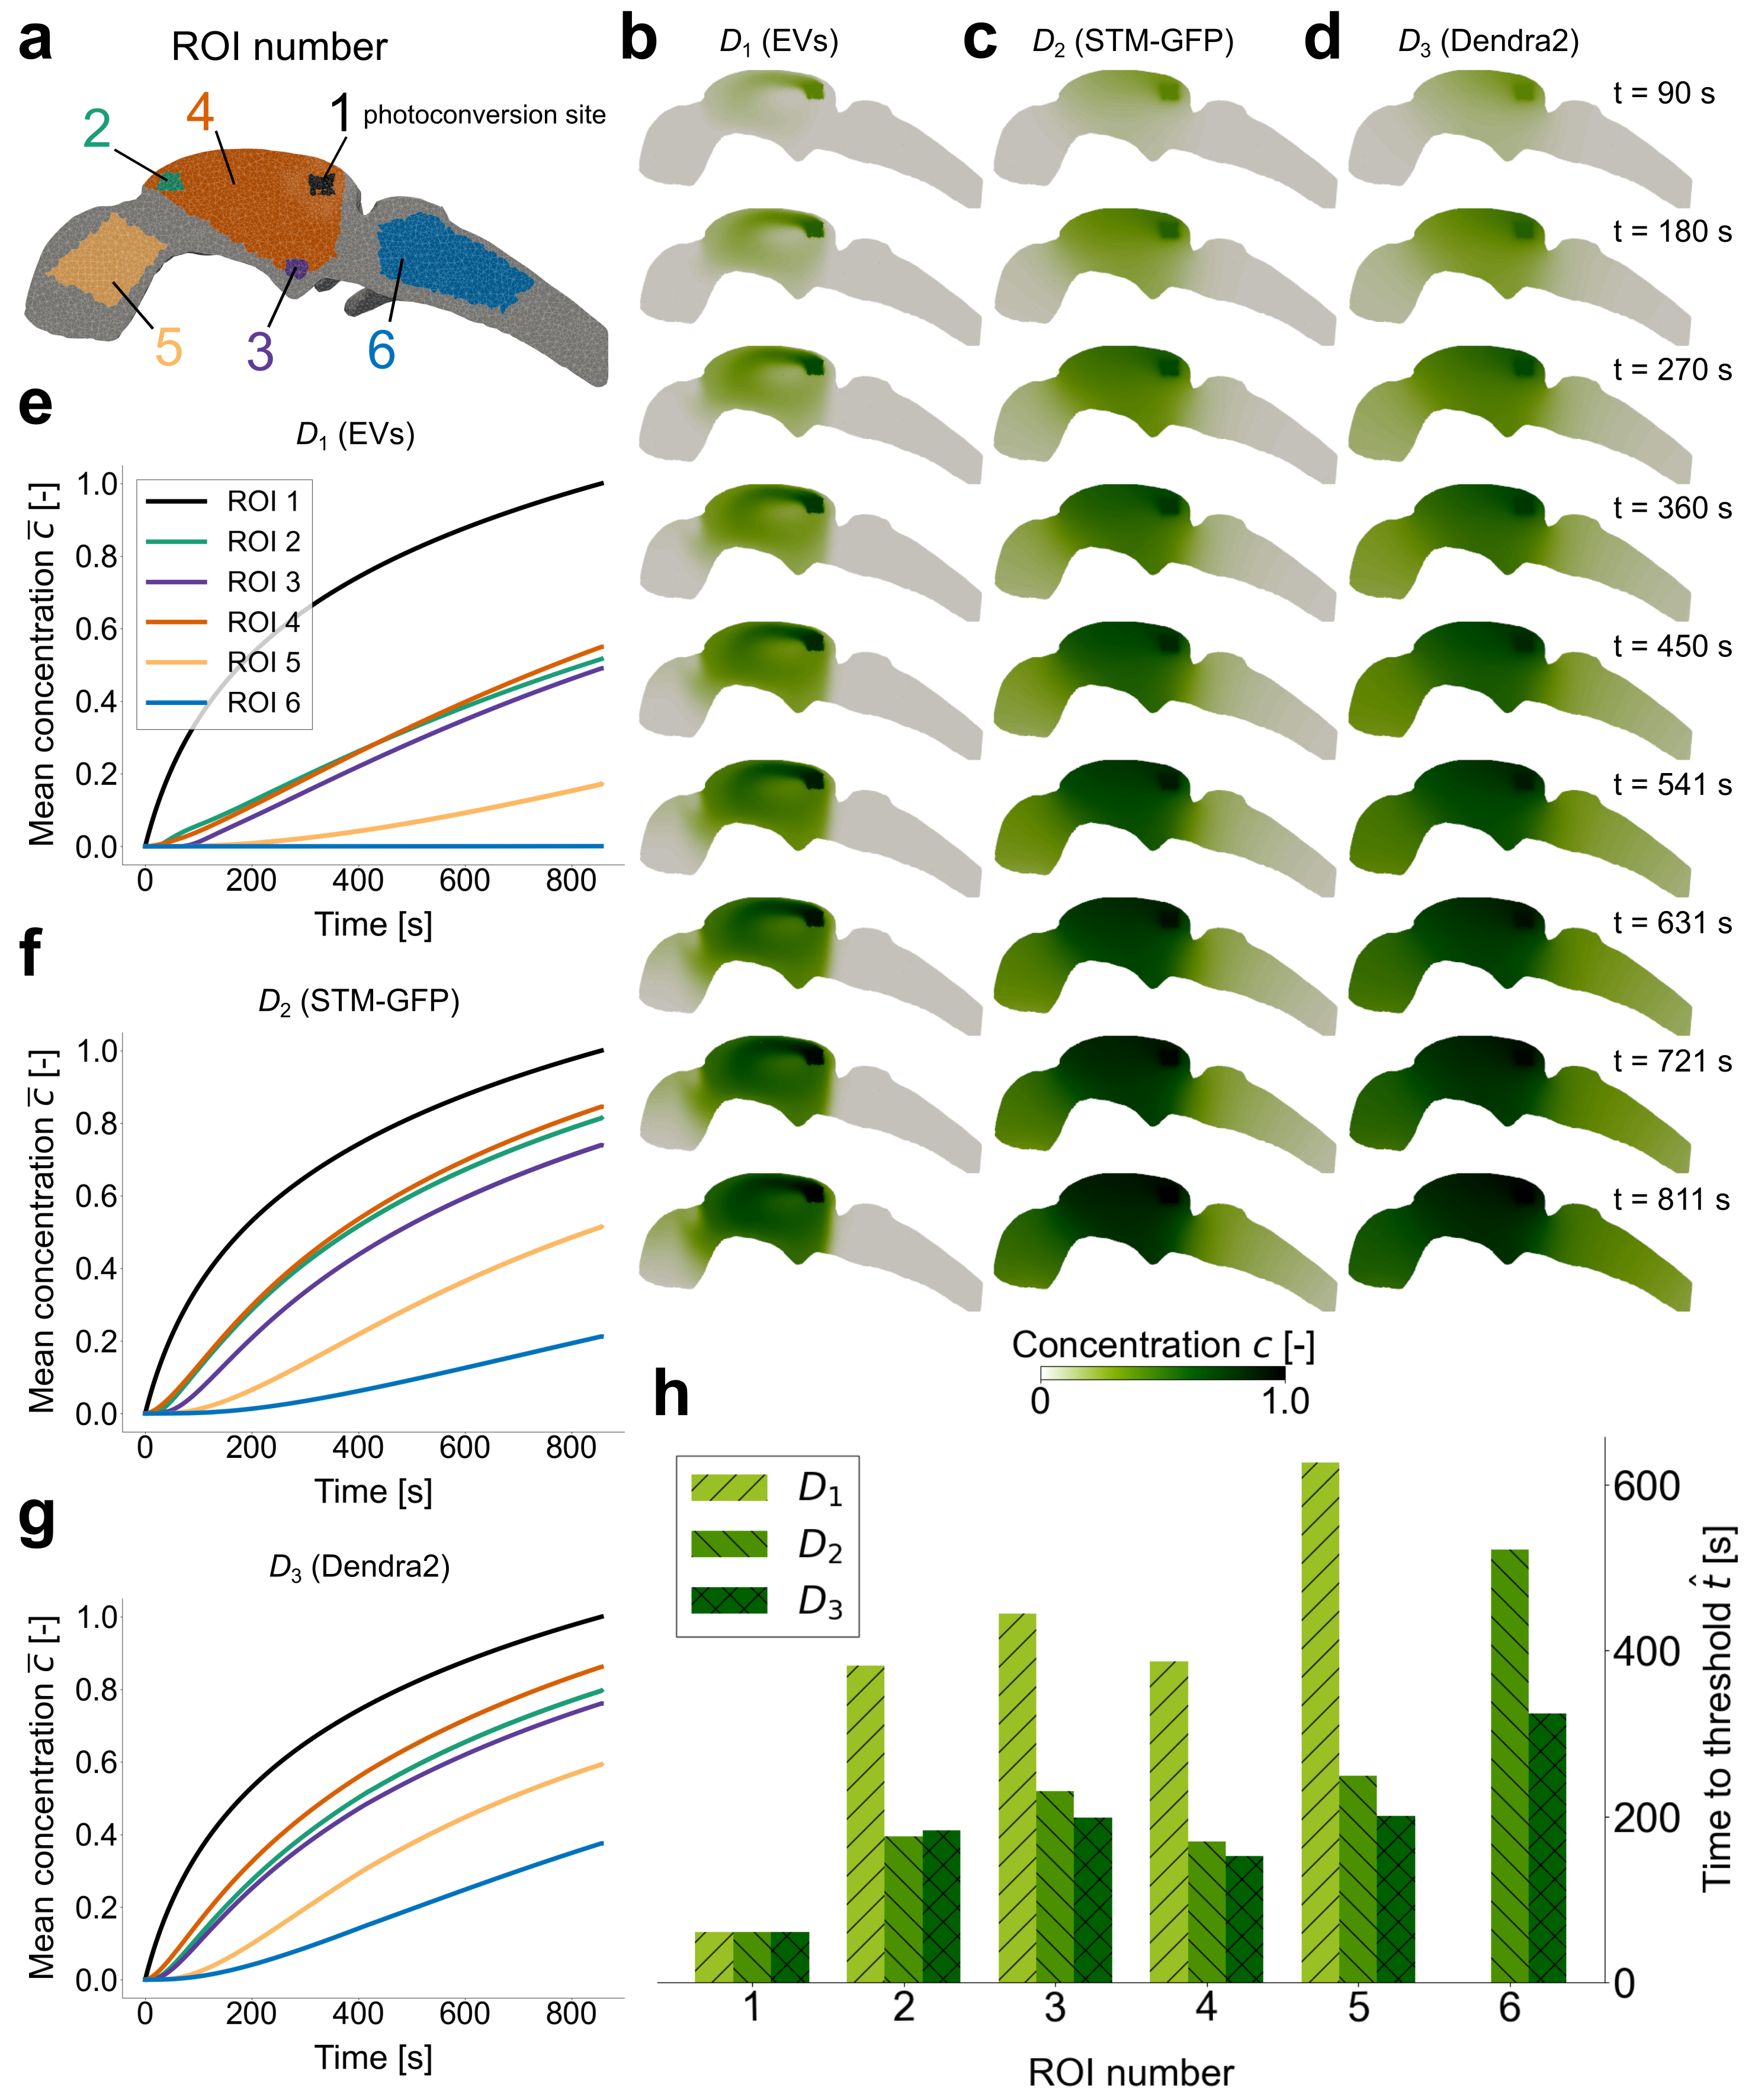
\includegraphics[width=0.95\textwidth]{graphics/figure2_simulation_results_different_coeffs.png}
    \caption{\textbf{a.} Slices in the $xz$-plane ($y=0.140$ mm, the center of the geometry) showing the concentration field simulated with diffusion coefficients $D_1$, $D_2$ and $D_3$ for three time instants $t=45.0$ s, $t=112.6$ s, $t=450.5$ s. Note that the colorbars indicating the magnitude of $c$ have different limits for each column. \textbf{b--d.} Mean concentration $\overline{c}$ in each region of interest (ROI) as function of time for diffusion coefficient $D_1$, $D_2$ and $D_3$, respectively. \textbf{e.} Geometry-centered clip of the ventricles mesh showing the locations of the ROIs. \textbf{f.} The time $\hat{t}$ before the mean concentration $\overline{c}$ exceeds a threshold value of $0.25$ (ROIs 2-4) or $0.10$ (ROIs 5, 6) in each simulation setup. Note that there is no bar for $D_1$ in ROI 6, because the threshold value was never exceeded.}
    \label{fig:figure2_compare_diffusion_coefficients}
\end{figure}

Transport of solute is quantified by the profile of the mean concentrations $\overline{c}_i(t)$ in the regions of interest (ROIs) $\Omega_i$ as functions of time~(\cref{fig:figure2_compare_diffusion_coefficients}, panels \textbf{b--d}).  An illustration of the ROIs is provided in \cref{fig:figure2_compare_diffusion_coefficients}, panel~\textbf{e}. The dynamics of ROI 1 follow from imposing~\cref{eq:injection_curve}. For ROIs 2--6, we observe more rapid concentration increases when the diffusion coefficient increases.  For all three diffusion coefficients, the dynamics of ROI 6 is the slowest. Region 5 exhibits a more rapid increase in mean concentration, and an even faster increase is observed for ROIs 2--4. The profiles of the latter three regions are similar, displaying only small differences in all of the three plots. \lyng{HH: Add some quantification in terms of percentages, e.g. final values of $\overline{c}_i$ for the different $D_i$?}
%\lyng{HH: is this really true?: Note that the total mass added to the system is not exactly the same for all three diffusion coefficients, since the total mass added depends on how fast the mass added in ROI 1 is transported away from that region.} 

We report the times $\hat{t}$ when the mean concentrations $\overline{c}_i$ first exceed a threshold value $\hat{c}$~(\cref{fig:figure2_compare_diffusion_coefficients}, panel \textbf{f}). Recall that $\hat{c}=0.25$ for regions of interest 1--4 and $\hat{c}=0.10$ for regions 5 and 6. The choice of different threshold values is because of the slower dynamics in ROIs 5 and 6. In region 6, the threshold is never exceeded for $D_1$, with the mean concentration close to zero at the end of the simulation. 

Finally, we calculate Péclet numbers for the entire ventricular geometry using estimates of the diffusion and advection timescales $t_d=L_p^2/D$ and $t_a=L_p/U_p$. Recall that
\begin{equation*}
    \mathrm{Pe} = \frac{\mathrm{diffusion \ timescale}}{\mathrm{advection \ timescale}} = \frac{t_d}{t_a},
\end{equation*}
so that if $\mathrm{Pe} > 1$, transport is dominated by advection, and if $\mathrm{Pe} < 1$ transport is dominated by diffusion. For the length scale $L_p$ we choose the approximate length of the ventricles geometry in the $x$-direction, $L_p=600 \ \mu$m. We use a mean velocity $\overline{U}$ as the characteristic velocity $U_p$. The mean velocity $\overline{U}$ is calculated by first averaging the velocity in space:
\begin{equation*}
    \overline{u}^2 = \frac{1}{|\Omega|}\int_{\Omega}\uu\cdot\uu\dx,
\end{equation*}
and then averaging $\overline{u}$ in time over one cardiac cycle to obtain $\overline{U}=1.41 \ \mu$m/s. This yields the three Péclet numbers $\mathrm{Pe}_1=519$, $\mathrm{Pe}_2=14.7$ and $\mathrm{Pe}_3=7.4$ for $D_1$, $D_2$ and $D_3$, respectively. \lyng{HH: move choice of length scale/calculation of velocity scale to Methods? Same question for Reynolds number calculation.} 

\subsection*{Comparing experimental and computational results}
Transport of photoconverted proteins is quantified by the change in fluorescence intensity $\Delta F=(F(t)-F_0)/F_0$ over time~(\cref{fig:figure3_compare_exp_and_sim_control}, panel \textbf{a}). The solid lines are the mean values of $\Delta F$ for the fish cohort, with shaded regions covering one standard deviation. The first region of interest (ROI 1) is the laser-targeted region. Qualitatively, the fluorescence intensity change in this region resembles intensity dynamics observed in experiments that studied the photoconversion properties of Dendra2 fluorescent proteins~\cite{Makarov2014Steady-stateDendra2}. The transport to the other regions can be separated into two groups: the fluorescence intensity change $\Delta F$ for ROIs 2--4 in the middle ventricle are all similar, whereas the more distal regions ROI 5 and 6 (anterior and posterior ventricle, respectively) exhibit a slower increase in $\Delta F$. In ROIs 2--4, the $\Delta F$ curves are concave, similar to ROI 1, while in ROIs 5 and 6 the curves are convex. Although the fluorescence intensity increases throughout all of the experiments, the maximum $\Delta F$ is not necessarily attained at the final time of the experiments. At the final time, the mean fluoresence intensities in regions 2--4 all exceed 0.60 (0.63, 0.71, 0.67, respectively) of the final value $F_0$ in ROI 1, wheras ROIs 5 and 6 reach mean values of 0.29 and 0.18, respectively.

% Final Delta F values
%0.6322650156762044 ROI 2
%0.7059449124175479 ROI 3
%0.6694500367160006 ROI 4
%0.28986700094045437 ROI 5
%0.18155055624229066 ROI 6

The experiment of photoconverting Dendra2 was simulated by solving the advection-diffusion equation with the diffusion coefficient $D_3$. We quantify the simulated transport with the time evolution of mean concentrations $\overline{c}$~(\cref{fig:figure3_compare_exp_and_sim_control}, panel \textbf{b}). Imposing the concentration in ROI 1 mimics the fluorescence intensity change $\Delta F$ in ROI 1. Since the initial condition of the simulation is a mean concentration of zero, the mean concentration $\overline{c}$ can be interpreted as the change in mean concentration and is thus a similar metric to $\Delta F$.

Comparing the simulation results with experimental results, transport dynamics of regions 2--6 are faster in the simulation. We observe higher final values of $\overline{c}$ compared to the final values of $\Delta F$ in the experiments. In simulations, the three $\overline{c}$ profiles of ROIs 2--4 behave similar as the $\Delta F$ profiles in these regions, although the orders of ROI 3 and 4 are opposite in the simulations as compared to the experiments. For all regions, the maximum mean concentration is attained at the final time of the simulations. The final value of $\overline{c}$ in regions 2--4 were 0.76, 0.72 and 0.82, respectively, compared to 0.63, 0.71 and 0.67 for $\Delta F$. As in the experiments, the transport to regions 5 and 6 is slower than the transport to the middle ventricle sites, though the final values of $\overline{c}$ are higher than those of $\Delta F$. The anterior ventricle (region 5) has a final $\overline{c}$ value of 0.56 (final $\Delta F= 0.29$), while in the posterior ventricle (region 6) the final value is 0.35 (final $\Delta F= 0.18$). Qualitatively, the $\overline{c}$ profile in the posterior ventricle compares with $\Delta F$ in this region, displaying a convex curve that has an approximately linear increase after an initial nonlinear increase. The anterior ventricle (region 5), on other hand, has an S-shaped $\overline{c}$ curve in the simulations, which differs from the linear $\Delta F$ curve in the experiments. 
% Final mean c values ROIs 2-6: 0.7637806  0.72025859 0.81903216 0.56204164 0.34926411
\begin{figure}[H]
    \centering
    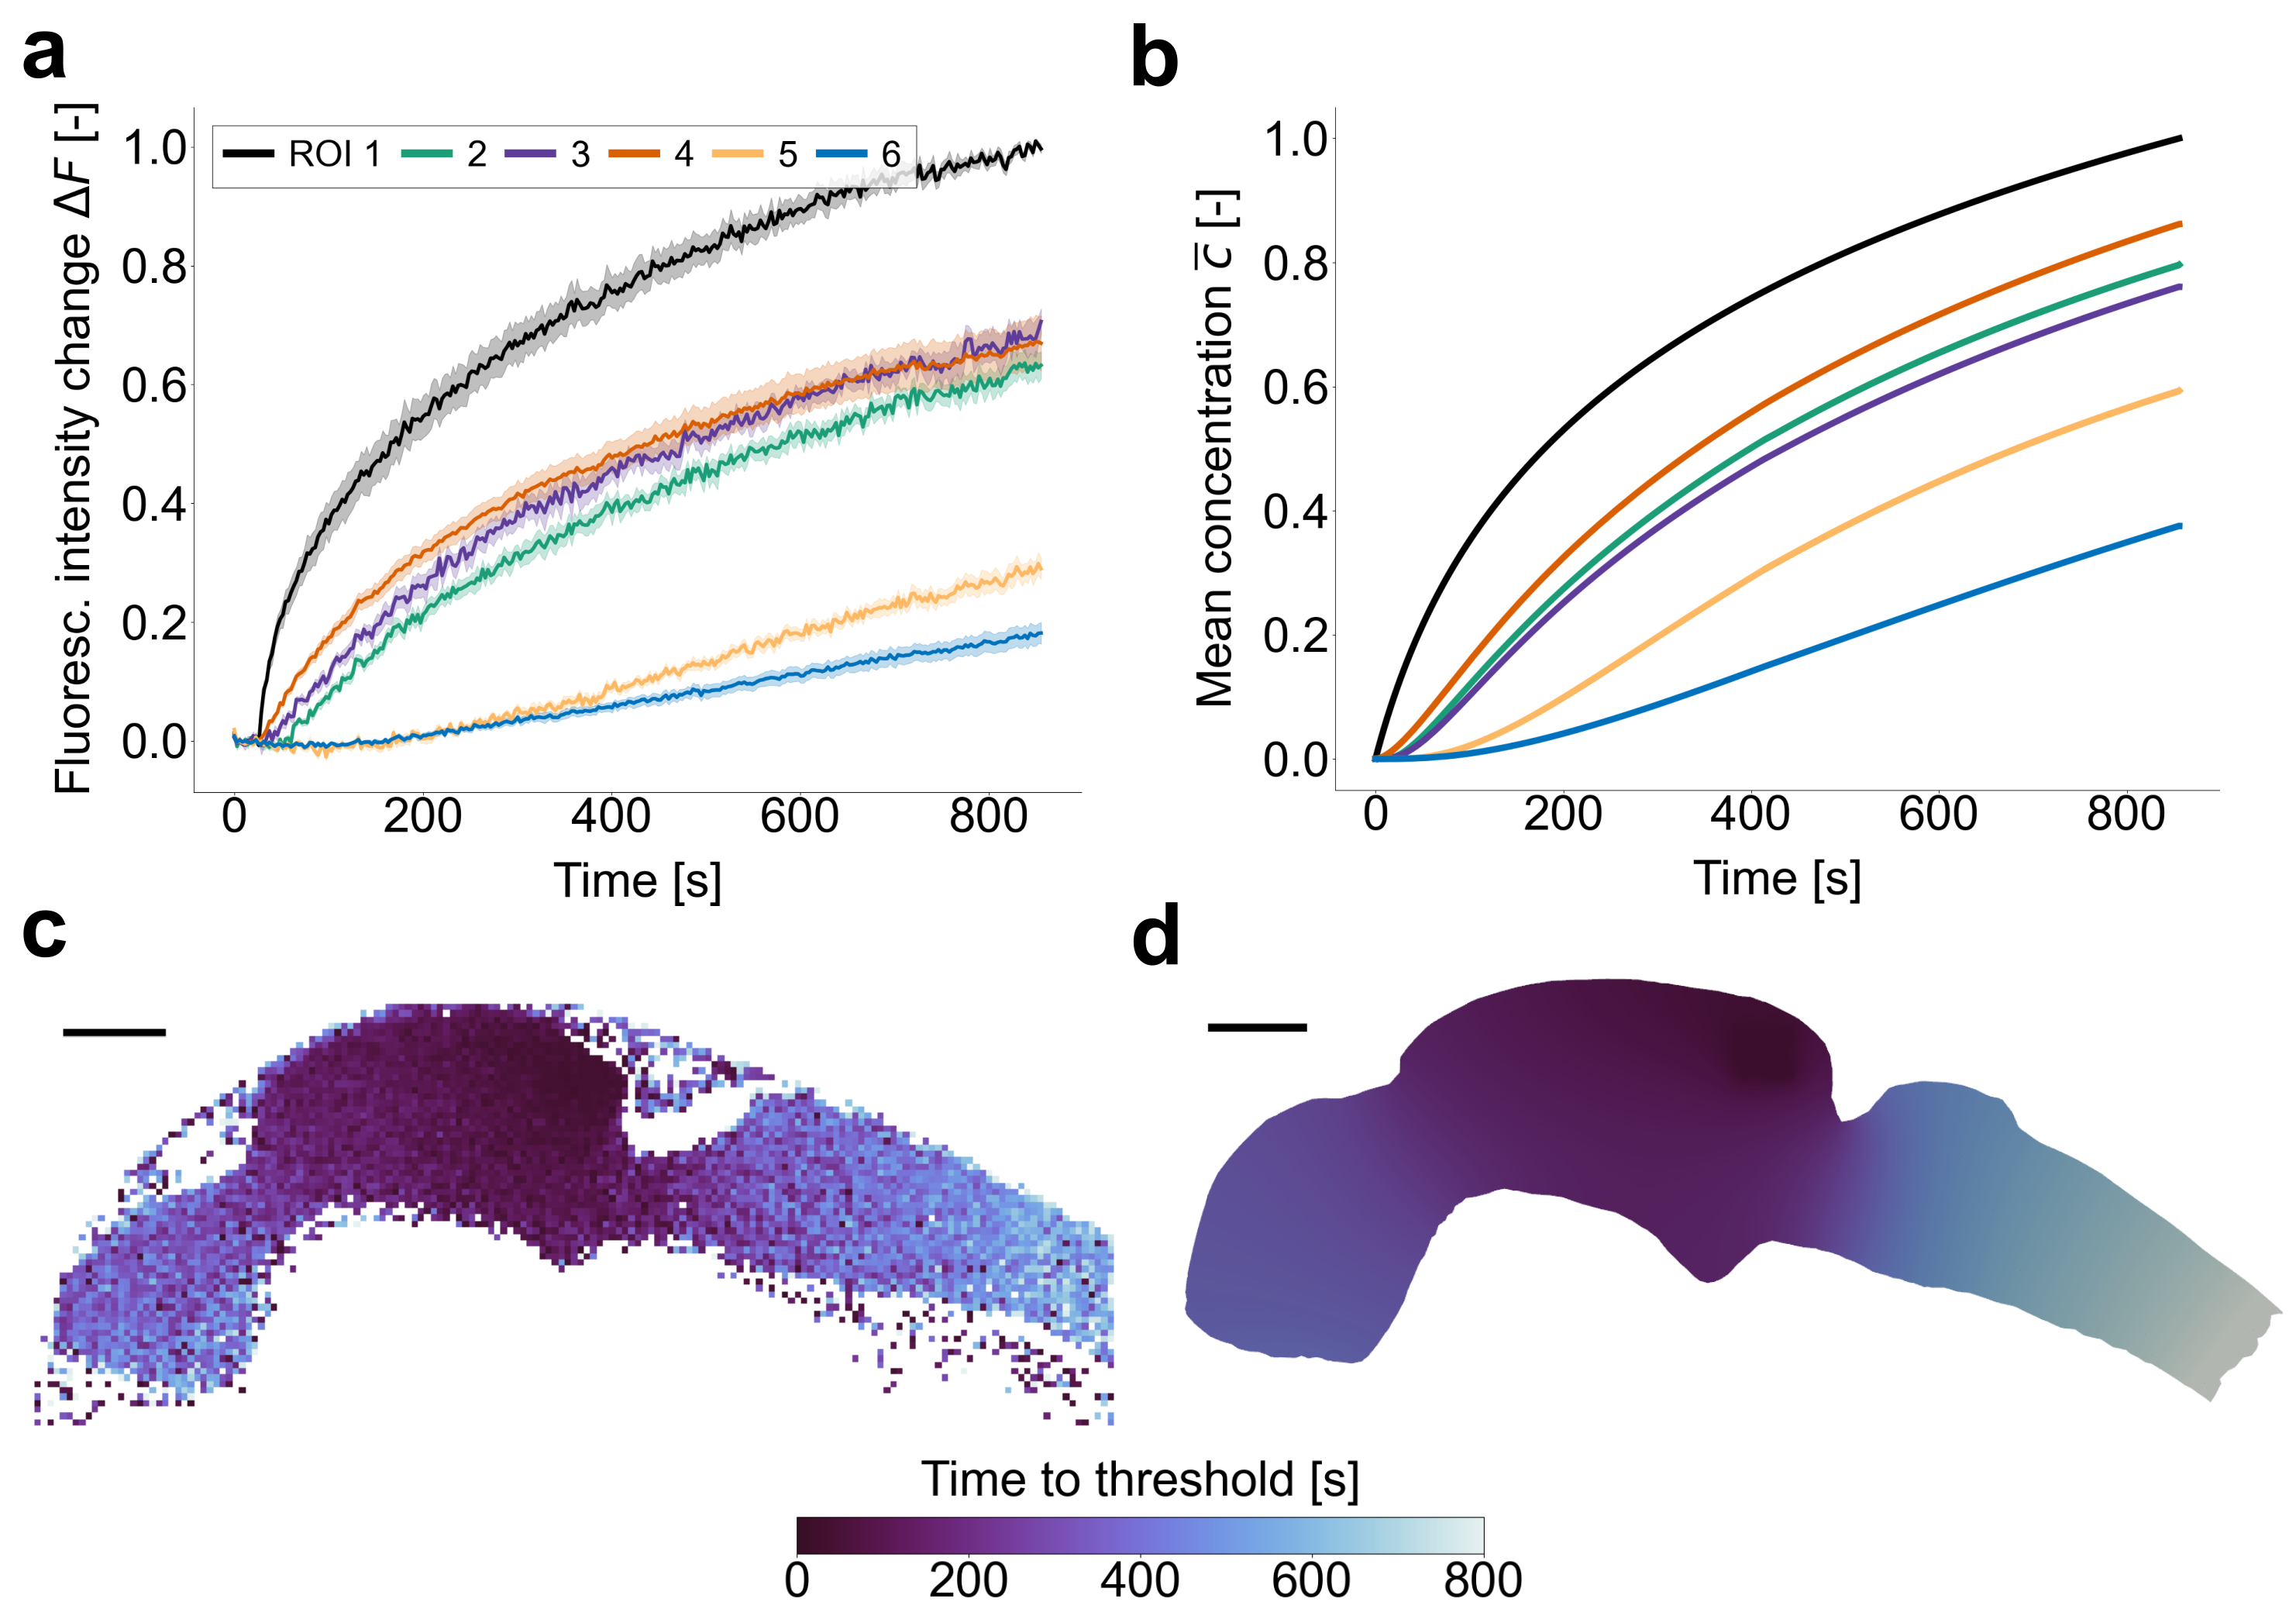
\includegraphics[width=\textwidth]{graphics/figure3_compare_experiments_and_simulations.png}
    \caption{\textbf{a.} Relative change in fluorescence intensity $\Delta F$ over time in each region of interest (ROI) observed during experiments of photoconversion of Dendra2 proteins in ROI 1. \textbf{b.} Mean concentration $\overline{c}$ as function of time in each ROI in a simulation of Dendra2 protein transport with the diffusion coefficient $D_3$. \textbf{c.} Time to $\Delta F$ reaches a threshold value of 0.25 in one of the animals of the dataset presented in panel \textbf{a}. \textbf{d.} Time to $\overline{c}$ reaches a threshold value of 0.25 for a transport simulation with diffusion coefficient $D_3$.}
    \label{fig:figure3_compare_exp_and_sim_control}
\end{figure}

We qualitatively compared fluorescence intensities and mean concentrations with the time $\hat{t}$ to exceed a threshold value of 0.25~(\cref{fig:figure3_compare_exp_and_sim_control}, panels \textbf{c} and \textbf{d}). For $\Delta F$, we determined this time-to-threshold for the same downsampled dataset that was used to calculate $\Delta F$. In the simulations, we determined the time for $\overline{c}$ to reach the threshold value in each degree of freedom of the concentration finite element function. We have excluded the posterior-most regions of the geometries in~\cref{fig:figure3_compare_exp_and_sim_control}, because the values of $\Delta F$ and $c$ never exceeded the threshold value of 0.25 in these regions. 

\subsection*{Absence of ciliary motion affects local protein distribution}
We compare the time evolution of fluorescence intensity in control and \emph{schmalhans}~(\emph{smh}) mutant zebrafish, plotting the means of $\Delta F$ across the cohorts, shaded with one standard deviation regions~(\cref{fig:figure4_compare_control_mutant}, panel \textbf{a}). Additionally, we determine the time needed to reach a threshold fluorescent intensity change in each region of interest (ROI) for each fish~(\cref{fig:figure4_compare_control_mutant}, panel \textbf{b}). It is important to note that this threshold was set differently for two groups of regions: the $\Delta F$ threshold value was set to 0.25 for ROIs 1--4, whereas for ROIs 5 and 6 the threshold value was 0.10. This choice was made because of the slower dynamics of ROIs 5 and 6. For each region of interest, the individual data points of the times to threshold are presented together with the distributions and the means of the data points. Based on the times to reach a threshold value of $\Delta F$, we test the null hypothesis that the control and mutant photoconversion data are from the same population (or equivalently, have equal distributions). We report the $p$-value for this hypothesis calculated using a two-sided Mann-Whitney U test that included a continuity correction, with a confidence level of 95\%. 

In ROI 2, there is a statistically significant slower fluorescence intensity increase in the \emph{smh} mutant fish compared to controls~(\cref{fig:figure4_compare_control_mutant}, panel~\textbf{b}). Compared to the control dataset, the mean time-to-threshold in ROI 2 is 45\% higher for the mutant dataset. In the other ROIs, the differences in the experimental results for controls and mutants are not significantly different. We observe that, both within the control and within the mutant dataset, there are considerable individual differences in the times to reach the threshold.

To simulate protein transport in mutant fish, we used flow model II (only cardiac motion as flow mechanism, no cilia) to model the ciliary dysfunction of the \emph{smh} mutants. We visualize the time evolution of the mean concentration $\overline{c}$ in each ROI for both model II and the baseline model (model 0), in addition to a similar time-to-threshold $\hat{t}$ as computed for the experimental data~(\cref{fig:figure4_compare_control_mutant}, panel~\textbf{c}). As for the experiments, we use a threshold value of $0.25$ in regions 2--4 and a value of $0.10$ for regions 5 and 6 to calculate $\hat{t}$. For ROI 2, we observe the same dynamics in simulations as in experiments: there is a slower increase in mean concentration in ROI 2 compared to the baseline model. The difference is even greater for the simulations, with the time-to-threshold in ROI 2 for model II 90\% higher than for model 0. Additionally, ROIs 4 and 5 exhibit very different $\overline{c}$ profiles for the two different flow models. The difference is less significant for ROI 3, and for the posterior ventricle (region 6) the profiles are very similar. 
\begin{figure}[H]
    \centering
    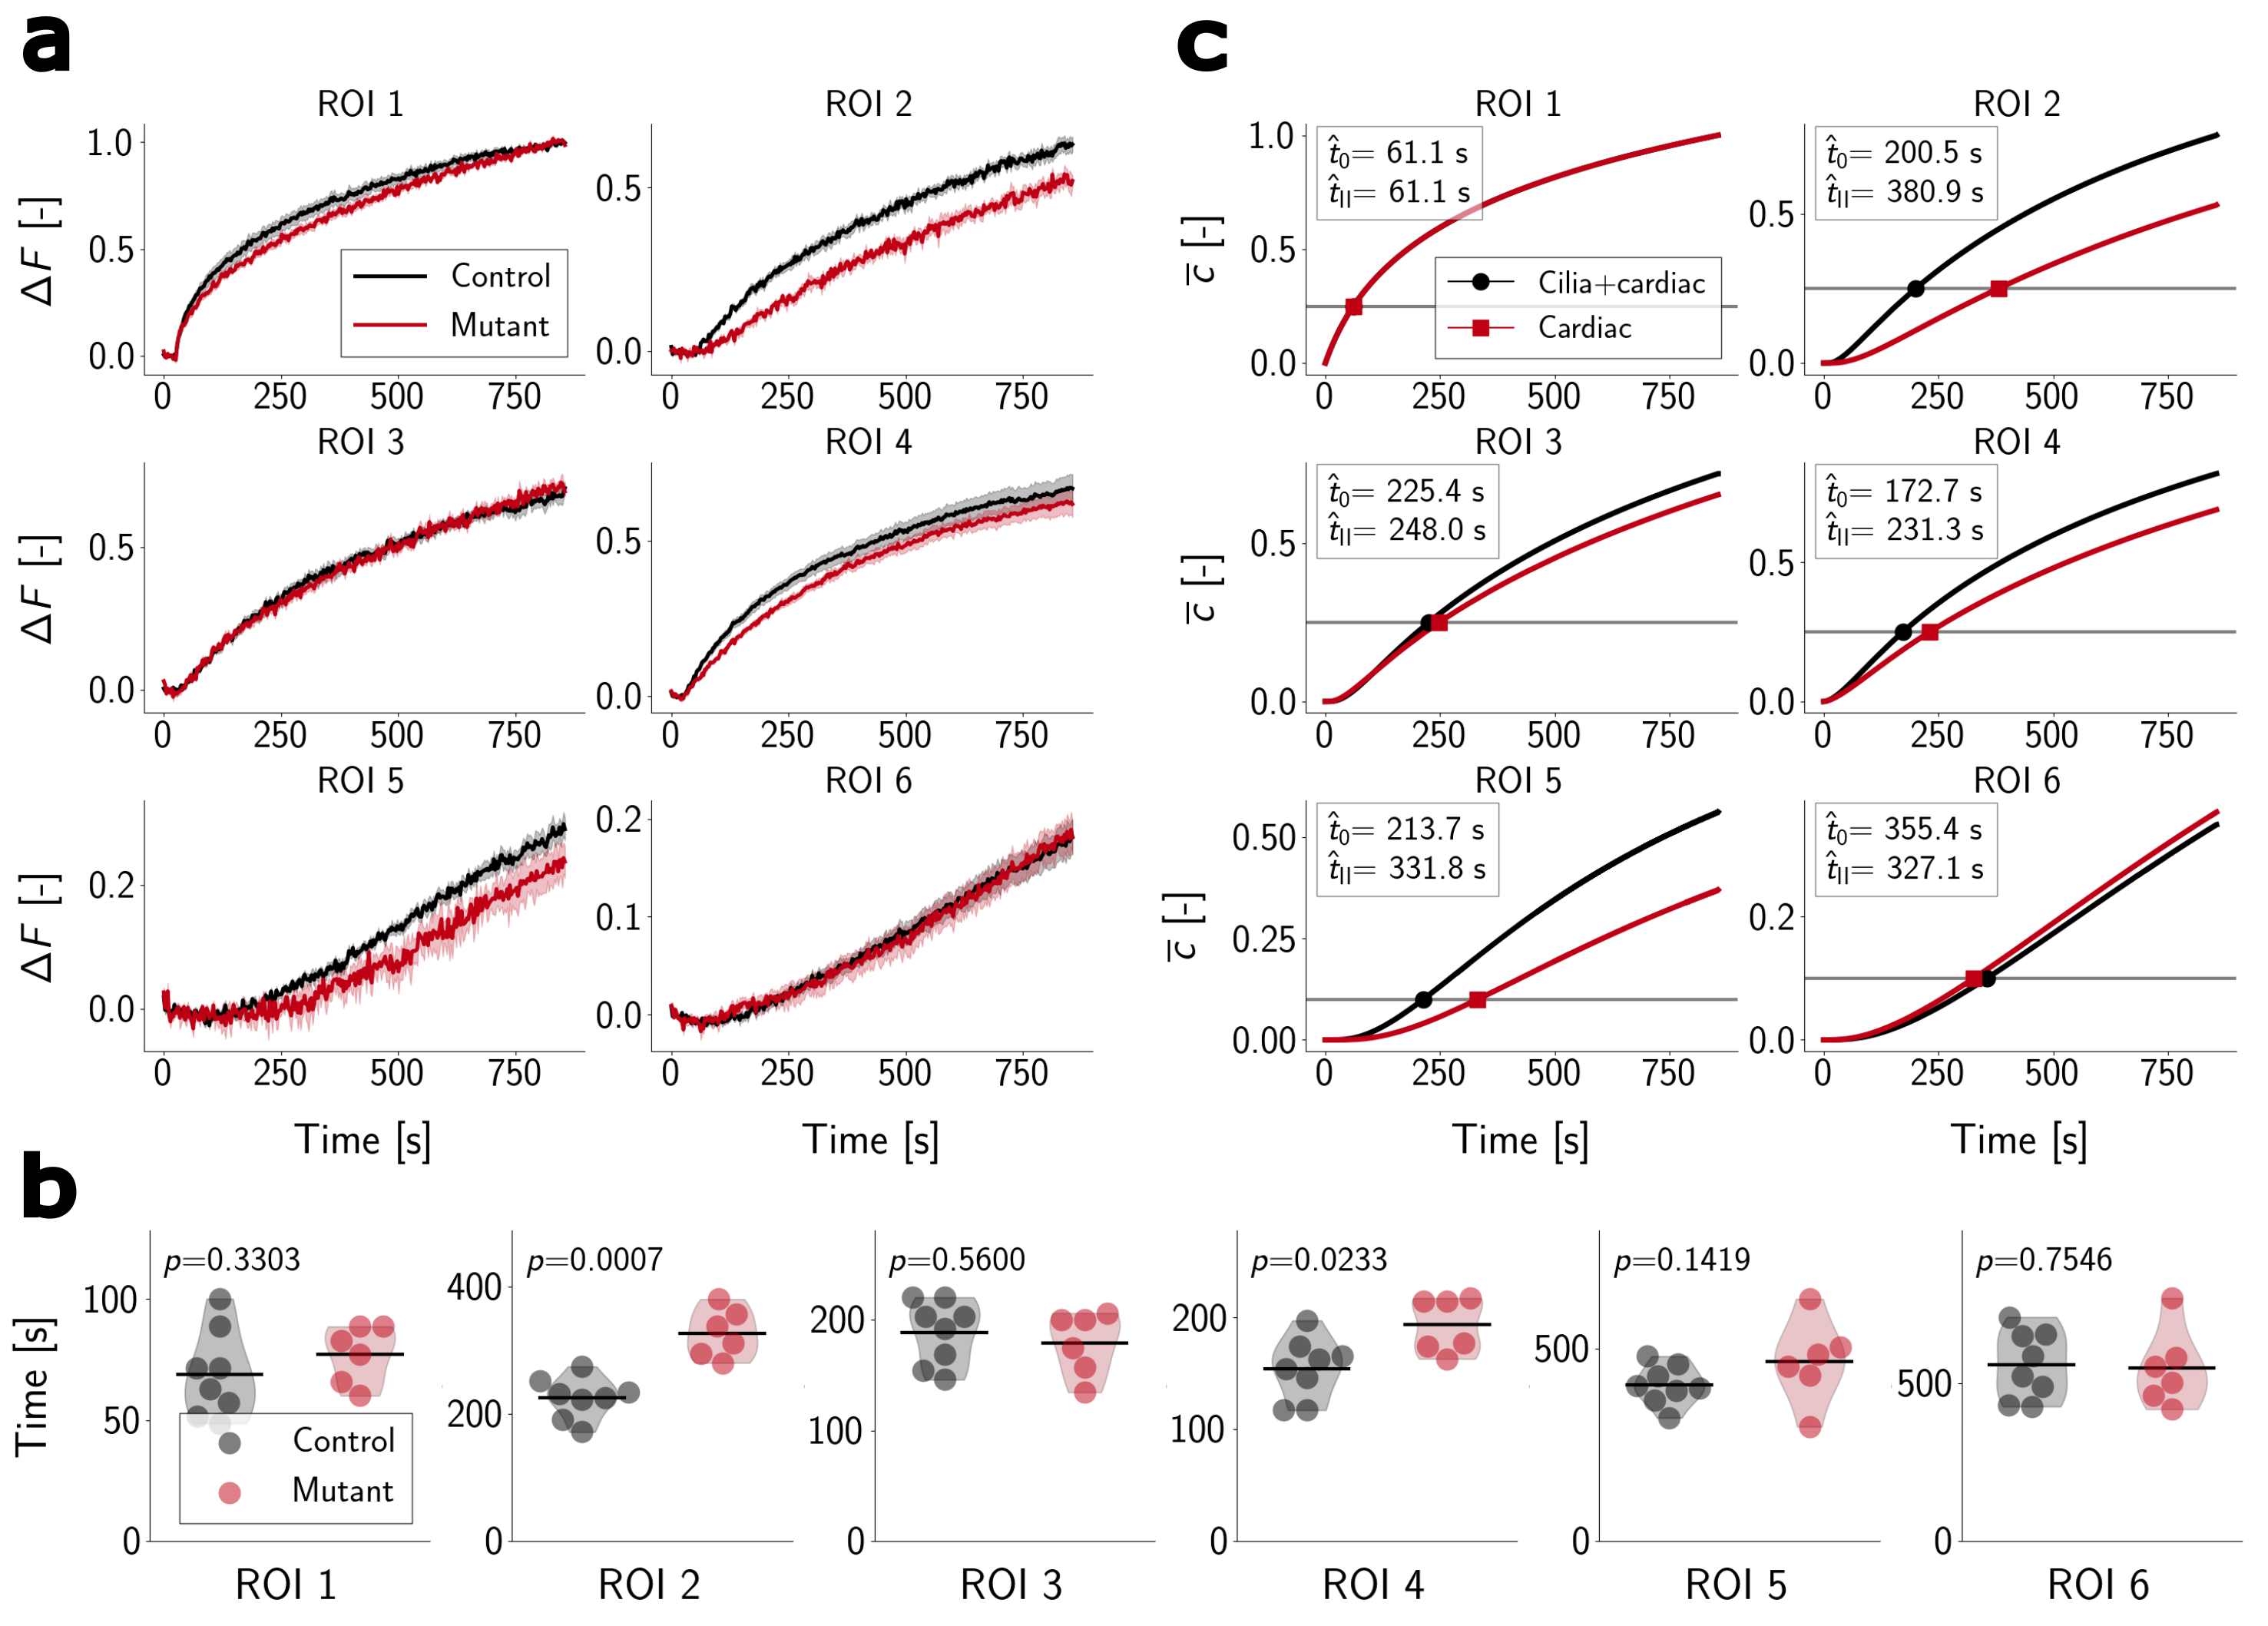
\includegraphics[width=\textwidth]{graphics/figure4_compare_control_mutant.png}
    \caption{\textbf{a.} Relative change in fluorescence intensity $F$ over time in each region of interest (ROI) for control (black lines) and \emph{smh} mutant (red lines) fish. 
    \textbf{b.} Times when $\Delta F$ first exceeds a threshold value, equal to 0.25 (ROIs 2-4) or 0.10 (ROIs 5, 6), for control (gray dots) and \emph{smh} mutant (red dots) fish. The thick black lines denote mean values of the datasets, and $p$-values were calculated using a Mann-Whitney U test with a confidence level of 95\%.
    \textbf{c.} Mean concentration $\overline{c}$ as function of time in each ROI, simulated using the baseline model (black lines) and the cardiac-only model (red lines). The horizontal gray lines mark the threshold value $\hat{c}$, and the time $\hat{t}$ when the threshold is first exceeded is reported in the plot legends. Note that in both panels \textbf{a} and \textbf{c}, the vertical axes have different limits in each plot.}
    \label{fig:figure4_compare_control_mutant}
\end{figure}

\subsection*{Loss of cilia can slow down transport}
Considering removal of cilia in three different regions through modified flow boundary conditions, we simulate CSF flow modeled by the Stokes equations and use the resulting velocity field in transport simulations of Dendra2. The maximum velocity observed in the simulations when removing telencephalic, ventral diencephalic and dorsal diencephalic cilia were, respectively, 27.7 $\mu$m/s, 27.2 $\mu$m/s, and 8.0 $\mu$m/s. We remind the reader that the maximum velocity observed for the baseline model was 27.7 $\mu$m/s.

Upon removal of telencephalic cilia, the evolution of the mean concentration $\overline{c}$ with time is essentially unaltered~(\cref{fig:figure5_compare_cilia_modifications}, panel \textbf{b}). Without ventral cilia in the diencephalic ventricle, $\overline{c}$ increases slightly slower in region of interest (ROI) 3 compared to the baseline model. Furthermore, there is a higher mean concentration in the anterior ventricle (ROI 5) and a lower mean concentration in the posterior ventricle (ROI 6) in the absence of ventral cilia when comparing to the baseline model, meaning more solute has spread towards the anterior ventricle and less solute has spread towards the posterior ventricle.

Changes in the transport dynamics are most prominent when removing the dorsal cilia in the diencephalic ventricle. For this setup, all ROIs (except ROI 1, for which we impose the concentration dynamics) exhibit significant changes in the dynamics of $\overline{c}$. Compared to the baseline model results, there is a slower increase in, and lower final values of, the mean concentration in middle and anterior ventricles (ROIs 2--5). In contrast, the transport to the posterior ventricle (ROI 6) is more rapid upon removal of the dorsal diencephalic ventricle cilia. It is evident from the final values of $\overline{c}$ that there is less total mass added to the system in the absence of dorsal cilia. \lyng{HH:This is due to the lower velocities in the vicinity of ROI 1, resulting in less ability to carry away mass from the volume where the concentration is imposed. \emph{Is this correct?}}
\begin{figure}[H]
    \centering
    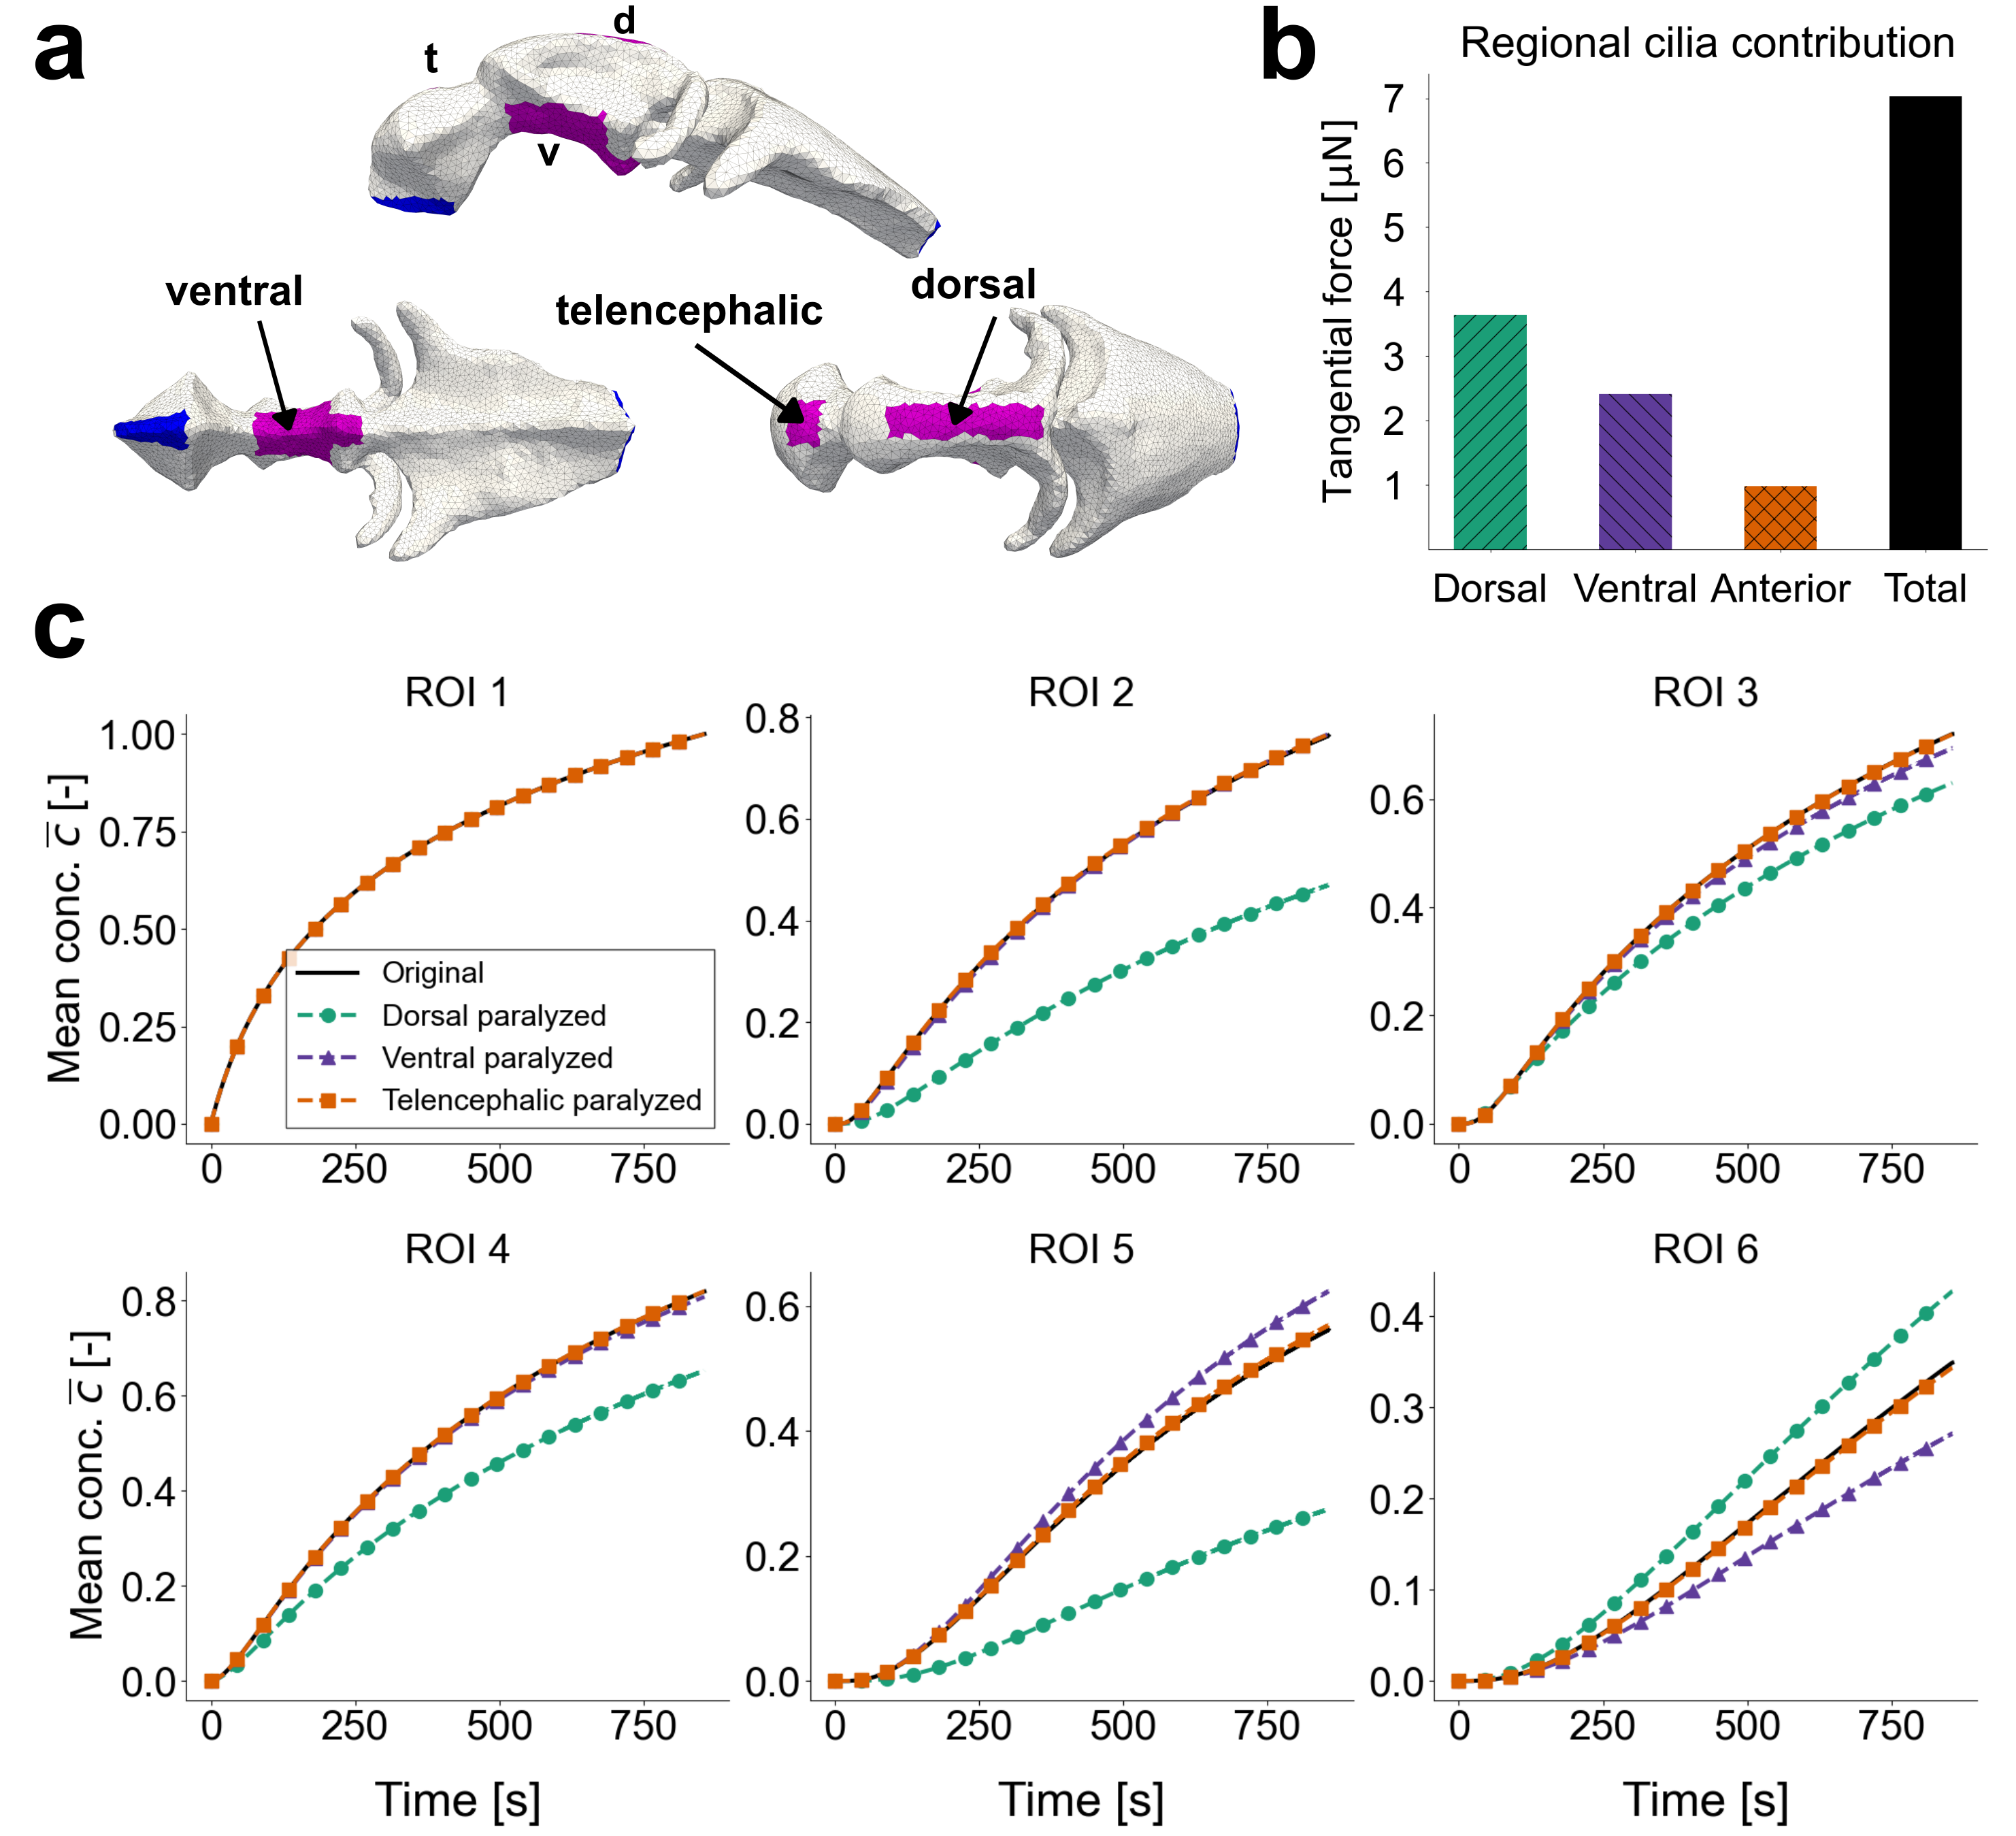
\includegraphics[width=\textwidth]{graphics/figure5_compare_cilia_modifications.png}
    \caption{Caption}
    \label{fig:figure5_compare_cilia_modifications}
\end{figure}

\subsection*{Modification of ventricles geometry impacts protein distribution}

The brain ventricular geometry varies significantly across zebrafish individuals, both healthy and sick animals. Motivated by an interest in how these variations can impact solute transport in the brain ventricles, we study the impact on simulation results when modifying the computational geometry and mesh in four different scenarios. Because our computational mesh is inflated by the dye-injection performed before image segmentation, we study four different mesh versions where we shrink: the fore-mid brain connection; the middle ventricle; the mid-hind brain connection; and all of the three above simultaenously. We used Blender~\cite{Community2018BlenderPackage} to modify the brain ventricles geometry.

We simulate flow and transport in four alternative brain ventricles meshes: one where the connection between the anterior and middle ventricles is constricted; one where the connection between the middle and posterior ventricles is constricted; one where the middle ventricle is shrunk in the lateral direction; the combination of the above three modifications~(\cref{fig:figure6_sim_results_compare_geometries}, panel \textbf{a}). We simulate CSF flow in the modified geometries with the baseline flow model and use the resulting velocity field to simulate transport of Dendra2.

Constricting the connection between the anterior and middle ventricle leads to slower transport to region of interest (ROI) 5 located in the anterior ventricle, and a slightly higher mean concentration in ROIs 2--4 and 6, compared to the original geometry. On the other hand, constricting the connection between the middle and the posterior ventricle leads to less transport into the posterior ventricle (ROI 6), and slightly more transport towards the anterior ventricle (ROI 5). Faster transport to ROI 5 and slower transport to ROI 6 is also the case for the geometry with a shrunk middle ventricle. Additionally, for this configuration the transport towards the anterior region of the middle ventricle (ROI 3) is slowed down. For the mesh where all three ventricles are modified, we observe higher retention of solute in the middle ventricles (ROIs 2--4). Both the anterior and the posterior ventricles (ROIs 5 and 6) have a lower mean concentration, compared to the results for the original geometry.

\lyng{HH: Quantify differences in terms of percentage changes in the final mean concentration values, maybe with a bar plot?}
\begin{figure}[H]
    \centering
    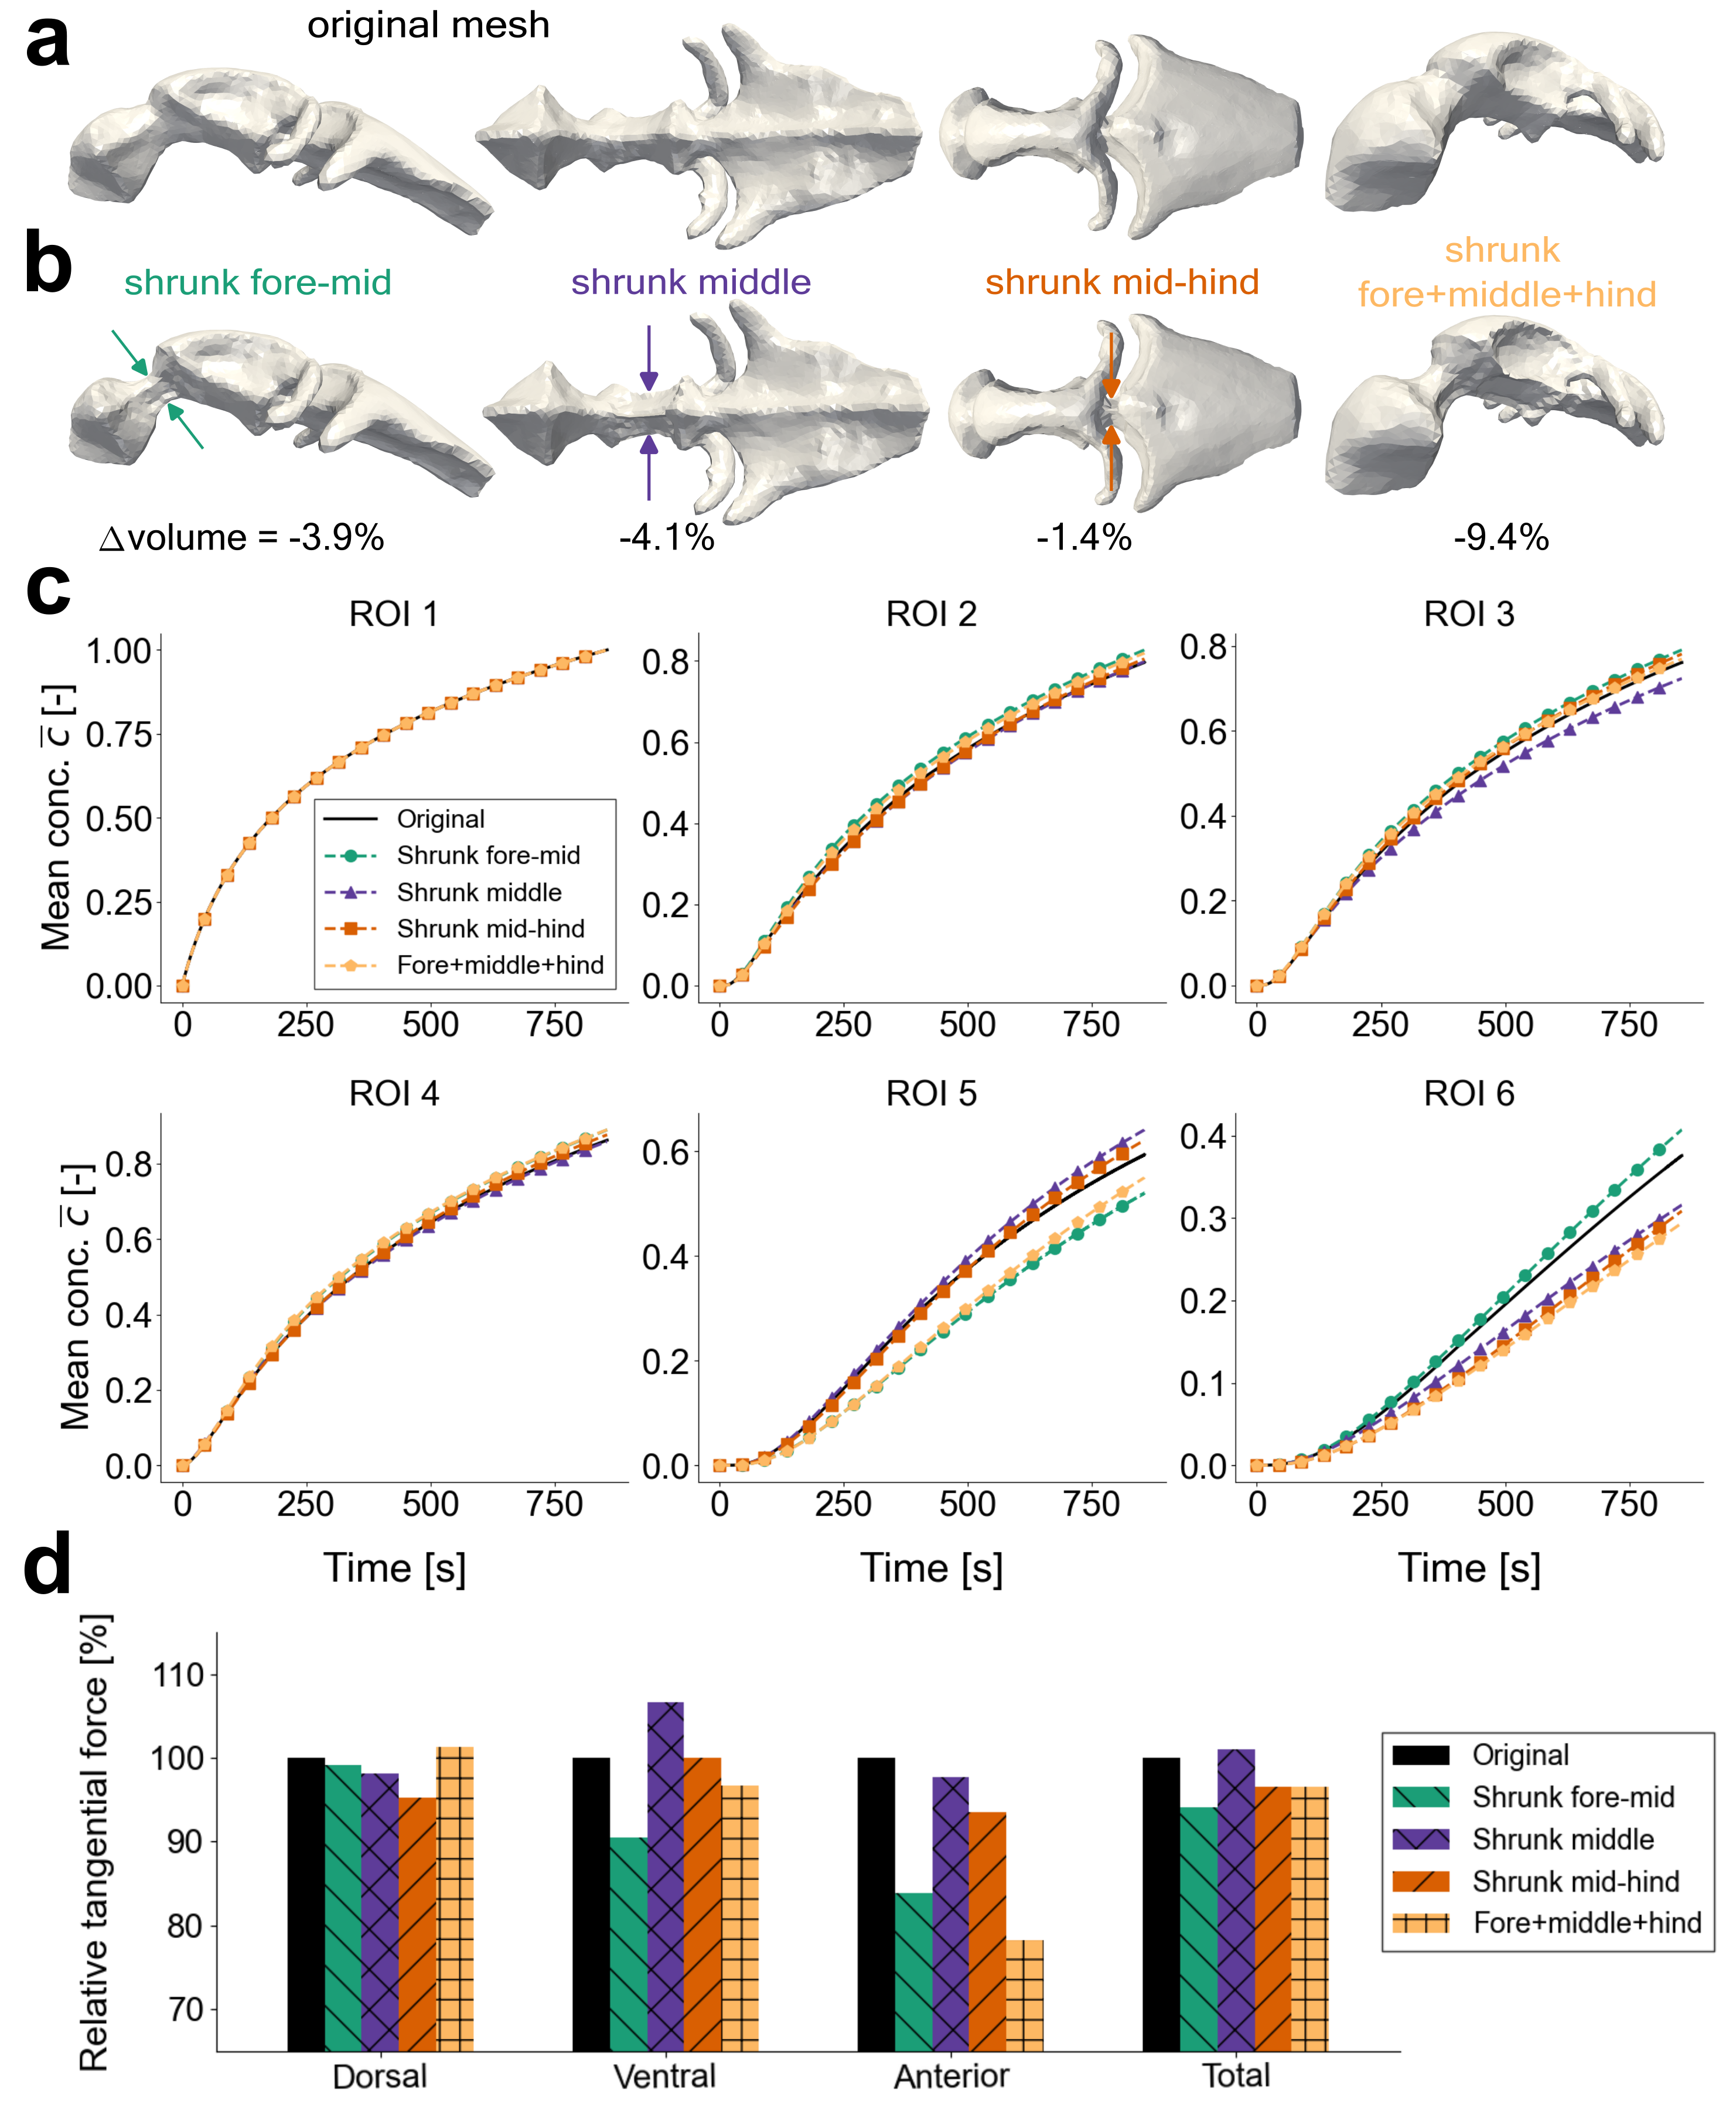
\includegraphics[width=\textwidth]{graphics/figure6_compare_modified_geometries.png}
    \caption{Caption. \mk{MK: How do the different geoemtries compare in terms of volume, areas where cilia are active?} \lyng{HH: Good question, will add this information.}}
    \label{fig:figure6_sim_results_compare_geometries}
\end{figure}

\cleardoublepage

%%--------------------------------------%%
%%--------------------------------------%%
%%--------------DISCUSSION--------------%%
%%--------------------------------------%%
%%--------------------------------------%%

\section*{Discussion}
We have presented a computational model of cerebrospinal fluid (CSF) flow in brain ventricles of 2 days post-fertilization (2dpf) zebrafish embryo. By imposing tangential stresses and normal traction on the CSF flow, the simulated flow fields had similar features to the flow fields observed experimentally, consisting of vortex-structured flow and pulsatile flow. The CSF flow was used to model transport of a solute by an advection-diffusion equation. Qualitatively, simulations compared well to experiments of Dendra2 fluorescent protein photoconversion. Transport in cilia-mutant fish (\emph{schmalhans} mutants) and a CSF model without cilia, was compared to control experiments and the baseline CSF model, indicating a local effect of cilia motion on protein transport. Using the computational model of flow and transport, we further studied region-specific removal of cilia and ventricles geometry modification, and how these changes affected transport.

\subsection*{The roles of diffusion and advection in transport of photoconverted proteins}
We quantified transport in terms of fluorescence intensity change $\Delta F$ (experiments) and mean concentration $\overline{c}$ (simulations) as functions of time. For both measures, we observed that transport dynamics in the middle ventricle where Dendra2 fluorescent protein was photoconverted contrasted with the dynamics of the more distal regions of the anterior and posterior ventricles. In experiments, regions distal to the photoconversion site showed an approximately linear increase in $\Delta F$, probably because advection is absent in the transport to the distal regions, such that diffusion is the sole mode of transport. In regions proximal to photoconversion, advection and diffusion occur simultaneously due to the presence of cilia, leading to concave profiles for $\Delta F$. The convex diffusion-only behavior was observed in the mean concentration $\overline{c}_6$ profile of the posterior ventricle in the simulations, but $\overline{c}_5$ was concave for the anterior ventricle, opposed to the experimental results \lyng{HH: \emph{Is this the correct interpretation of convex vs. concave curves?} Include some referencing to textbook solutions of the diffusion and advection equations to explain this convex vs. concave? E.g. semi-infinite slab or boundary layer solutions to inflow/outflow problem.}. Based on the geometry modification study, the reason for this difference in behavior might be that the duct between the anterior and middle ventricle is inflated in our computational mesh, as a result of the dye-injection performed before imaging~\lyng{Cite this?}. This inflation allows for effective cilia-mediated advection from the middle ventricle to the anterior ventricle.

In general, the mean concentration dynamics of the simulations was more rapid than the fluorescence intensity dynamics of the photoconversion experiments. This is strongly related to our definition of the photoconversion site (region of interest 1) in the simulations, and whether this corresponds well to the region used in experiments, because the volume of the photoconversion region used in the simulations determines the total amount of solute, and thus impacts the rate of transport. The alignment of the computational and experimental region of interest definition is hard to quantify. Additionally, a source of discrepancy in the results is the fact that the brain ventricles might be permeable, such that some Dendra2 diffuses out of the brain ventricles in the experiments. An assay has shown that the neuroepithelium lining the walls of brain ventricles in embryonic zebrafish 24 hours post-fertilization is permeable to dyes smaller than 70 kDa~\cite{Chang2012AnNeuroepithelium}. Dendra2 are almost 26 kDa in size~\cite{Gurskaya2006EngineeringLight}, and are thus under this reported limit. If such permeability also is the case for 2 days post-fertilization zebrafish embryo ventricles, this would lead to Dendra2 leaking out of the brain ventricles in the experiments, making the dynamics appear slower. 

Transport of Dendra2 fluorescent protein appears to be a balance of advection and diffusion. Advection is the strongest transport mechanism on a global scale (global Péclet number 7.4), but for shorter distances diffusion is balancing out advection. Simulating transport of larger molecules (thus with smaller diffusion coefficients) proved advection to be increasingly important as molecule size increased. For the smallest diffusion coefficient used, $D_1$, which represented 200 nm exosomes, there was essentially zero solute in the posterior ventricle at the final simulation time (around 850 s). This is consistent with the statement above that transport to the posterior ventricle from the middle ventricle is driven by diffusion, based on estimated transport times of diffusion and advection: For $D_1$, an estimate of the diffusion timescale $t_d=L^2/D_1$ over a distance $L=200$ $\mu$m from the middle to the posterior ventricle is approximately 24500 s. Advective transport by the mean velocity $\overline{U}=1.41 \ \mu$m/s over the same distance would happen on a timescale of the order of $t_a=L/\overline{U}=141$ s. Comparing this with the minuscule values of $\overline{c}_6$ after simulating transport with $D_1$ for 850 s, one can conclude that if advection played a role in transporting solute from the photoconversion site in the middle ventricle to the posterior ventricle, values of $\overline{c}_6$ would be higher than those observed.

The changes in the times to threshold when changing the diffusion coefficient are greatest for regions of interest (ROIs) 4--6, further indicating that, relative to advection, diffusion has a greater impact in these regions than compared to regions 1--3. In region of interest 2 (anterior, dorsal region of the middle ventricle), the time to threshold is lower for $D_2$ than $D_3$. This is probably a result of less solute diffusing away from ROI 1 for $D_2$ than for $D_3$, meaning that more solute can be transported by advection along the ciliated walls of the ventricles towards ROI 2. We also note that, for regions of interest 3 and 4, the order of the $\Delta F$ and $\overline{c}$ profiles are opposite. This could be related to the difference in the exact location of ROIs 3 and 4 in simulations and experiments, or due to cilia-advection being more prominent in the simulations (cf. the discussion on differences in transport to the anterior ventricle).

\subsection*{Simulation studies: modifying cilia and geometry}
We studied the impacts of removing cilia in specific regions of our model~(\cref{fig:figure5_compare_cilia_modifications}). Removing the dorsal cilia has a strong impact on the resulting CSF flow field and the mean solute concentration. Removing the dorsal cilia decreased the maximum velocity in the ventricles roughly by a factor of three from 27.7 $\mu$m/s to 8.0 $\mu$m/s. The impactful changes to the flow field is because the total force applied on the dorsal cilia boundary is great in magnitude in our model, and the dorsal cilia are thus important to establishing the CSF flow structures. With weaker flow in the dorsal region of the middle ventricle, there is less advective transport. \lyng{HH: Quantify the difference in force applied in the dorsal region: $\int_{c, dorsal}\btau\cdot\mathbf{t}\,\mathrm ds$.}

Absence of ventral cilia in the middle ventricle did not greatly impact flow dynamics and transport, but lead to slightly less transport towards the posterior ventricle, and slightly more transport towards the anterior ventricle. This is because the ventral cilia help induce flow towards the posterior ventricles. Removing the cilia in the anterior ventricle leaves the transport results virtually unaltered, although the CSF flow vortex structure in the anterior ventricle vanishes. This would then probably have a greater impact for smaller diffusion coefficients, as it is evident in~\cref{fig:figure2_compare_diffusion_coefficients} that transport with $D_1$ is mainly advective.

\lyng{HH: Compare numerical results with transport results in Figure 7 in \cite{Olstad2019CiliaryDevelopment}.}


\lyng{HH: Discuss cilia serving as an "enhanced mixing factor" on small scales, refer to this~\cite{Siyahhan2014FlowVentricles} and this~\cite{Yoshida2022EffectVentricles} paper that studied this in human brain ventricles. Include a discussion of what happened when these papers removed cilia.}

Modifying the ventricular geometry had varying impact on transport~(\cref{fig:figure6_sim_results_compare_geometries}). Both when (separately) shrinking the connection between the fore- and mid-brain and the mid- and hind-brain, we observe a slight increase in the mean concentration $\overline{c}$ of regions of interests 2--4. In regions 5 and 6, we observe a decrease in $\overline{c}$ in the region that we shrink the connection from the middle ventricle to. Meanwhile, the other region has an increase in $\overline{c}$, a result of mass conservation. When shrinking the middle ventricle, the mean concentration decreases in regions 2--4. The effect on $\overline{c}$ in regions 5 and 6 is similar to when the mid-hind connection is shrunk: less solute is transported towards the hind-brain and more solute is transported towards the fore-brain. 

Combining all three geometry modifications, we see an increase in $\overline{c}$ in regions 2--4. Now, there is a decrease in both region 5 and 6, which is more similar to the experimental $\Delta F$ curves (\cref{fig:figure3_compare_exp_and_sim_control}, panel \textbf{a}) in these regions compared to the simulated $\overline{c}$ on the standard geometry (\cref{fig:figure3_compare_exp_and_sim_control}, panel \textbf{b}). This is in line with the expectation that shrinking the geometry is closer to replicating the geometries of the fish used in experiments, because the ventricular geometry is inflated by the injection procedure performed during image segmentation.

\subsection*{Computational model assumptions and boundary conditions}
To model flow of cerebrospinal fluid, we employed slip boundary conditions at the ventricular walls, contrasting the classical choice of a noslip boundary condition. The use of slip boundary conditions is motivated by experimental observations of the flow field in zebrafish embryo brain ventricles~\cite{Olstad2019CiliaryDevelopment}. It has been observed that the fluid velocity increases towards the wall~(this is also evident in~\cref{fig:figure1}, panel~\textbf{c}). Using slip boundary conditions allows for this behavior. A couple of previous continuum model simulation studies of cilia-mediated flow~\cite{Siyahhan2014FlowVentricles, Thouvenin2020OriginCanal} have modeled cilia as body forces. We chose to model the cilia as a force exerted tangentially on the boundary. First, we deem this a good representation of the real nature of cilia, since they are in reality microscale structures confined to the ventricular walls that generate flow through collective motion. Second, it avoids the need of excessive mesh refinement near the ciliated boundaries in the case that a body force were to be applied in a $\sim$ 5 $\mu$m~\cite{Salman2022ComputationalEmbryo} deep cilia layer.

In our CSF flow model, the ciliated boundaries are homogeneous, whereas in reality, cilia populate the ventricle walls in a heterogeneous manner~\cite{Olstad2019CiliaryDevelopment}. Heterogeneous spatial arrangement of cilia, both in location and beating direction, has been shown to enhance particle clearance in airway cilia arrays in mice~\cite{Ramirez-SanJuan2020Multi-scaleArrays}. Incorporating spatial arrangement heterogeneity in our model could possibly result in different transport timescales, but we would not expect notable changes to the general trends of the macroscopic transport that we study here, since the effects of introducing heterogeneous spacing of cilia would alter the magnitude of cilia forces, but not their direction. On the other hand, introducing more heterogeneous beating directionality could alter the transport timescales as well as the directionality. In our model, all of the applied cilia tangential traction is aligned with the rostrocaudal axis, and more heterogeneity in this alignment to reflect heterogeneity in the beating directionality of cilia would presumably affect both magnitude and directionality of advective transport. Previous studies have demonstrated that changes to beating directionality affects transport, and that specific coordination of the ciliary beating is important in the brain ventricles for flow and signaling processes~\cite{Eichele2020Cilia-drivenVentricle, Olstad2019CiliaryDevelopment, Faubel2016Cilia-basedVentricles, Guirao2010CouplingCilia, Afzelius2004Cilia-relatedDiseases}, but also in other phenomena such as maintaining healthy functioning of mucous transport in airways~\cite{Rayner1996CiliarySyndrome, Schneiter2021Multi-scaleFunction, Bustamante-Marin2019LackClearance, Tsukita2012CoordinatedFeet} and in nodal flow which establishes left-right symmetry in mammals~\cite{Yoshiba2014RolesSymmetry, Hirokawa2006NodalAsymmetry, Sawamoto2006NewBrain}. Although these studies were mostly on spatial scales resolving individual cilia, we could envision the same effects in our continuum model, similar to the results of previous numerical studies~\cite{Ramirez-SanJuan2020Multi-scaleArrays, Thouvenin2020OriginCanal, Yoshida2022EffectVentricles}. 

We used an advection-diffusion equation to simulate protein transport in the brain ventricles. Except for where we imposed a normal pressure boundary condition on the CSF flow, we imposed a no-flux condition on the concentration. Imposing a pressure-driven cardiac-related flow on certain parts of the CSF flow boundary leads to in- and outflow, and the advective transport then requires handling of in- and outflux boundary conditions. Reflecting our assumption that the ventricular system is closed, we set boundary conditions such that the total mass is conserved in the limit that the timestep size is zero. We handle the outflux by leaving the advective flux term as an unknown in the weak formulation of the advection-diffusion equation. This has been referred to with different names in previous works, names such as the ``free boundary condition"~\cite{Papanastasiou1992ACondition}, the ``no boundary condition"~\cite{Griffiths1997TheCondition}, and the ``consistent flux boundary condition"~\cite{Lynch2020NumericalHemodynamics}. In leaving the advective flux term in the weak form we are lacking a boundary condition, so the approach seems problematic in the continuous sense of the problem. However, the discrete problem is well-posed, because the approach represents constraining higher-order derivatives of the concentration~\cite{Griffiths1997TheCondition}. 

On the inflow boundary, we applied an approximate periodic boundary condition by setting the inflow boundary flux at timestep $n$ equal to the outflow boundary flux at the previous timestep $n-1$. This is expected to be of low-order accuracy, and for high Péclet numbers, the boundary condition affects the concentration field in the vicinity of the in- and outflow boundaries due to large advective fluxes. For the simulation scenarios we considered, both in terms of model parameters and time span, the photoconversion region where solute originates is far enough away from the in- and outflow boundaries for the flux boundary condition to not significantly impact the results. Nevertheless, we deliberately excluded the space proximal to in- and outflow boundaries in the anterior and posterior regions of interest (5 and 6) to limit adverse effects. 

A possible improvement to the in- and outflow boundary conditions we employed would be to consider a 3D-0D coupling of the in- and outflow boundaries using ordinary differential equations, similar to what has been done in cardiac modeling~\cite{Brown2024AMechanics, Augustin2021ACirculation}. However, if the ventricular system in reality is a closed system, one should rather seek out a way of modeling the CSF flow without open boundaries to avoid handling in- and outflow boundary conditions. A more appropriate way of handling the beating cardiac motion could be to impose a ventricular wall deformation, assumed to result from pulsatile motion of the heart and/or cardiac vessels surrounding the ventricles. This wall deformation would induce CSF flow while simultaneously permitting enforcement of the impermeability condition $\uu\cdot\nn=0$ on the ventricular walls. Such wall-motion induced CSF flow has been modeled and simulated successfully in the human brain ventricular system~\cite{Causemann2022HumanFramework, Kurtcuoglu2005ComputationalSystem, Kurtcuoglu2007ComputationalSylvius, Linninger2005PulsatileBrain}.

\subsection*{Estimation of computational model parameters}
The diffusion coefficients used in this study were partially based on values from experiments and partially estimated. The value $D_3=\num{1.15e-10} \ \mathrm{m^2/s}$ is based on the value $\num{1.15e-10} \pm 0.11 \ \mathrm{m^2/s}$ reported in an experiment~\cite{GuraSadovsky2017MeasurementExpansion}, while the values $D_2$ and $D_1$ were extrapolated based on experimental data~\cite{Swaminathan1997PhotobleachingDiffusion, Potma2001ReducedCells, Mahmood2023ExosomeTemperature} using the Stokes-Einstein relation~\cite{Einstein1905UberTeilchen}~(\cref{eq:D_stokes_einstein}). This extrapolation assumes the diffusing substance is of spherical shape, which proteins are not, and the relation does not necessarily hold in CSF. Consequently, there is uncertainty in the values used. We note that Sadovsky~\emph{et al.}~\cite{GuraSadovsky2017MeasurementExpansion} reported that Dendra2 satisfies the Stokes-Einstein in the solution they used, a solution which had similar viscosity to water. We used CSF density and viscosity values measured in humans~\cite{Bloomfield1998EffectsFluid}, and because embryonic CSF in zebrafish is high in proteins, nutrients and other substances, the CSF in which photoconverted Dendra2 are transport in our experiments may be more viscous than what we consider. This would reduce the diffusion coefficient~(cf.~\cref{eq:D_stokes_einstein}), but based on reports of protein concentration having a limited impact on the viscosity of CSF~\cite{Bloomfield1998EffectsFluid, Brydon1995PhysicalViscosity}, this reduction is presumably limited. Merely the presence of other proteins and nutrients may also reduce the diffusion coefficient by reduction of mean-free path lengths of molecules~\cite{Cussler2009Diffusion:Systems}. Considering the diffusion coefficients $D_1$ and $D_2$ both smaller than $D_3$ in our transport analysis provides information about how the simulation results of Dendra2 transport would be altered if the diffusion coefficient $D_3$ is overestimated. In the case that $D_3$ is underestimated, we assume the results would follow the same trend as the differences between results for $D_2$ and $D_3$: diffusion becomes more important, and is almost balancing advective transport for $D_3$. Thus for a higher diffusion coefficient, we would see transport that is mostly explained by diffusive behavior.

We heuristically determined the parameter $\tau = \num{6.5e-4}$ Pa, which determines the magnitude of the cilia tangential traction boundary conditions. The maximum force applied was in the dorsal region of the middle ventricle, where the posterior region had a tangential traction vector magnitude of $\vert\btau\vert_{\mathrm{max}} = \num{2.5e-3}$ Pa applied to the boundary. A couple of previous simulation studies of cilia-mediated flow in brain ventricles have used a volumetric force density to represent the cilia. Siyahhan~\emph{et al.}~\cite{Siyahhan2014FlowVentricles} used a force expression that increased linearly from the wall to a maximum force density of $f_{\mathrm{max}} = 526$ N/$\mathrm{m^3}$ at a distance 15 $\mu$m away from the wall, which represented cilium length. If we assumed a cilia array of the same thickness $l = 15$ $\mu$m in our model, our maximum traction parameter $\vert\btau\vert_{\mathrm{max}}$ would correspond to a maximum force density of 
\begin{equation*}
    f_c = \frac{\vert\btau\vert_{\mathrm{max}}}{l} = \frac{\num{2.5e-3} \ \mathrm{Pa}}{15 \ \mu\mathrm{m}} = 169 \ \mathrm{N/m^3},
\end{equation*}
which smaller than $f_{\mathrm{max}}$, albeit the same order of magnitude. The length 15 $\mu m$ is the a typical length of cilia in human brain ventricles (in general the length is between 10--15 $\mu$m~\cite{Afzelius2004Cilia-relatedDiseases}), while in zebrafish they are closer to 5 $\mu$m~\cite{Salman2022ComputationalEmbryo}. With $l=5$ $\mu$m, our traction parameter corresponds to a maximum force density of $f_c=507$ N/$\mathrm{m^3}$, which is in good agreement with $f_{\mathrm{max}} = 526$ N/$\mathrm{m^3}$ used by Siyahhan~\emph{et al.}~\cite{Siyahhan2014FlowVentricles}. We note that they based $f_{\mathrm{max}}$ on reconstructions of flow velocities in murine brain ventricles.

Another study that used a force density to model ciliary motion is Thouvenin~\emph{et al.}~\cite{Thouvenin2020OriginCanal}, where two-dimensional flow in the central canal of zebrafish embryos was modeled using a cilia force density of 4000 N/$\mathrm{m^2}$. The resulting numerical velocity fields matched well with \emph{in vivo} measurements, where the maximum velocity was around 5 $\mu$m/s (recall that we observed a maximum of 27.7 $\mu$m/s in the present study). The geometry they studied resembles a pipe, probably offering more flow resistance than the open geometry considered in our work, which may be why they needed a larger force density to accurately represent experimental results. In any case, it is interesting to note that our and these two previous studies have estimated cilia force densities that only differ by one order of magnitude.

\subsection*{Numerical approximation and convergence rates}
The Brezzi-Douglas-Marini and discontinuous Galerkin discretization scheme ($\mathrm{BDM}_1$-$\mathrm{DG}_0$) that we employ for the Stokes equations is computationally more expensive than a more conventional approach based on e.g. Taylor-Hood discretization~\cite{Stenberg1990ErrorProblem} ($\mathbb{P}_2-\mathbb{P}_1$ elements) or lower-order enriched elements~\cite{Brezzi2011MixedMethods}, such as the mini-element ($\mathbb{P}_1-\mathbb{P}_1$ with a velocity stabilization). Here, $\mathbb{P}_k$ is the set of continuous Lagrange polynomials of order $k$. We opted for the BDM-DG scheme because of its exactly-mass-conserving property, since numerical experiments proved that a divergence-free velocity field was  paramount to attain a stable discretization of the advection-diffusion equation in advection-dominated regions. Preliminary attempts using Taylor-Hood elements proved hard to achieve stable transport results with a reasonable computational mesh size. Stability either required excessive mesh refinement and/or problem-specific tuning of hyperparameters when employing a Streamline-Upwind/Petrov Galerkin stabilization method~\cite{Franca1992StabilizedModel}. Probing numerical values of the divergence of the velocity when using Taylor-Hood elements revealed that, on the standard computational mesh, the $L^2$ norm of $\nabla\cdot\uu_h$ was in the order of $10^{-6}$, while the maximum value of the divergence of the velocity was of order unity. This is a result of the fact that incompressibility is only achieved in a distributional sense when employing Taylor-Hood elements. On a refined mesh with roughly six times as many computational cells as the standard mesh, the numerical values of $\normltwo{\nabla\cdot\uu_h}$ and $\normlinf{\nabla\cdot\uu_h}$ were still of the same orders as reported for the standard mesh. This may lead to the hyperbolic advective term in the advection-diffusion equation accumulating errors that grow unstable. 

In addition to its favorable mass-conserving property, the BDM-DG scheme lets us impose the impermeability condition strongly, and the tangential traction boundary condition weakly, without any tailored approach, since these boundary conditions appear naturally in the weak form of the Stokes equations~(\cref{subsec:appendixA1}). If instead e.g. Taylor-Hood elements were to be used, the impermeability boundary condition must be handled with for example a Nitsche method~\cite{Nitsche1971UberSind} or with a Lagrange multiplier~\cite{Babuska1973TheMultipliers, Bertoluzza2017BoundaryHemodynamics}. 

%The error norms used to calculate the convergence rates that we report are not the ones naturally appearing in \emph{a priori} error estimates of a $\mathrm{BDM}_k$-$\mathrm{DG}_{k-1}$ discretization. Therefore, we cannot say anything explicit about expected convergence rates. However, the polynomial order $k$ of the elements provide an upper bound on the convergence rate, with the expectation that the $L^2$ error norm convergence rates should not exceed $k+1$. We observe convergence rates approaching $k+1$ and $k$ for the $\uu$ and $p$ error norms in $L^2$, when using polynomial orders $k$ and $k-1$, respectively.

\emph{A priori} error estimates for the $\mathrm{BDM}_k$-$\mathrm{DG}_{k-1}$ scheme are naturally 
derived in a mesh-dependent broken $H^1$-norm for $\uu$ and the $L^2$-norm for the pressure. The respective 
errors are expected to decay with order $k$, see for example Cockburn~\emph{et al.}~\cite{Cockburn2005AEquations}. For the sake of simplicity,~\Cref{tab:cylinder_error_rates} reports the velocity errors in the standard $H^1$ norm. Using polynomial degree  
$k=1$, we observe linear convergence in both the velocity and the pressure.   
\mk{MK: I see 1.5 in the table for $\uu$ in $L^2$?} \lyng{HH: Yes, while the $H^1$ error decays linearly, isn't this in line with expectations? Could be more specific: "Using polynomial degree 
$k=1$, we observe linear convergence in both the velocity $H^1$ error and the pressure $L^2$ error."}

\lyng{HH: Add a paragraph discussing the advection-diffusion equation discretization with DG elements?}

\subsection*{The role of cilia in the brain ventricles}
Based on the observations made by Olstad~\emph{et al.}~\cite{Olstad2019CiliaryDevelopment}, it is clear that cilia are paramount for establishing healthy CSF flow patterns in embryonic zebrafish ventricles. However, our results indicate that when it comes to transport of small proteins, diffusion alone can do a lot of the work. This is because the embryonic zebrafish brain ventricles are very small. The same conclusion could not be drawn for larger animals, e.g. mice, rats, humans. \lyng{HH: Refer to and discuss some previous works there, e.g. Faubel, Eichele etc.}

%Whether the zebrafish brain ventricles are a closed or open system at the embryonic developmental stage of two days post-fertilization is still an open question. According to Olstad~\emph{et al.}~\cite{Olstad2019CiliaryDevelopment}, despite the directional CSF flow generated by the motile cilia and the pulsatile displacement by the heartbeat, they did not observe any net CSF flow across the brain ventricles. Considering our results of modeling pulsatile flow with the brain ventricles as open (with normal pressure boundary conditions, model version IIa) or closed (domain movement, model version IIb), does it seem more likely that the ventricles are closed or open?

The observation that hydrocephalus is more prevalent in mouse mutants than humans with primary ciliary dyskinesia suggests that the size of the ventricular system or the genetic disparity between species may account for the sensitivity of each species to hydrocephalus~\cite{Olstad2019CiliaryDevelopment}. Previous modeling work of CSF flow in human brain ventricles suggests that motile ciliary beating contributes specifically to the near-wall flow, while blood vessel pulsations, respiration and CSF secretion combine to generate a pulsatile bulk flow~\cite{Siyahhan2014FlowVentricles}. Cilia thus probably play an important role in regulating the amount of substances close to the ventricular wall, similar to coral reefs, where it has been observed that cilia are primary regulators of oxygen amounts at the coral surface~\cite{Pacherres2022CiliaryProduction}. But for zebrafish embryos, the ventricles are so small that the flow generated by ciliary motion is of the scale of the geometry, and thus not only contributes to near-wall flow dynamics, but the whole ventricular system.


\lyng{HH: Refer to Eichele et al. article discussion about role of cilia.}

%Yet, according to Olstad~\emph{et al.}, the distribution of CSF is strongly influenced by bodily movement that eliminates the stringent boundaries of the ventricular cavities. Accounting for such bodily movement could be a next step.

%Olstad \textit{et al.}\cite{Olstad2019CiliaryDevelopment} observed that bodily movement influenced ventricular flow. We do not account for body movement in this work.

\subsection*{Limitations and further work}
The model presented has certain limitations. Future work could consider:
\begin{itemize}
    \item spatial heterogeneity of the cilia, how this affects flow and transport
    \item time-varying cilia?
    \item improved advection-diffusion equation BCs
    \item Modeling deformation of the ventricles and investigating how the arising flow compares with pulsatile flow observed in experiments
\end{itemize}

\section*{Conclusion}
We have presented experimental data from imaging photoconversion of a fluorescent protein in zebrafish brain ventricles, both for healthy animals and mutant animals with ciliary dysfunction. Experimental results indicate that cilia only affect the local distribution of proteins, while most of the transport is by diffusion. We also presented a numerical model of flow and transport in zebrafish brain ventricles based on finite element methods. A realistic brain ventricles geometry from medical imaging was used to perform a computational study with the presented model. The flow model reproduces qualitatively the experimentally observed flow features of cilia-mediated cerebrospinal fluid flow in zebrafish brain ventricles. Coupling the flow to the transport model, we estimated how slowly or rapidly molecules of varying size are transported in the ventricles. Simulations indicate that cilia-driven advection is important for transport of larger molecules.


%%--------------ACKNOWLEDGMENTS--------------%%
\section*{Acknowledgments}
Halvor Herlyng acknowledges support from the national infrastructure for computational science in Norway, Sigma2, via grant \#NN8049K. Thanks are extended to J\o rgen Dokken for valuable model implementation discussions.
\newpage


%%--------------APPENDIX--------------%%
\appendix
\section{Supplementary Theory}
\subsection{Weak Formulation of the Stokes Equations}\label{subsec:appendixA1}
We consider the time-dependent Stokes equations
\begin{subequations}
\begin{alignat}{2}
   \rho\pdifft{\uu} - \nabla \cdot \bsig(\uu, p) &= \mathbf{0} \quad &&\mathrm{in} \ \Omega, \label{eq:BDM_stokes_mom}\\
  \nabla \cdot \uu &= 0 \quad &&\mathrm{in} \ \Omega, \label{eq:BDM_stokes_div} 
\end{alignat}
\label{eq:appendix_stokes_eqs}% 
\end{subequations}%
in the domain $\Omega$ with boundary $\Gamma$, where $\bsig(\uu, p) = 2\mu\beps(\uu) - p\mathbf{I}$ is the viscous stress tensor, in which $\beps(\uu) = \frac{1}{2}(\nabla\uu + (\nabla\uu)^T)$ is the symmetric gradient. Furthermore, $\uu\in\VV$ is the fluid velocity and $p\in Q$ is the fluid pressure, and $\rho$ and $\mu$ are the fluid density and dynamic viscosity, respectively. Unless otherwise stated, we let $\bsig = \bsig(\uu, p)$. 

We will consider the function spaces $\VV$ and $Q$ based on the Sobolev spaces $\mathbf{H}^1(\mathrm{div}; \Omega)$ and $L^2(\Omega)$, respectively, defined as 
\begin{align*}
    L^2(\Omega) &= \bigg\{p \ : \ \intO{p^2} < \infty\bigg\} \\
    \mathbf{H}^1(\mathrm{div}; \Omega) &= \bigg\{\uu \ : \ \uu\in\mathbf{L}^2(\Omega), \nabla\cdot\uu\in L^2(\Omega)\bigg\}.
\end{align*}
Bold-faced characters for a space denotes a $d$--dimensional vector space, where $d$ is the spatial dimension of $\Omega$. For example, $\mathbf{H}^1(\Omega) = [H^1(\Omega)]^3$ if $\Omega$ is three-dimensional. We will consider $p\in Q=L^2_0(\Omega)$, with subscript 0 meaning that $\intO{p} = 0$, and $\uu\in\VV$ with
\begin{equation*}
    \VV =  \bigg\{\vv \ : \ \vv\in\mathbf{H}^1(\mathrm{div}; \Omega), \vv\cdot\nn=0 \ \mathrm{on} \ \Gamma\setminus\Gamma_{\mathrm{io}}\bigg\}.
\end{equation*}
Here $\Gamma_{\mathrm{io}}$ denotes an in- or outflow boundary. 

\mk{
You should be careful here. The H(div) functions do not have a well defined gradient (and in turn $\varepsilon$). However, for the derivations of the continuous problem you don't need H(div). I would derive all the weak forms in $V = \left\{ v\in H^1, v\cdot n = \text{on} \Gamma\right\}$. Then in A.2 you say we chose spaces $V_h$ which are are not conforming, i.e. it does not hold that $V_h\subset V$. Instead you have $V_h\subset H(div)$. Reasons is better mass csrv and as a bonus the bcs can be enforced strongly. Note that H(div) functions can have jumps in tangential components on surfaces in $\Omega$. Then introduce the discrete weak form.  
}
To derive a weak formulation of the Stokes equations~\eqref{eq:appendix_stokes_eqs}, we begin by multiplying~\eqref{eq:BDM_stokes_mom} with a test function $\vv\in\VV$ and integrating over the domain:
\begin{equation*}
    \intO{\rho\pdifft{\uu}\cdot\vv} - \intO{(\nabla\cdot\bsig)\cdot\vv} = \mathbf{0}.
\end{equation*}
Performing integration by parts of the stress term and applying Green's first identity, we get
\begin{equation}
    \intO{\rho\pdifft{\uu}\cdot\vv} - \intG{\bsig\nn\cdot\vv} + \intO{2\mu\beps(\uu) : \beps(\vv)} - \intO{p\nabla\cdot\vv} = \mathbf{0}, \label{eq:modelA_weak_form1}
\end{equation}
where the symbol : signifies the matrix inner product, $A:B=\text{trace}{(A^TB)}$ for matrices $A, B\in\mathbb{R}^{d\times d}$. 

Further steps depend on the boundary conditions applied, which is different for the three model versions we consider. Before going through the different model versions, let us introduce some notation used in defining slip boundary conditions. We make use of a decomposition
of any vector $\vv$ on the boundary $\Gamma$ into its normal and tangential components,
$\vv = \vv_{\perp} + \vv_{\parallel}$, where $\vv_{\perp}=(\vv\cdot\nn)\nn$ and
$\vv_{\parallel}=P_{\nn}(\vv)$. The tangential projection is defined as
\begin{equation}
    P_{\nn}(\vv) = (\mathbf{I} - \nn\otimes\nn)\vv,
    \label{eq:projection_operator_appendix}
\end{equation}
where $\nn$ is the outer unit normal of the surface. Introducing $\hat{\bsig} = \bsig\nn$ for the traction (vector), the forcing due to cilia is represented by constraining $\bsigpar$ on the part of the boundary populated by cilia. In particular, we let $\bsigpar = \btau(\xx, \rr) = \tau\lambda(\xx) P_{\nn}(\rr)$, where the parameter $\tau=\num{6.5e-4}$ Pa was used to control the magnitude of the tangential stresses, and chosen by calibrating simulated velocity fields with experimental data~\cite{Olstad2019CiliaryDevelopment}. The details of the function $\lambda(\xx)$ follow subsequent to deriving the weak form.

We choose $\mathbf{r} = \rr^+ = (1, 0, 1)$ or $\mathbf{r} = \rr^- = -(1, 0, 1)$ to impose forces perpendicular to the $y$-axis. The reason for this is that all of the experimental images we compare with are taken in the $xz$-plane, rendering flow features in the $y$-direction unobservable. Next, we consider the way of handling the stress boundary integral for each model version. 

%Note, however, that $\tau$ is not equivalent to the magnitude of $\btau$, since the projection operator~\eqref{eq:projection_operator_appendix} does not necessarily yield a unit vector for an arbitrary vector $\vv$.

\textbf{Model Version I.} This model version has cilia forces as the only mechanism driving flow. We consider the Stokes equations~\eqref{eq:appendix_stokes_eqs} with the slip boundary conditions
\begin{subequations}
    \begin{alignat}{2}
        \uu\cdot\nn &= 0 \quad &&\mathrm{on} \ \Gamma=\Gc\cup\Gs, \label{eq:modelA_slip_BC_impermeability} \\
        %\hat{\sigma} - (\hat{\sigma}\cdot\nn)\nn &= \tau P_{\nn}(\rr) \quad &&\mathrm{on} \ \Gamma_s,
        \bsigpar &= \btau \quad &&\mathrm{on} \ \Gc,
        \label{eq:modelA_slip_BC_shear} \\
        \bsigpar &= \mathbf{0} \quad &&\mathrm{on} \ \Gs,\label{eq:modelA_full_slip_BC}
    \end{alignat}\label{eq:modelA_slip_BC}%
\end{subequations}%
on the boundary $\Gamma=\Gamma_c\cup\Gamma_s$. The boundary $\Gamma_s$ is a free-slip boundary, where we impose the free-slip condition~\eqref{eq:modelA_full_slip_BC}. The first condition~\eqref{eq:modelA_slip_BC_impermeability} is the impermeability condition, enforcing no flow normal to the boundary, whereas~\eqref{eq:modelA_slip_BC_shear} imposes a stress tangential to the boundary. These tangential stresses are applied to represent the forces that the collective cilia motion exerts on the cerebrospinal fluid. 

The boundary conditions~\eqref{eq:modelA_slip_BC} are set weakly through the stress boundary integral 
\begin{equation}
    \intG{\bsig\nn\cdot\vv} =  \intG{\hat{\bsig}\cdot\vv}
    \label{eq:boundary_integral_BC1}
\end{equation}
in the weak form~\eqref{eq:modelA_weak_form1} of the Stokes equations. We decompose the traction vector $\hat{\bsig}$ into a normal and tangential component:
\begin{equation*}
    \hat{\bsig} = \bsigperp + \bsigpar
\end{equation*}
Inserting the above into~\eqref{eq:boundary_integral_BC1}, combined with application of the tangential traction condition~\eqref{eq:modelA_slip_BC_shear} and the free-slip condition~\eqref{eq:modelA_full_slip_BC}, yields
\begin{equation}
    \intG{\hat{\bsig}\cdot\vv} = \int_{\Gc\cup\Gs}{(\bsigperp + \bsigpar)\cdot\vv}\, ds = 
    \int_{\Gc\cup\Gs}{\bsigperp\cdot\vv}\, ds + \intGc{\btau\cdot\vv} = \intG{\bsigperp\cdot\vv} + \intGc{\btau\cdot\vv}.
    \label{eq:boundary_integral_BC2}
\end{equation}
The second term on the right-hand side of~\eqref{eq:boundary_integral_BC2} is moved to the right-hand side of the weak form, since $\btau$ is known. Using $\hat{\bsig}_{\perp} = (\hat{\bsig}\cdot\nn)\nn$, we can write the first term on the right-hand side of~\eqref{eq:boundary_integral_BC2} as
\begin{equation}
    \intG{\bsigperp\cdot\vv} = \intG{(\hat{\bsig}\cdot\nn)\nn\cdot\vv} = \intG{(\hat{\bsig}\cdot\nn)(\vv\cdot\nn)}.
    \label{eq:boundary_integral_BC_normal}
\end{equation}
In a later section, we will discretize the weak formulation of the Stokes equations with Brezzi-Douglas-Marini finite elements~\cite{Brezzi1985TwoProblems}. These elements are defined through integral moments of the normal component of a variable on the facets of an element, we can strongly enforce the value of $\uu\cdot\nn$ and thus the boundary condition~\eqref{eq:modelA_slip_BC_impermeability}. Consequently, the test function counterpart $\vv\cdot\nn$ vanishes on the boundary, and the term~\eqref{eq:boundary_integral_BC_normal} is therefore dropped from the weak form. As a result, for model verison I, the weak form of the momentum equation takes the following form:
\begin{equation*}
    \intO{\rho\pdifft{\uu}\cdot\vv} + \intO{2\mu\varepsilon(\uu) : \varepsilon(\vv)} - \intO{p\nabla\cdot\vv} = \intGc{\btau\cdot\vv}, \quad\forall\vv\in\VV.
\end{equation*}
Next, multiplying the continuity equation~\eqref{eq:BDM_stokes_div} with a test function $q\in Q$, we require that
\begin{equation}
    -\intO{q\nabla\cdot\uu} = 0,\quad\forall q\in Q
    \label{eq:pressure_weak_form}
\end{equation}
The full weak form of the Stokes equations for model version I is then: find $(\uu, \, p) \in \VV\times Q$, such that
\begin{subequations}
    \begin{alignat}{5}
        &\intO{\rho\pdifft{\uu}\cdot\vv} + &\intO{2\mu\varepsilon(\uu) : \varepsilon(\vv)} - &\intO{p\nabla\cdot\vv} &&= \intGc{\btau\cdot\vv}, &&\quad\forall\vv\in\VV, \label{eq:stokes_weak_mom_modelA}\\ 
        &{} &{}  -&\intO{q\nabla\cdot\uu} &&= 0, &&\quad\forall q\in Q. \label{eq:stokes_weak_cont_modelA}
    \end{alignat}%
    \label{eq:stokes_weak_modelA}%
\end{subequations}%
We observe that, in this case with slip boundary conditions on the entirety of the boundary $\Gamma$, the
vector $(\uu, p)=(\mathbf{0}, C)$ for any real constant $C$ satisfies the equations. The system~\eqref{eq:stokes_weak_modelA} is thus singular with a one-dimensional nullspace of constant pressures. Consequently, assembly of our discretization of the  equations~\eqref{eq:stokes_weak_modelA} into a linear equation system $\mathbf{A}\xx=\mathbf{b}$ yields a singular matrix $\mathbf{A}$. To ensure existence of solutions, we orthogonalize the right-hand side vector $\mathbf{b}$ with respect to the pressure nullspace basis (the set of all constants), before solving the linear system. To obtain a unique solution, which together with existence renders the problem well-posed, information of the pressure nullspace is passed to the linear solver. Let us remark that the singularity is a consequence of the fact that the impermeability condition is assumed to hold on the \emph{entire} domain boundary for this model version, which leaves the pressure under-determined as a result of no boundary condition specifying the pressure.

The tangential stresses $\btau = \tau\lambda(\xx) P_{\nn}(\rr)$ that represent the cilia motion differ for the cilia regions. We heuristically determined $\tau$ and $\lambda(\xx)$. As noted previously, $\tau=\num{6.5e-4}$ Pa. We set $\rr = \rr^+$ and $\rr = \rr^-$ in the ventral and dorsal regions of the diencephalic ventricle, respectively. In the ventral region, we set the linear profile $\lambda(\xx) = \frac{1}{2}\left(1 - \frac{x-x_{0, v}}{x_{e, v} - x_{0, v}}\right)$, where $[x_{0, v}, x_{e, v}]$ is the $x$-range of the cilia region, so the stresses decrease linearly towards the posterior part of the geometry. We impose a linearly increasing profile over the $x$-range $[x_{0, d}, x_{e, d}]$ in the dorsal region: $\lambda(\xx)=\frac{11}{4}\left(\frac{x-x_{0, d}}{x_{e, d} - x_{0, d}}\right)$. \lyng{Put all of this information on $\lambda$ choice in a table.}

In the telencephalic ventricle, we set $\rr=\rr^-$ and $\lambda=\frac{2}{5}$ in the anterior most part of the cilia region, and $\rr=\rr^+$ and $\lambda(\xx)=1$ in the posterior part.

\textbf{Model Version II.} For this model version, the only physical mechanism inducing fluid flow is the cardiac cycle. We model the influence of the cardiac cycle with a normal pressure boundary condition:
\begin{subequations}
    \begin{alignat}{2}
      \uu\cdot\nn = 0, \ \hat{\bsig}_{\parallel} &= \mathbf{0} \quad &&\mathrm{on} \ \Gs, \label{eq:modelB_slip_BC} \\
      (\mu\nabla\uu - p\mathbf{I})\nn &= \Tilde{p}(t)\nn \quad &&\mathrm{on} \ \Gp, \label{eq:modelB_pressure_BC}
    \end{alignat}%
\end{subequations}%
where the boundary $\Gamma = \Gs\cup\Gp$ consists of a free-slip boundary $\Gs$, and a part $\Gp$ where a normal traction type of boundary condition is imposed. Note, however, that the transpose velocity gradient term must be included inside the parentheses on the left-hand side of~\eqref{eq:modelB_pressure_BC} for it to be the traction $\bsig$. Since this is not the case, we rather refer to this boundary condition as a normal pressure boundary condition. The boundary $\Gs$ is handled as discussed in the previous section, such that the stress boundary integral~\eqref{eq:boundary_integral_BC1} vanishes over $\Gs$. Therefore, we now have
\begin{align}
    \intG{\hat{\bsig}\cdot\vv} = \intGp{\hat{\bsig}\cdot\vv} &= \intGp{(\mu(\nabla\uu + (\nabla\uu)^T) - p\mathbf{I})\nn\cdot\vv}\notag \\
    &= \intGp{\mu(\nabla\uu)^T\nn\cdot\vv} + \intGp{(\mu\nabla\uu - p\mathbf{I})\nn\cdot\vv}\notag\\
    &= \intGp{\mu(\nabla\uu)^T\nn\cdot\vv} + \intGp{\Tilde{p}(t)(\vv\cdot\nn)}
    \label{eq:modelB_boundary_integral1}
\end{align}
We leave the first term on the left-hand side of~\eqref{eq:modelB_boundary_integral1} in the weak form of the momentum equation. The second term is determined by the boundary condition~\eqref{eq:modelB_pressure_BC}, and is therefore moved to the right-hand side of the weak form. The weak form of the momentum equation for model version IIa is then
\begin{equation}
    \begin{aligned}
    \intO{\rho\pdifft{\uu}\cdot\vv} + \intO{2\mu\varepsilon(\uu) : \varepsilon(\vv)} - \intO{p\nabla\cdot\vv} &-\intGp{\mu(\nabla\uu)^T\nn\cdot\vv} \\ &=\intGp{\Tilde{p}(t)(\vv\cdot\nn)}, \quad\forall\vv\in\VV.
    \end{aligned}
    \label{eq:weak_form_mom_eq_modelB}
\end{equation}
Also considering the weak form of the continuity equation, the weak formulation for model version II then reads: find $(\uu,\, p)\in\VV\times Q$ such that~\eqref{eq:weak_form_mom_eq_modelB} and~\eqref{eq:pressure_weak_form} hold for all $(\vv, \, q)\in\VV\times Q$.
To simulate the back-and-forth motion induced by the cardiac cycle observed in previous work~\cite{Olstad2019CiliaryDevelopment}, we apply sinusoidal forcing. The boundary $\Gamma_p$ has two separate regions: one located on the anterior ventricle and one on the posterior ventricle~(\cref{fig:figure1}, panel \textbf{b}). For the normal pressure boundary condition, we set $\Tilde{p}(t) = 0$ on the anterior part and
$\Tilde{p}(t) = p_c(t) = -A\sin{\omega t}$ on the posterior part. The value of the amplitude $A$ was based on heuristics and $\omega = 2\pi f$, where $f=2.22$ Hz is the cardiac cycle frequency. 

\iffalse
\textbf{Model Version IIb.} A second approach to modeling the pulsatile flow generated by the cardiac cycle was applying a rigid motion to the geometry, and then solving for the velocity defined in the reference frame attached to the geometry. We consider an approach similar to San Mart{\'\i}n \emph{et al.}~\cite{san2009convergence}, based on the framework commonly referred to as an Arbitrary Lagrangian Eulerian formulation of the governing equations. Consider the Stokes equations 
\begin{subequations}
    \begin{alignat}{2}
        \rho\pdifft{\uu} - \nabla\cdot\bm{\sigma}(\uu, p) &= \mathbf{0}, \\
        \nabla\cdot\uu &= 0,
    \end{alignat}
    \label{eq:stokes_eqs_moving_ref}%
\end{subequations}%
in a time-dependent, moving domain $\Omega_t$, and define the coordinates $\hat{\xx} = (\hat{x}, \hat{y}, \hat{z})$ as the reference frame attached to $\Omega_t$. In $\Omega_t$, we consider the variables $\psi(\hat{\xx}, t)$, so that we have $\uu(\hat{\xx}, t)$ and $p(\hat{\xx}, t)$ in~\eqref{eq:stokes_eqs_moving_ref}. As before, we denote $\Omega$ the domain in the absolute, fixed reference frame with coordinates $\xx = (x, y, z)$ and variables $\psi(\xx, t)$. To determine the velocity inside the brain ventricles without moving the computational mesh, we can solve the Stokes equations for the velocity $\ww$ defined in the moving reference frame. This is done by first solving for $\uu$ in the fixed reference frame, whilst accounting for the mesh motion $\uuref$. Then, with $\uu$ and $\ww$ defined in separate coordinate systems that move with a velocity $\uuref$ relative to each other, the velocities are related by $\uu = \ww + \uuref$~\cite{meriam2012engineering}. After solving for $\uu$, we thus calculate $\ww = \uu - \uuref$.  To rewrite the variables in~\eqref{eq:stokes_eqs_moving_ref} into variables of $\xx$ instead of $\hat{\xx}$, nothing has to be done with the divergence operators since we consider a rigid motion, rendering spatial differentiation unchanged. The temporal derivative is not the same in the two coordinate systems, however. Differentiation with respect to time and application of the chain rule yields
\begin{equation*}
    \begin{aligned}
        \pdifft{\psi}(\hat{\xx}, t) &= \pdifft{\psi}(\xx, t) + \frac{\partial \psi}{\partial\hat{\xx}}\pdifft{\hat{\xx}} \\
        &= \pdifft{\psi}(\xx, t) + \frac{\partial \psi}{\partial\xx}\frac{\partial\xx}{\partial\hat{\xx}}\pdifft{\hat{\xx}} \\
        &= \pdifft{\psi}(\xx, t) + \frac{\partial \psi}{\partial\xx}\pdifft{\hat{\xx}}.
    \end{aligned}
\end{equation*}
The last equality follows from the fact that the motion of the moving reference frame is rigid, such that the differences in $\hat{\xx}$ and $\xx$ are only due to translation, and not dilatation, of the coordinate systems. We can recognize $\partial\hat{\xx}/\partial t = \uu_{\mathrm{ref}}$ as the velocity of the domain $\Omega_t$. Since $\partial\psi/\partial\xx = \nabla\psi$, we get
\begin{equation}
    \pdifft{\psi}(\hat{\xx}, t) = \pdifft{\psi}(\xx, t) + \uu_{\mathrm{ref}}\cdot\nabla\psi,
    \label{eq:temporal_derivative_relation}
\end{equation}
where the second term leads to the interpretation that the variable $\psi(\xx, t)$ in the fixed reference frame is advected with the velocity $\uu_{\mathrm{ref}}$ of the moving reference frame. Using the relation~\eqref{eq:temporal_derivative_relation}, we can rewrite~\eqref{eq:stokes_eqs_moving_ref} in the fixed reference frame:
\begin{subequations}
    \begin{alignat}{2}
        \rho\bigg(\pdifft{\uu} + (\uu_{\mathrm{ref}}\cdot\nabla)\uu\bigg) &= \nabla\cdot\bm{\sigma}(\uu, p), \label{eq:mom_eq_fixed}\\
        \nabla\cdot\uu &= 0,
    \end{alignat}
    \label{eq:stokes_eqs_fixed}%
\end{subequations}%
where the variables in~\eqref{eq:stokes_eqs_fixed} are variables of $\xx$ and $t$. The boundary conditions also change slightly for this formulation. Since the impermeability condition $\ww\cdot\nn=0$ is now supposed to hold in the moving reference frame, we get the boundary condition $\uu\cdot\nn = \uuref\cdot\nn$. To simulate the oscillatory motion arising from the cardiac cycle, we applied the motion $\uuref = (A_{\mathrm{ref}}\sin{\omega t}, 0, 0)$, where the amplitude $A_{\mathrm{ref}}$ was calibrated with experimental data and $\omega = 2\pi f$ was determined by the cardiac frequency $f$~\cite{Olstad2019CiliaryDevelopment}. Since the domain movement is rigid, we have $\beps(\uuref) = \mathbf{0}$, such that the stress boundary condition $P_{\nn}(\bsig(\ww, p)) = \mathbf{0}$ directly translates to $P_{\nn}(\bsig(\uu, p)) = \mathbf{0}$. Solving~\eqref{eq:stokes_eqs_fixed} with the boundary conditions $\uu\cdot\nn = \uuref\cdot\nn$ and $P_{\nn}(\bsig(\uu, p)) = \mathbf{0}$, we obtain the velocity in the moving reference frame by calculating $\ww = \uu - \uuref$.
\fi


\textbf{Model Version 0.} This model version, regarded as the baseline model, considers both cilia and cardiac beating as driving mechanisms of fluid flow. We therefore consider the boundary conditions
\begin{subequations}
    \begin{alignat}{2}
      \uu\cdot\nn = 0, \ \bsigpar &= \btau  \quad &&\mathrm{on} \ \Gc, \label{eq:slip_BC_modelC} \\
      \uu\cdot\nn = 0, \ \bsigpar &= \mathbf{0}  \quad &&\mathrm{on} \ \Gs, \label{eq:freeslip_BC_modelC} \\
      (\mu\nabla\uu - p\mathbf{I})\nn &= \Tilde{p}(t)\nn \quad &&\mathrm{on} \ \Gp, \label{eq:pressure_BC_modelC}
    \end{alignat}
\end{subequations}%
where $\Gamma = \Gc\cup\Gs\cup\Gp$ is the boundary of $\Omega$. The quantities $\btau$ and $\Tilde{p}(t)$ are as introduced in the sections on model versions I and IIa. We handle the boundary conditions~\eqref{eq:slip_BC_modelC} and~\eqref{eq:freeslip_BC_modelC} as introduced for model version I, and the boundary condition~\eqref{eq:pressure_BC_modelC} is applied as discussed in the section on model IIa. The abstract weak formulation for model version 0 is then: find $(\uu,\, p)\in\VV\times Q$ such that
\begin{subequations}
    \begin{alignat}{2}
        \mathcal{A}(\uu, \vv) + \mathcal{B}(\vv, p) &= \mathcal{L}(\vv), &&\quad\forall\vv\in\VV, \\
        \mathcal{B}(\uu, q) &= 0, &&\quad\forall q\in Q,
    \end{alignat}%
    \label{eq:abstract_weak_form_modelC}
\end{subequations}%
with the definitions
\begin{align}
    \mathcal{A}(\uu, \vv) &= \intO{\rho\pdifft{\uu}\cdot\vv} + \intO{2\mu\varepsilon(\uu) : \varepsilon(\vv)} -\intGp{\mu(\nabla\uu)^T\nn\cdot\vv}, \label{eq:stokes_bilinear_form}\\
    \mathcal{B}(\uu, q) &= -\intO{q\nabla\cdot\uu}, \label{eq:stokes_skew_form}\\
    \mathcal{L}(\vv) &= \intGc{\btau\cdot\vv} + \intGp{\Tilde{p}(t)(\vv\cdot\nn)}. \label{eq:stokes_linear_form}
\end{align}

\subsection{Discretization of the Stokes Equations}
We will outline the discretization of the weak formulation~\cref{eq:abstract_weak_form_modelC,eq:stokes_bilinear_form,eq:stokes_skew_form,eq:stokes_linear_form} of the Stokes equations for model version 0. A similar approach can be used to discretize the weak formulation for the other model versions. First, we consider the spatial discretization of the weak formulation. We rewrite the weak form in terms of the discretized variables, denoted with the subscript $h$:
\begin{subequations}
    \begin{alignat}{2}
        \mathcal{A}(\uu_h, \vv_h) + \mathcal{B}(\vv_h, p_h) &= \mathcal{L}(\vv_h), &&\quad\forall\vv_h\in\VV_h, \\
        \mathcal{B}(\uu_h, q_h) &= 0, &&\quad\forall q_h\in Q_h.
    \end{alignat}%
    \label{eq:no_stabilization_abstract_discrete_weak_form_modelC}%
\end{subequations}%
Our choice for the discrete spaces $\VV_h$ and $Q_h$ are finite elements of the Brezzi-Douglas-Marini family~\cite{Brezzi1985TwoProblems} and discontinuous Galerkin elements, respectively. Application of this scheme requires a stabilization of the bilinear form $\mathcal{A}(\uu_h, \vv_h)$. We apply the stabilization outlined in Hong~\emph{et al.}~\cite{Hong2016AEquations}. First, we define the average and jump operators, respectively, as
\begin{equation*}
    \avg{\uu} = \frac{\uu^+\cdot\nn^+ - \uu^-\cdot\nn^-}{2} \qquad\mathrm{and}\qquad \jump{\uu} = \uu^+ - \uu^-,
\end{equation*}
where $\nn$ is the normal vector on a facet separating two cells, where the plus and minus signs denote variables in each of the two cells. The normal vector is chosen such that it points towards the exterior of its corresponding cell. On the boundary, the operators are defined as $\avg{\uu} = \uu\cdot\nn$ and $\jump{\uu} = \uu$,
with $\nn$ pointing to the exterior of the domain. We now define and add the bilinear form
\begin{align*}
    \mathcal{A}_{\mathrm{stab}}(\uu_h, \vv_h) &= \sum_{k\in K}\intF{2\mu\frac{\gamma}{\avg{h}}\jump{P_{\nn}(\uu_h)}\cdot \jump{P_{\nn}(\vv_h)}}\\
    &-\sum_{k\in K}\intF{2\mu\avg{\beps(\uu_h)}\cdot\jump{\vv_h}}-\sum_{k\in K}\intF{2\mu\avg{\beps(\vv_h)}\cdot\jump{\uu_h}}
\end{align*}
to the discrete weak  formulation~\eqref{eq:no_stabilization_abstract_discrete_weak_form_modelC}, where $\mathcal{F} = \{\mathcal{F}_k : k\in K\}$ is the set of all interior facets $\mathcal{F}_k$ of the computational mesh. The parameter $\gamma>0$ is introduced to penalize jumps in the tangential components of the velocity across facets, wheras $h$ is the cell diameter of a mesh cell, defined as the maximal distance between two points in a cell. The semi-discrete weak formulation of the Stokes equations reads: find ($\uu_h, p_h$)$\in$($\VV_h, Q_h$) such that
\begin{subequations}
    \begin{alignat}{2}
        \mathcal{A}(\uu_h, \vv_h) + \mathcal{A}_{\mathrm{stab}}(\uu_h, \vv_h) + \mathcal{B}(\vv_h, p_h) &= \mathcal{L}(\vv_h), &&\quad\forall\vv_h\in\VV_h, \\
        \mathcal{B}(\uu_h, q_h) &= 0, &&\quad\forall q_h\in Q_h.
    \end{alignat}%
    \label{eq:abstract_semi_discrete_weak_form_modelC}%
\end{subequations}%
We solved~\eqref{eq:abstract_semi_discrete_weak_form_modelC} numerically with the penalty parameter $\gamma=10$.

In time, we discretize the weak formulation~\eqref{eq:abstract_semi_discrete_weak_form_modelC} with the implicit Euler method.

\subsection{Weak Formulation of the Advection-Diffusion Equation}
Recall the strong form of the advection-diffusion equation:
\begin{equation}
    \pdifft{c} + \nabla\cdot\JJ = 0 \quad\mathrm{in} \ \Omega,
    \label{eq:adv_diff_strong_DG}
\end{equation}
where $\Omega$ is the domain with boundary $\Gamma$, and the total solute flux
\begin{equation*}
    \JJ(c) = c\uu - D\nabla c.
\end{equation*}
We consider $\JJ = \JJ(c)$, unless otherwise indicated. The concentration $c\in W$ and the cerebrospinal fluid velocity $\uu\in\VV$. The weak form of~\eqref{eq:adv_diff_strong_DG} is derived by multiplying the equation with a test function $\phi \in W$ and integrating over the domain: 
\begin{equation*}
    \intO{\pdifft{c}\phi} + \intO{(\nabla\cdot\JJ)\phi} = 0.
    %\label{eq:adv_diff_weak_DG_1}
\end{equation*}
Integrating the second term by parts and applying Green's first identity yields
\begin{equation}
    \intO{\pdifft{c}\phi} + \intG{(\JJ\cdot\nn)\phi} - \intO{\JJ\cdot\nabla\phi} = 0.\label{eq:adv_diff_weak_formA1}
\end{equation}
The boundary integral of the total flux is handled differently for the three different model versions, depending on the boundary conditions considered.

\textbf{Model Version I.} We consider $\Omega$ to be closed and with impermeable walls, setting $\JJ\cdot\nn=0$ on $\Gamma$. The weak form is then reduced to
\begin{equation*}
    \intO{\pdifft{c}\phi} - \intO{\JJ\cdot\nabla\phi} = 0, \quad\forall\phi\in W.
\end{equation*}
Defining the left-hand side as the bilinear form
\begin{equation*}
    a(c, \phi) = \intO{\pdifft{c}\phi} - \intO{\JJ\cdot\nabla\phi}, 
\end{equation*}
we have the following abstract weak formulation for model version I: find $c\in W$ such that
\begin{equation*}
    a(c, \phi) = 0, \quad\forall\phi\in W. %\label{eq:adv_diff_weak_formA2}
\end{equation*}

\textbf{Model Version II.} When using the normal pressure boundary condition~\eqref{eq:modelB_pressure_BC} to model pulsatile flow, we have in- and outflow of cerebrospinal fluid and thus advection of $c$ on the pressure boundary $\Gp$. Let $\Gp=\Gin\cup\Gout$ and $\Gamma = \Gnf\cup\Gin\cup\Gout$, with 
\begin{align*}
    \Gin  &= \bigg\{\xx\in\Gamma : \uu(\xx, t)\cdot\nn(\xx) < 0 \bigg\}, \\
    \Gout &= \bigg\{\xx\in\Gamma : \uu(\xx, t)\cdot\nn(\xx) > 0 \bigg\},
\end{align*}
as in- and outflow boundaries, respectively, where we have emphasized that both $\uu$ and $\nn$ are spatially dependent variables. With $\JJ\cdot\nn=0$ on the no-flux boundary $\Gnf$, we have
\begin{equation*}
    \intG{(\JJ\cdot\nn)\phi} = \intGin{(\JJ\cdot\nn)\phi} + \intGout{(\JJ\cdot\nn)\phi}. 
\end{equation*}
For the outflow boundary integral over $\Gout$, we impose zero diffusive flux $D\nabla c\cdot\nn=0$, with the advection term $c(\uu\cdot\nn)$ simply left in the variational form as an unknown. For the continuous problem this is problematic, since we are lacking a boundary condition to close the problem. In the discrete setting, however, this method of leaving the boundary term has been shown to yield consistent results~\cite{Papanastasiou1992ACondition, Lynch2020NumericalHemodynamics, Griffiths1997TheCondition}. Intuitively, one can think of this outflow boundary condition as setting the advective flux to being the one consistent with the weak form, for which there is a unique $c$ satisfying the equations, with $\uu$ determined by the Stokes equations. 

The flux integral over the inflow boundary $\Gin$ cannot be handled in the same way as the method used for $\Gout$, as this would not preserve coercivity of the weak form. Lacking experimental data both for the magnitude and origin of an inflow boundary flux, we deal with the inflow boundary in an explicit way that resembles an approximation of a periodic boundary condition. At a timestep $n$, when solving the linear system for the concentration $c^{n+1}$ at the next timestep $n+1$, we set the inflow flux $h_{\mathrm{in}}^{n+1} = h_{\mathrm{out}}^{n}$, where the latter is the outflow flux
\begin{equation*}
    h_{\mathrm{out}}^{n} = \JJ^n\cdot\nn = (c^n\uu^n - D\nabla c^n)\cdot\nn
\end{equation*}
at the previous timestep. In the limit that the timestep $\Delta t\to 0$, we would be imposing
\begin{equation*}
    \intGin{(\JJ\cdot\nn)} = \intGout{(\JJ\cdot\nn)},
\end{equation*}
which means no mass would be added to the system except for at the injection site, which is desired as we endeavor to model the ventricles as a closed system.

Using the introduced approaches of handling the in- and outflow boundaries, the resulting abstract weak formulation for model version II is: find $c\in W$ such that
\begin{equation}
    a(c, \phi) + b(c, \phi) = L(\phi), \quad\forall\phi\in W, \label{eq:adv_diff_weak_formB}
\end{equation}
with the definitions
\begin{align}
    a(c, \phi) &= \intO{\pdifft{c}\phi} - \intO{\JJ\cdot\nabla\phi}, \label{eq:adv_diff_bilinear_form}\\
    b(c, \phi) &= \intGout{c(\uu\cdot\nn)\phi}, \label{eq:adv_diff_skew_form} \\
    L(\phi) &= \intGin{h_{\mathrm{in}}\phi}.\label{eq:adv_diff_linear_form}
\end{align}

\textbf{Model Version 0.} Since both free-slip and cilia tangential traction boundaries have the same no-flux boundary condition in the advection-diffusion equation, the weak formulation of the advection-diffusion equation for model version 0 is identical to that of model version II, defined by~\eqref{eq:adv_diff_weak_formB}--\eqref{eq:adv_diff_linear_form}.

\subsection{Discretization of the Advection-Diffusion Equation}
We outline the discretization of the advection-diffusion weak formulation for model version 0, defined by~\eqref{eq:adv_diff_weak_formB}--\eqref{eq:adv_diff_linear_form}. The weak formulation is discretized with a symmetric interior-penalty method using discontinuous Galerkin finite elements~\cite{Arnold1982AnElements}. Let the subscript $h$ denote discrete variables. Exchanging the variables in~\eqref{eq:adv_diff_weak_formB} with their discrete counterparts yields the discrete weak form: find $c_h\in W_h$ such that
\begin{equation*}
    a(c_h, \phi_h) + b(c_h, \phi_h) = L(\phi_h), \quad\forall\phi_h\in W_h.
\end{equation*}
The space $W_h$ is constructed with  finite elements with discontinuous linear Lagrange polynomial basis functions, allowing for discontinuities in the discrete solution across element edges.  To achieve a stable discretization with these elements, we add the stabilization
\begin{equation}
    \begin{aligned}
        a_{\mathrm{stab}}(c_h, \phi_h) = &\sum_{k\in K}\intF{D\frac{\alpha}{\avg{h}}\jump{c_h}\cdot\jump{\phi_h}} +\sum_{k\in K}\intF{\jump{\phi_h}\cdot\jump{c_h \hat{u}_h}}  \\
         -&\sum_{k\in K}\intF{D\avg{\nabla\phi_h}\cdot\jump{c_h}} -\sum_{k\in K}\intF{D\avg{\nabla c_h}\cdot\jump{\phi_h}},
    \end{aligned}\label{eq:SIP_stabilization}
\end{equation}
\mk{
Above and also in weak form of BDM Stokes there should not be the sum over elements.
The sum is over facets. The way it is written you would include each interior facet twice.
}
to the discrete weak formulation, where
\begin{equation*}
    \hat{u}_h = \frac{1}{2}\left(\uu_h\cdot\nn + \vert\uu_h\cdot\nn\vert\right)
\end{equation*}
is used to upwind the velocity $\uu_h$, with the velocity upwinded with respect to a facet $\mathcal{F}_k$. The stabilization parameter $\alpha>0$ must be chosen large enough to achieve stability. The average and jump operators used in~\eqref{eq:SIP_stabilization} are defined, respectively, as
\begin{equation*}
    \avg{c} = \frac{c^+ + c^-}{2} \qquad\mathrm{and}\qquad \jump{c} = c^+\nn^+ + c^-\nn^-.
\end{equation*}
The final discrete weak formulation of the advection-diffusion equation is: find $c_h\in W_h$, such that
\begin{equation}
    a(c_h, \phi_h) + a_{\mathrm{stab}}(c_h, \phi_h) + b(c_h, \phi_h) = L(\phi_h), \quad\forall\phi_h\in W_h.
    \label{eq:discrete_weak_form_adv_diff}
\end{equation}
In this work, we solved~\eqref{eq:discrete_weak_form_adv_diff} numerically with the penalty parameter value $\alpha=25$.

In time, we discretized~\eqref{eq:discrete_weak_form_adv_diff} with the implicit Euler method.

%--------------VERIFICATION--------------%
\section{Verification}\label{sec:appB_verification}
\subsection{Method of Manufactured Solutions}\label{subsec:mms}
Let $\hat{\xx} = (\hat{x}, \hat{y}, \hat{z}) = \frac{1}{L}(x, y, z)$ be the spatial coordinates scaled by the length $L$, which is the length of the computational domain $\Omega$ in the $x$-direction. Letting $\bm{\phi}$ be the vector-valued function
\begin{equation*}
    \bm{\phi} = \left(\sin{(\pi(\hat{x} - \hat{y}))}, \sin{(\pi(\hat{y} + \hat{z}))}, \sin{(\pi(\hat{x} - \hat{z}))}\right)
    %\label{eq:velocity_potential_mms}
\end{equation*}
and defining the velocity as 
\begin{equation}
    \uu_{\mathrm{mms}} = \nabla\times\bm{\phi},
    \label{eq:velocity_mms}
\end{equation}
we have by construction that the velocity is divergence-free, owing to the identity $\nabla\cdot(\nabla\times\mathbf{F}) = 0$ for an arbitrary vector field $\mathbf{F}$. The pressure was defined as
\begin{equation}
    p_{\mathrm{mms}} = \cos{(\pi(\hat{x} + \hat{y} + \hat{z}))}.
    \label{eq:pressure_mms}
\end{equation}
Using the Method of Manufactured Solutions~\cite{Roache2001CodeSolutions}, we construct a Stokes problem where~\eqref{eq:velocity_mms} and~\eqref{eq:pressure_mms} are the solutions. To this end, we consider the general form of the steady Stokes equations
\begin{subequations}
    \begin{align}
        -\nabla\cdot\bsig &= \ff \qquad\mathrm{in \ }\Omega,\\
        \nabla\cdot\uu &= g \qquad\mathrm{in \ }\Omega,
    \end{align}
    \label{eq:stokes_mms}%
\end{subequations}%
with $\bsig(\uu, p) = 2\mu\beps(\uu) - p\mathbf{I}$ and $\beps(\uu) = \frac{1}{2}\left(\nabla\uu + (\nabla\uu)^T\right)$, and the boundary condition
\begin{alignat}{2}
    \uu &= \uu_{\mathrm{mms}} \qquad&&\mathrm{on \ }\Gamma,
\end{alignat}
where $\Gamma=\partial\Omega$ is the boundary of the domain. Since the velocity field~\eqref{eq:velocity_mms} is divergence free by construction, $g = 0$. Setting the external force $\ff=-\nabla\cdot\bsig(\uu_{\mathrm{mms}}, p_{\mathrm{mms}})$  using~\eqref{eq:velocity_mms} and~\eqref{eq:pressure_mms}, the solutions $\uu$ and $p$ to~\eqref{eq:stokes_mms} will be the ones defined by~\eqref{eq:velocity_mms} and~\eqref{eq:pressure_mms}, as long as we enforce equality in the mean pressures, i.e. $\intO{(p_h - p_{\mathrm{mms}})}=0$. Convergence rates are then readily calculated by comparing the numerical approximations of $\uu$ and $p$ with $\uu_{\mathrm{mms}}$ and $p_{\mathrm{mms}}$ on meshes of varying grid resolution.

\subsection{Norms and Convergence Order}\label{subsec:norms_and_eoc}
Errors of the velocity $\uu_h$ and pressure $p_h$ approximated with finite elements were measured in the $\mathbf{H}^1$ and $L^2$ error norms, respectively. With the exact velocity field $\uu_{\mathrm{ex}}$, the $\mathbf{H}^1$ error norm was calculated as
\begin{equation*}
    \Hnorm{\uu_h - \uu_{\mathrm{ex}}}^2 = \intO{\nabla(\uu_h - \uu_{\mathrm{ex}}) : \nabla(\uu_h - \uu_{\mathrm{ex}})}.
\end{equation*}
The $L^2$ error norms for the pressure were calculated as
\begin{equation*}
    \normltwo{p_h - p_{\mathrm{ex}}}^2 = \intO{(p_h - p_{\mathrm{ex}})^2}.
\end{equation*}
The approximated functions were interpolated onto elements in a space of piecewise-continuous Lagrange polynomials of three polynomial degrees higher than the elements used to approximate the functions, meaning that polynomial degrees 5 and 4 were used for the velocity and pressure errors, respectively. Numerical integration was performed with a Gauss quadrature rule, with the quadrature rule degree equal to the polynomial degree of the integrated finite element functions. 

Convergence rates reported in~\cref{subsec:numerical_verification} were approximated in the following way. Define the error $e_k$ for a given mesh resolution $h_k$. Based on the assumption that the error scales as $e_k \approx C{h_k}^l$, where $C$ is a constant independent of $h_k$, the convergence order $l$ was approximated as
\begin{equation}
    l = \frac{\log{(e_k/e_{k+1}})}{\log{(h_k/h_{k+1}})}.
    \label{eq:convergence_order_estimate}
\end{equation}
Consider a finite element function 
\begin{equation*}
    \phi = \phi_i\psi_i(\xx)
\end{equation*}
with basis functions $\psi_i$, where $i$ are the degrees of freedom and Einstein summation is employed. The infinity norm of $\phi$ was approximated from the vector
of coefficients $\left\{\phi_i\right\}$, which represent point evaluations of $\phi$ as
\begin{equation*}
    \normlinf{\phi} = \max_i{\vert \phi_i\vert}.
\end{equation*}

\subsection{Numerical Verification of Model Implementation}\label{subsec:numerical_verification}
A cylinder geometry meshed with varying degrees of refinement was used to perform convergence analysis of the numerical methods used to solve the Stokes equations. The cylinder had unit length and a diameter of one half length unit. For the analysis, we used tangential traction boundary conditions on all of the cylinder surface. Using the Method of Manufactured Solutions~\cite{Roache2001CodeSolutions} with the velocity and pressure expressions defined in~\cref{subsec:mms} for $\uu_{\mathrm{ex}}$ and $p_{\mathrm{ex}}$, we calculated $\mathbf{H}(\mathrm{div};\Omega)$ and $\mathbf{H}^1$ error norms for $\uu_h$, and the $L^2$ error norm for $p_h$~(\cref{tab:cylinder_error_rates}). Based on the error norm calculations, we also calculated the experimental order of convergence~(\cref{subsec:norms_and_eoc}). We observe convergence in all of the reported error norms. Furthermore, we report the error in calculation of the maximum velocities, and observe convergence in this error as well. Lastly, we calculated the $L^2$ norm of the divergence $\nabla\cdot\uu_h$ to verify the property of mass conservation.
\begin{table}[!htbp]
    \small
    \centering
    \caption{Error norms of the velocity $\uu_h$ in the $\mathbf{L}^2$ and $\mathbf{H}^1$ norms, the pressure $p_h$ in the $L^2$ norm, and the error in the maximum velocity magnitude $\uu_{h, {\mathrm{mag}}}$ for mesh refinement on a cylinder mesh with model version I. Additionally, we report the $L^2$ norm of the divergence of the velocity. For all error norms, convergence rates calculated with~\eqref{eq:convergence_order_estimate} are given in parentheses.}\label{tab:cylinder_error_rates}
    \begin{tabular}{cc|ccccc}
        \toprule
        $h/h_0$ & \# dofs & $\normltwovec{\uu_h - \uu_{\mathrm{ex}}}$ & $\Hnorm{\uu_h - \uu_{\mathrm{ex}}}$ & $\normltwo{p_h - p_{\mathrm{ex}}}$ & $\normlinf{u_h} -\normlinf{u_{\mathrm{ex}}}$ & $\normltwo{\nabla\cdot\uu_h}$\\ 
        \midrule 
        1    & 8652 & \num{2.3e-02} (---) & \num{4.3e-01} (---) & \num{5.4e-01} (---) & \num{2.4e-02} (---) & \num{1.4e-07} \\  
        1/2  & 41190 & \num{9.3e-03} (1.30) & \num{2.8e-01} (0.61) & \num{3.7e-01} (0.53) & \num{5.0e-03} (2.25) & \num{2.8e-08} \\  
        1/4  & 255016 & \num{3.5e-03} (1.42)    & \num{1.4e-01} (1.00) & \num{2.1e-01} (0.79) & \num{1.4e-03} (1.83) & \num{7.3e-11} \\         
        1/8  & 1855337 & \num{1.3e-03} (1.46) & \num{6.9e-02}  (1.03) & \num{1.1e-01} (0.94)  & \num{6.7e-04} (1.08) & \num{1.4e-10} \\   
        \bottomrule
    \end{tabular}
\end{table}

To verify the model implementation with the zebrafish brain ventricles mesh, we compared velocity norms for varying degrees of refinement of the brain ventricles mesh~(\cref{tab:ventricles_norms_BDM}). For all meshes, we report the maximum discrete velocity magnitude $\normlinf{u_h}$. For a velocity vector $\uu=(u_x, u_y, u_z)$, the velocity magnitude is $u = \sqrt{u_x^2 + u_y^2 + u_z^2}$. We also report the maximum value $\normlinf{u_h}$ scaled by the area $|\Gc|=\intGc{}$ over which tangential traction $\btau$ was applied. We chose this measure using $|\Gc|$ as a scale because the regions of the mesh marked as cilia-populated changes slightly with every mesh refinement, owing to the unstructured organization of the mesh cells. This change in the surface area over which the tangential traction was applied directly affected the maximum velocity magnitude, since the maximum velocity magnitude is a result of the total amount of force $\intGc{\btau\cdot P_{\nn}(\rr)}$ applied on the ciliated boundary, where the cilia vector $\btau = \tau\lambda(\xx) P_{\nn}(\rr)$ as introduced in~\cref{subsec:appendixA1}. In the numerical experiments, we set a constant $\tau = 6.5\times 10^{-4}$ Pa and $\lambda(\xx)=1$. We set $\rr = (1, 0, 1)$ in the ventral middle ventricle cilia region and $\rr = -(1, 0, 1)$ in the dorsal middle ventricle and the anterior ventricle cilia regions. We used $\gamma=10$ for the BDM penalty parameter.

To account for the fact that the volume $|\Omega|=\intO{}$ also changes slightly with mesh refinement, we report the $\mathbf{L}^2$ norm of $\uu_h$ scaled by $|\Omega|$.
Finally, we provide verification of mass conservation by reporting the $\mathbf{L}^2$ norms of the divergence $\nabla\cdot\uu_h$. We remark that the units used in the model implementation was millimeters, which is why~\cref{tab:ventricles_norms_BDM} reports units in millimeters, instead of micrometers which has been used elsewhere in the paper. 
\begin{table}[!htbp]
    \centering
    \caption{Velocity norms under mesh refinement on the brain ventricles mesh using model version I with $\btau = \tau P_{\nn}(\rr)$, using $\tau = 6.5\times 10^{-4}$ Pa, $\rr = (1, 0, 1)$ in the ventral middle ventricle and, $\rr = -(1, 0, 1)$ in the dorsal middle ventricle and the anterior ventricle.}\label{tab:ventricles_norms_BDM}
    \begin{tabular}{cc|cccc}
        \toprule
        \# cells & \# dofs & $\normlinf{u_h}$ $\left[\frac{\mathrm{mm}}{\mathrm{s}}\right]$ & $\frac{1}{|\Gc|}\normlinf{u_h}$ $\left[\frac{1}{\mathrm{mm\cdot s}}\right]$ & $\frac{1}{\vert\Omega\vert}\normltwovec{\uu_h}$ $\left[\frac{\mathrm{mm}}{\mathrm{s}}\right]$ & $\normltwo{\nabla\cdot\uu_h}$ $\left[\frac{\mathrm{mm^3}}{\mathrm{s^2}}\right]$\\
        \midrule 
        132134  & 943820  & 0.0276 & 0.97 & \num{3.6e-03} & \num{6.3e-16}\\
        180901  & 1289881 & 0.0284 & 0.98 & \num{3.7e-03} & \num{1.5e-13}\\
        262598  & 1870703 & 0.0292 & 0.98 & \num{3.8e-03} & \num{6.2e-16}\\
        395339  & 2811668 & 0.0292 & 0.96 & \num{3.8e-03} & \num{1.9e-14}\\
        627439  & 4448761 & 0.0286 & 0.92 & \num{3.7e-03} & \num{4.6e-14}\\
        \bottomrule
    \end{tabular}
\end{table}
\iffalse
\begin{figure}
    \centering
    \includegraphics[width=0.5\textwidth]{graphics/cylinder_mesh.png}
    \caption{The cylinder geometry used for convergence analysis. The cylinder had unit length and a diameter of half a unit length. Illustrated here is the mesh of highest resolution, with $h/h_0 = 1/8$ and a total of 1 855 337 degrees of freedom.}
    \label{fig:cylinder_mesh}
\end{figure}
\fi

\section{Quantification of Particle Transport}\label{sec:appC_particle_transport}
Particle tracking data~\cite{Olstad2019CiliaryDevelopment} was analyzed. For four zebrafish, five recordings with a few particles for each fish were carried out. The particles tracked were in the duct between the rhombencephalic ventricle and the diencephalic ventricle. Frequency of image acquisition was 20.22 Hz. The collected data constituted $x$ and $y$ positions of the particles at every time instant of image acquisition. The velocities $\uu_x$ and $\uu_y$ were determined by calculating the change in positions $\Delta x$ and $\Delta y$ relative to the change in time $\Delta t$ between two subsequent images, $\Delta t$ being equal to the frequency of acquisition. Mean velocities $\overline{u}_x$~(\cref{fig:meanx}) and $\overline{u}_y$~(\cref{fig:meany}), which serve as a quantification of particle drift, were calculated by taking the difference between the last and first positions of a particle.

Particle movement varied over the different measurements. The mean of $\overline{u}_x$ was 0.26 $\mu$m/s and the mean of $\overline{u}_y$ was 0.08 $\mu$m/s. The maximum mean velocities in absolute values were 10.2 $\mu$m/s and 2.4 $\mu$m/s for $\overline{u}_x$ and $\overline{u}_y$, respectively. We used flow model II (only cardiac forces) to tune the pressure boundary condition amplitude $A$. The choice of $A=0.0015$ Pa was used since: (i) it yields a maximum velocity magnitude of 4.8 $\mu$m/s, which is close to the maximum observed in the particle tracking data when rejecting the outlier at around 10 $\mu$m/s; (ii) it yields a time-averaged mean velocity of 0.89 $\mu$m/s, which is close to the mean observed in the particle tracking data.
\begin{figure}[H]
    \begin{minipage}[t]{0.49\textwidth}
        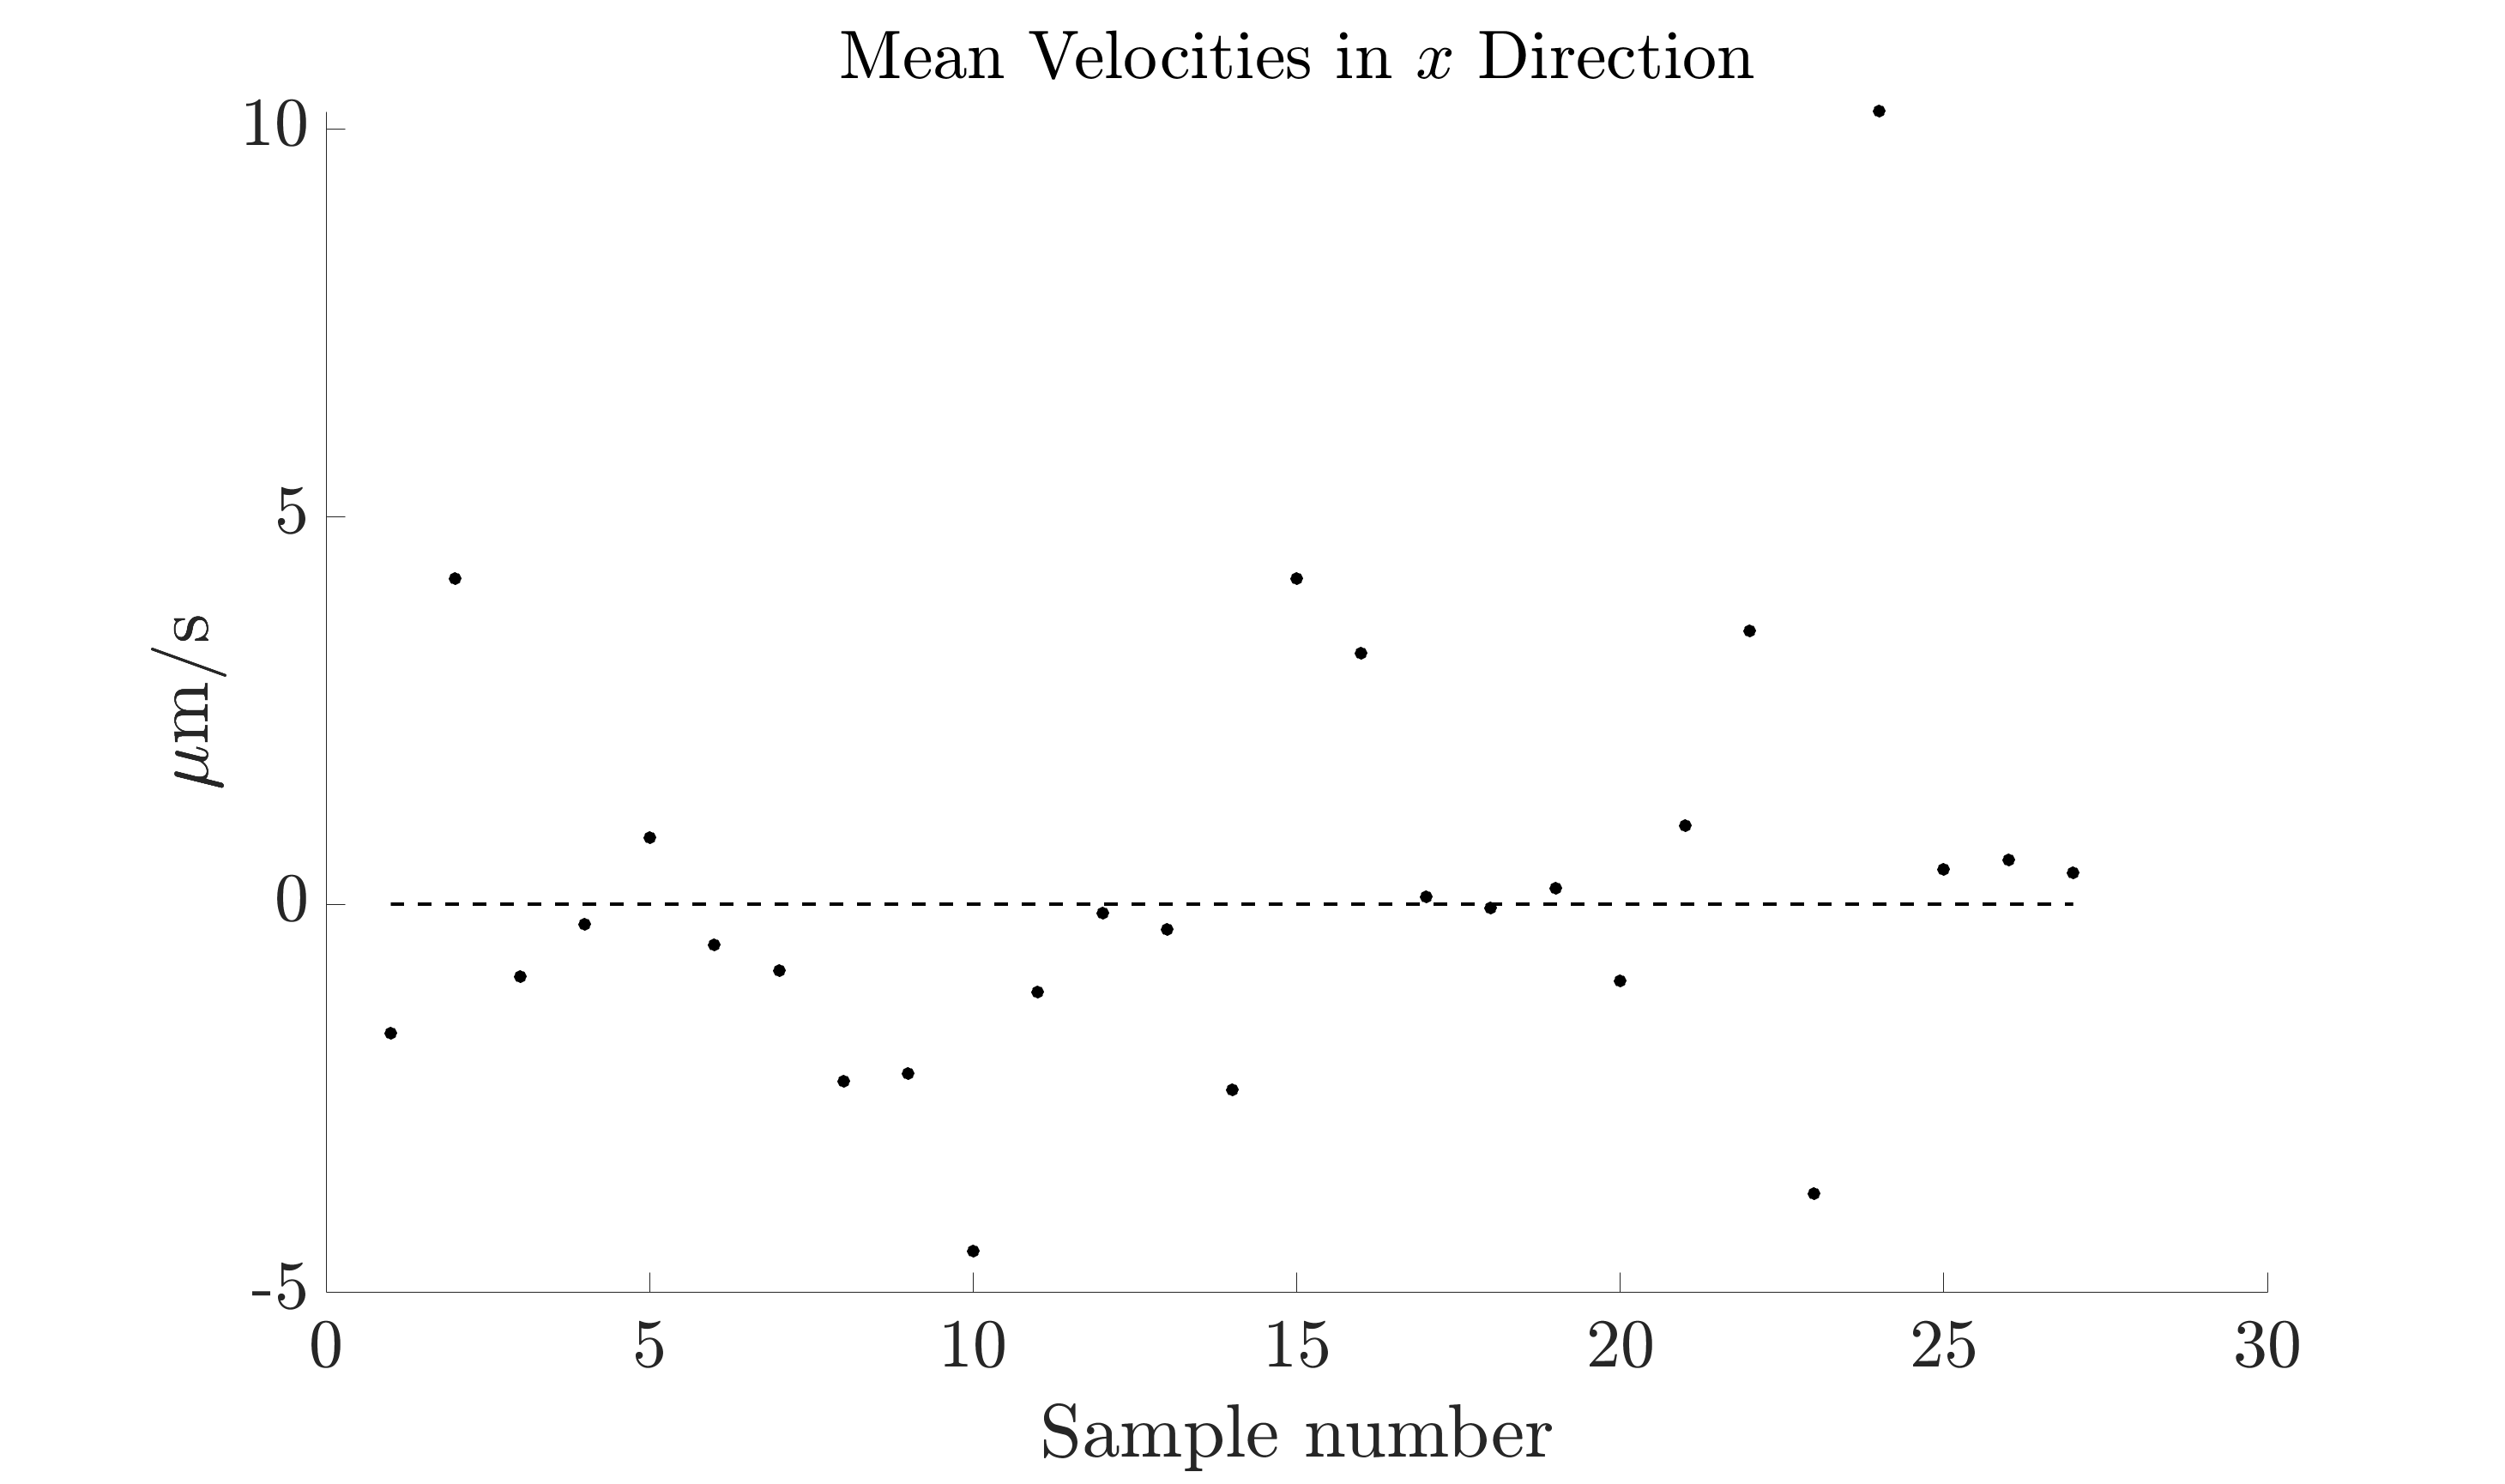
\includegraphics[width=\textwidth]{graphics/mean_velocities_x.png}
        \subcaption{Mean velocities in the $x$ direction of the particles tracked.}\label{fig:meanx}
    \end{minipage}
    \begin{minipage}[t]{0.49\textwidth}
        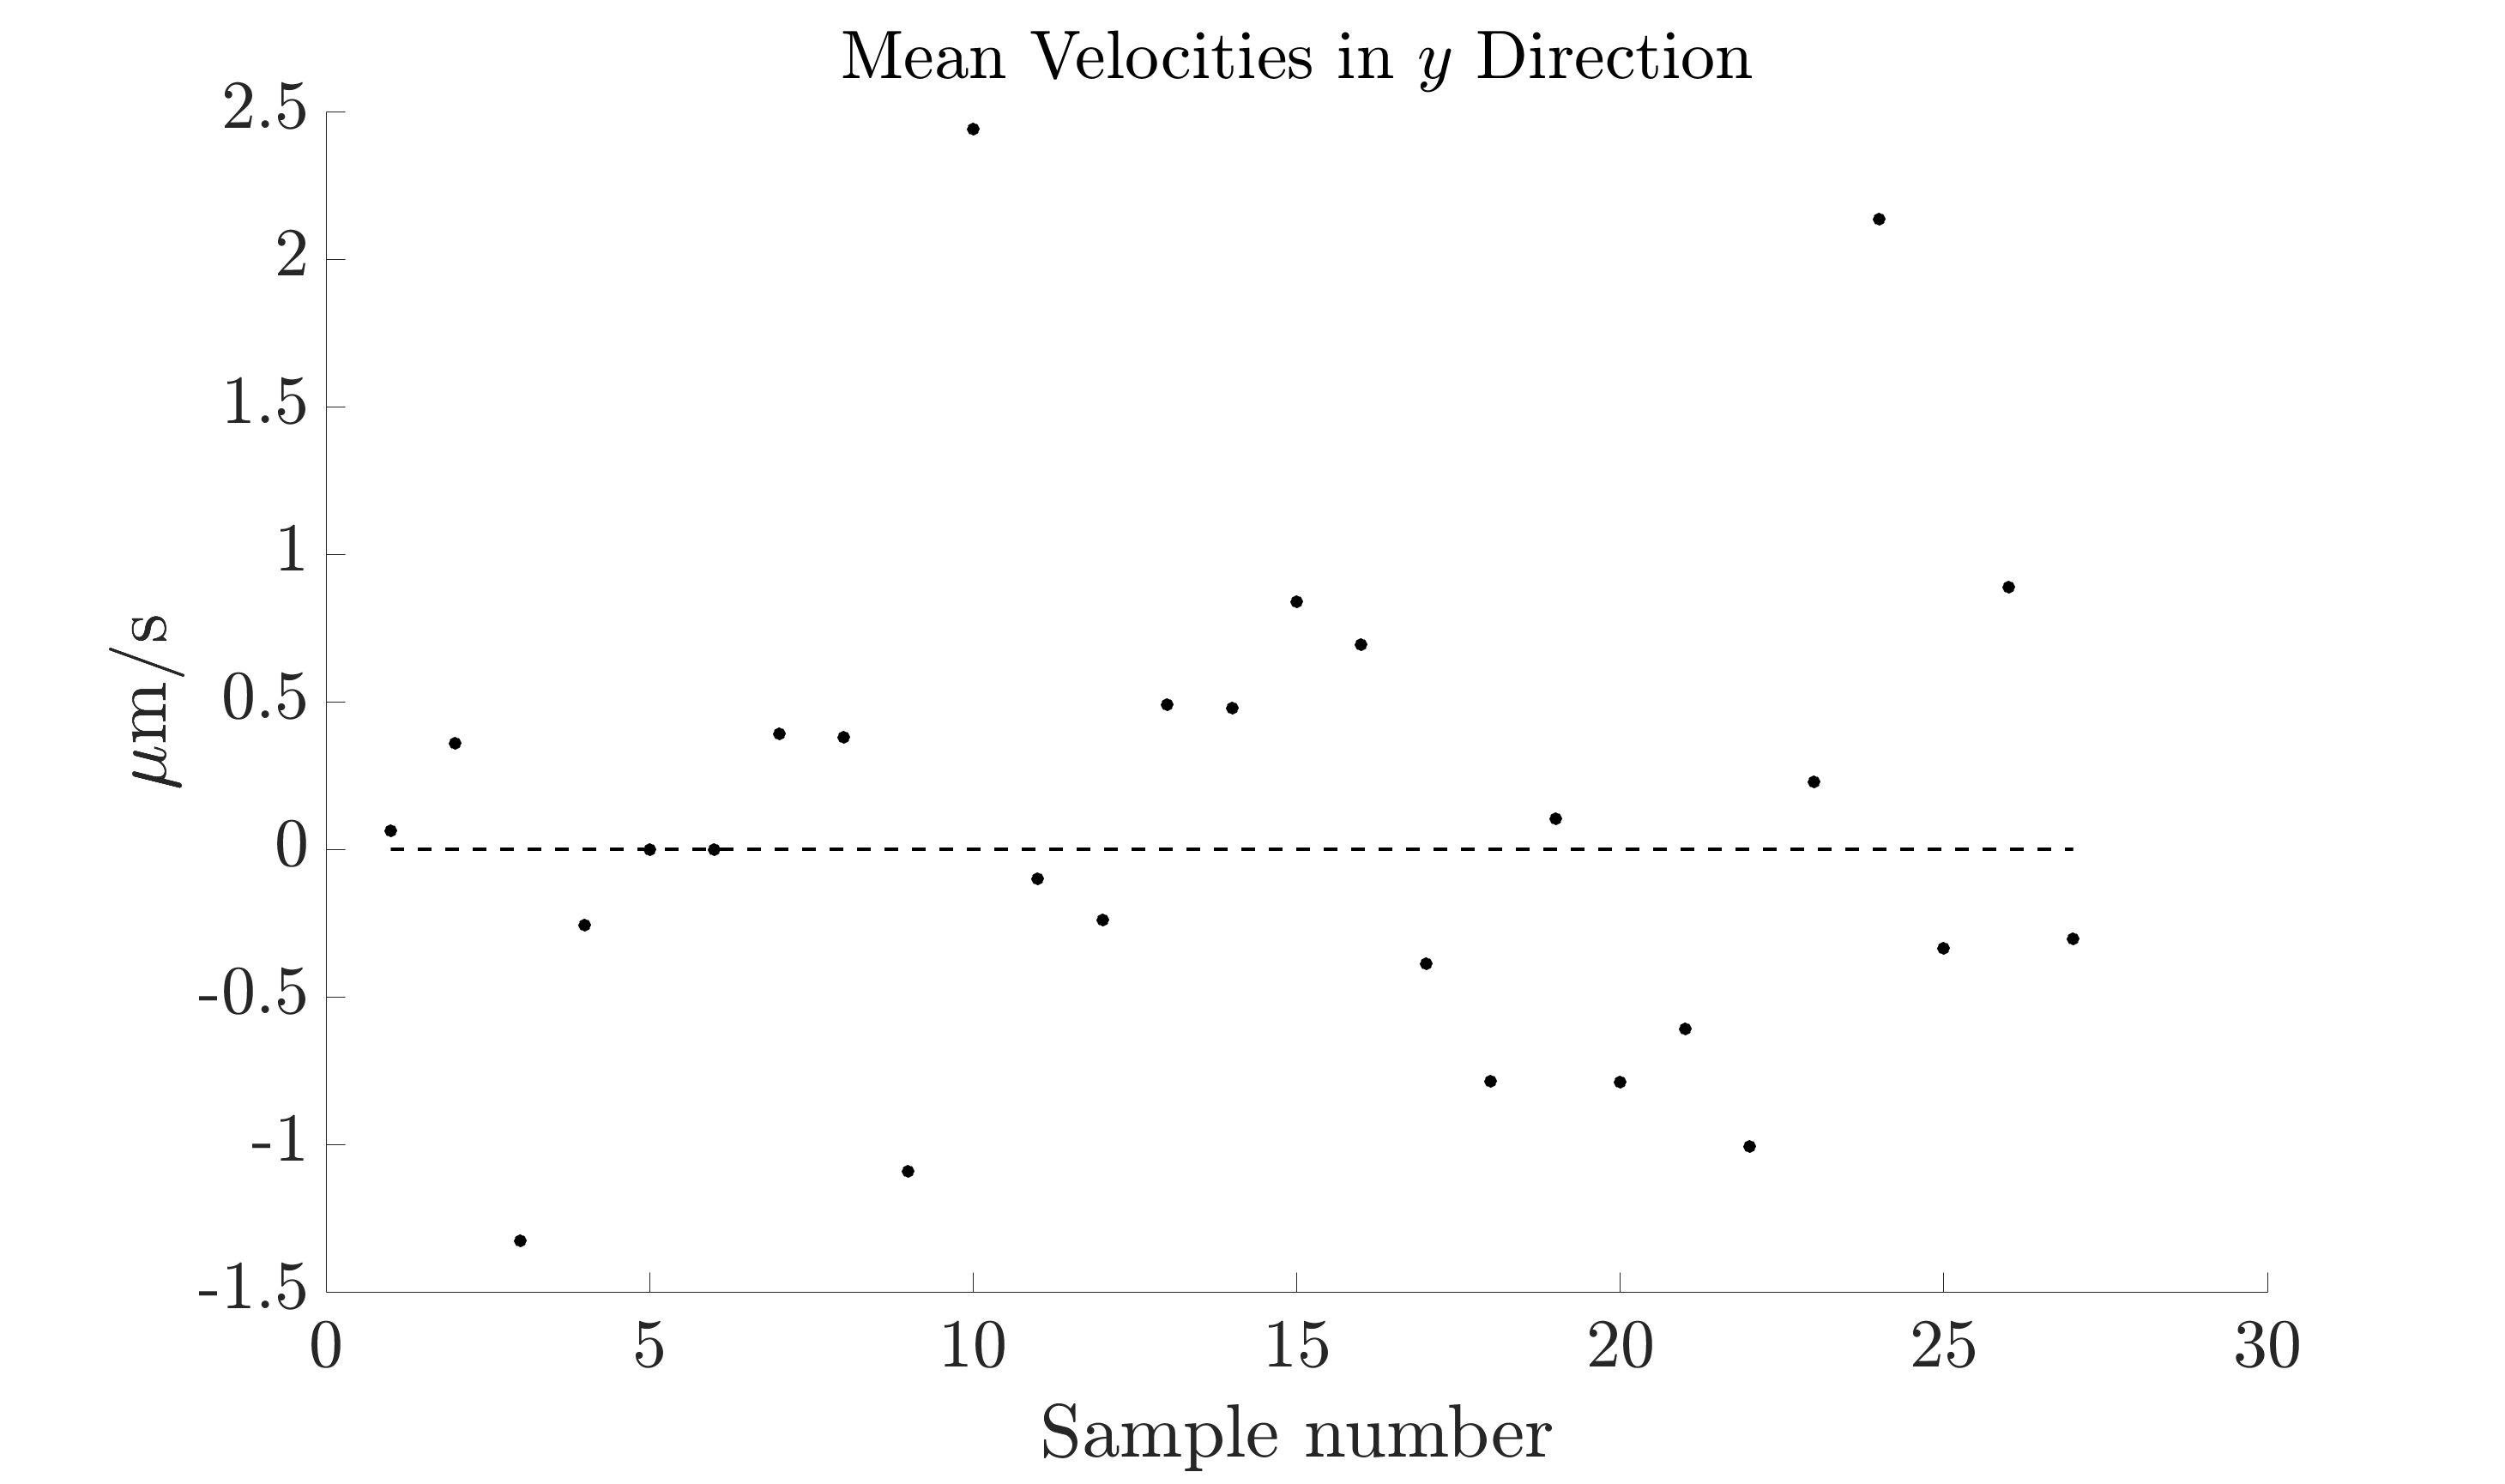
\includegraphics[width=\textwidth]{graphics/mean_velocities_y.png}
        \subcaption{Mean velocities in the $y$ direction of the particles tracked.}\label{fig:meany}
    \end{minipage} 
    \caption{Particle tracking data. The dashed horizontal line designates a value of zero.}\label{fig:particle_tracking_data}
\end{figure}
\clearpage
\bibliography{ref}{}
\end{document}
